% Формат А4, 12pt (ГОСТ Р 7.0.11-2011, 5.3.6)
\documentclass[a4paper,14pt]{extreport}

%%% Проверка используемого TeX-движка %%%
\usepackage{ifxetex}

%%% Поля и разметка страницы %%%
\usepackage{lscape}                                % Для включения альбомных страниц
\usepackage{geometry}                              % Для последующего задания полей
\usepackage{float}

%%% Математические пакеты %%%
\usepackage{amsthm,amsfonts,amsmath,amssymb,amscd} % Математические дополнения от AMS

%%% Кодировки и шрифты %%%
\ifxetex
  \usepackage{polyglossia}                         % Поддержка многоязычности
  \usepackage{fontspec}                            % TrueType-шрифты
\else
  \usepackage{cmap}                                % Улучшенный поиск русских слов в полученном pdf-файле
  \usepackage[T2A]{fontenc}                        % Поддержка русских букв
  \usepackage[utf8]{inputenc}                      % Кодировка utf8
  \usepackage[english, russian]{babel}             % Языки: русский, английский
  \usepackage{pscyr}                               % Красивые русские шрифты
\fi

%%% Оформление абзацев %%%
\usepackage{indentfirst}                           % Красная строка

%%% Цвета %%%
\usepackage[usenames]{color}
\usepackage{color}
\usepackage{colortbl}

%%% Таблицы %%%
\usepackage{longtable}                             % Длинные таблицы
\usepackage{multirow,makecell,array}               % Улучшенное форматирование таблиц

%%% Общее форматирование
\usepackage[singlelinecheck=off,center]{caption}   % Многострочные подписи
\usepackage{soul}                                  % Поддержка переносоустойчивых подчёркиваний и зачёркиваний
\usepackage{icomma}                                % Запятая в десятичных дробях

%%% Библиография %%%
\usepackage{cite}

%%% Гиперссылки %%%
\usepackage[plainpages=false,pdfpagelabels=false]{hyperref}

%%% Изображения %%%
\usepackage{graphicx}                              % Подключаем пакет работы с графикой

%%% Опционально %%%
% Следующий пакет может быть полезен, если надо ужать текст, чтобы сам текст не править, но чтобы места он занимал поменьше
%\usepackage{savetrees}

% Этот пакет может быть полезен для печати текста брошюрой
%\usepackage[print]{booklet}        % Подключаемые пакеты
%%% Макет страницы %%%
% Выставляем значения полей (ГОСТ 7.0.11-2011, 5.3.7)
\geometry{a4paper,top=2cm,bottom=2cm,left=2.5cm,right=1cm}

%%% Кодировки и шрифты %%%
\ifxetex
  \setmainlanguage{russian}
  \setotherlanguage{english}
  \defaultfontfeatures{Ligatures=TeX,Mapping=tex-text}
  \setmainfont{Times New Roman}
\else
  \renewcommand{\rmdefault}{ftm}    % Times New Roman
\fi

%%% Интервалы %%%
\linespread{1.3}                    % Полуторный интвервал (ГОСТ Р 7.0.11-2011, 5.3.6)

%%% Выравнивание и переносы %%%
\sloppy                             % Избавляемся от переполнений
\clubpenalty=10000                  % Запрещаем разрыв страницы после первой строки абзаца
\widowpenalty=10000                 % Запрещаем разрыв страницы после последней строки абзаца

%%% Библиография %%%
\makeatletter
\bibliographystyle{utf8gost71u}     % Оформляем библиографию по ГОСТ 7.1 (ГОСТ Р 7.0.11-2011, 5.6.7)
%\bibliographystyle{ugost2008}     % Оформляем библиографию по ГОСТ 7.1 (ГОСТ Р 7.0.11-2011, 5.6.7)
\renewcommand{\@biblabel}[1]{#1.}   % Заменяем библиографию с квадратных скобок на точку
\makeatother

%%% Изображения %%%
\graphicspath{{images/}}            % Пути к изображениям

%%% Цвета гиперссылок %%%
\definecolor{linkcolor}{rgb}{0.9,0,0}
\definecolor{citecolor}{rgb}{0,0.6,0}
\definecolor{urlcolor}{rgb}{0,0,1}
\hypersetup{
    colorlinks, linkcolor={linkcolor},
    citecolor={citecolor}, urlcolor={urlcolor}
}

%%% Оглавление %%%
\renewcommand{\cftchapdotsep}{\cftdotsep}

%%% Шаблон %%%
\newcommand{\todo}[1]{\textcolor{red}{#1}}

%%% Списки %%%
% Используем дефис для ненумерованных списков (ГОСТ 2.105-95, 4.1.7)
\renewcommand{\labelitemi}{\normalfont\bfseries{--}} 

%%% Колонтитулы %%%
% Порядковый номер страницы печатают на середине верхнего поля страницы (ГОСТ Р 7.0.11-2011, 5.3.8)
\makeatletter
\let\ps@plain\ps@fancy              % Подчиняем первые страницы каждой главы общим правилам
\makeatother
\pagestyle{fancy}                   % Меняем стиль оформления страниц
\fancyhf{}                          % Очищаем текущие значения
\fancyhead[C]{\thepage}             % Печатаем номер страницы на середине верхнего поля
\renewcommand{\headrulewidth}{0pt}  % Убираем разделительную линию
          % Пользовательские стили
%%% Основные сведения %%%
\newcommand{\thesisAuthor}             % Диссертация, ФИО автора
{Григорьев Семён Вячеславович}
\newcommand{\thesisTitle}              % Диссертация, название
{Cинтаксический анализ динамически формируемых строковых выражений}
\newcommand{\thesisSpecialtyNumber}    % Диссертация, специальность, номер
{05.13.11}
\newcommand{\thesisSpecialtyTitle}     % Диссертация, специальность, название
{Математическое и программное обеспечение вычислительных машин, комплексов и компьютерных сетей}
\newcommand{\thesisDegree}             % Диссертация, научная степень
{кандидата физико-математических наук}
\newcommand{\thesisCity}               % Диссертация, город защиты
{Санкт-Петербург}
\newcommand{\thesisYear}               % Диссертация, год защиты
{2015}
\newcommand{\thesisOrganization}       % Диссертация, организация
{кафедре системного программирования математико-механического факультета Санкт-Петербургского государственного университета}

\newcommand{\supervisorFio}            % Научный руководитель, ФИО
{Кознов Дмитрий Владимирович}
\newcommand{\supervisorRegalia}        % Научный руководитель, регалии
{кандидат физико-математических наук, доцент}

\newcommand{\opponentOneFio}           % Оппонент 1, ФИО
{Лисс Александр Рудольфович}
\newcommand{\opponentOneRegalia}       % Оппонент 1, регалии
{доктор технических наук, профессор, начальник исследовательского отделения}
\newcommand{\opponentOneJobPlace}      % Оппонент 1, место работы
{ОАО ``Концерн ``ОкеанПрибор''}
\newcommand{\opponentOneJobPost}       % Оппонент 1, должность
{}

\newcommand{\opponentTwoFio}           % Оппонент 2, ФИО
{Ицыксон Владимир Михайлович}
\newcommand{\opponentTwoRegalia}       % Оппонент 2, регалии
{кандидат технических наук, доцент}
\newcommand{\opponentTwoJobPlace}      % Оппонент 2, место работы
{ФГБОУ ВПО ``Санкт-Петербургский государственный политехнический университет''}
\newcommand{\opponentTwoJobPost}       % Оппонент 2, должность
{\todo{ }}

\newcommand{\leadingOrganizationLines} % Ведущая организация, дополнительные строки
{\\~\\~\\~}
\newcommand{\leadingOrganizationTitle} % Ведущая организация, дополнительные строки
{\todo{ }}

\newcommand{\defenseDate}              % Защита, дата
{\todo{}}% г.~в~  часов}}
\newcommand{\defenseCouncilNumber}     % Защита, номер диссертационного совета
{Д 212.232.51}
\newcommand{\defenseCouncilTitle}      % Защита, учреждение диссертационного совета
{Санкт-Петербургского государcтвенного университета}
\newcommand{\defenseCouncilAddress}    % Защита, адрес учреждение диссертационного совета
{198504, Санкт-Петербург, Петродворец, Университетский пр., 28, математико-механический факультет, ауд. 405}

\newcommand{\defenseSecretaryFio}      % Секретарь диссертационного совета, ФИО
{Косовский Николай Кириллович}
\newcommand{\defenseSecretaryRegalia}  % Секретарь диссертационного совета, регалии
{д.ф.-м.н., профессор}

\newcommand{\synopsisLibrary}          % Автореферат, название библиотеки
{Научной библиотеке Санкт-Петербургского государственного университета по адресу: 199034, Санкт-Петербург, Университетская наб., д. 7/9}
\newcommand{\synopsisDate}             % Автореферат, дата рассылки
{\todo{  }}%года}}
            % Основные сведения

\newtheoremstyle{mystyle}%                % Name
  {}%                                     % Space above
  {}%                                     % Space below
  {\itshape}%                             % Body font
  {}%                                     % Indent amount
  {\scshape}%                            % Theorem head font
  {.}%                                    % Punctuation after theorem head
  { }%                                    % Space after theorem head, ' ', or \newline
  {}%                                     % Theorem head spec (can be left empty, meaning `normal')

\theoremstyle{mystyle}

\begin{document}

\algtext*{EndWhile}% Remove "end while" text
\algtext*{EndIf}% Remove "end if" text
\algtext*{EndFor}% Remove "end for" text
\algtext*{EndFunction}% Remove "end function" text
%\declaretheoremstyle[headfont=\normalfont]{normalhead}
%\declaretheorem[style=normalhead]{example}
%\theoremheaderfont{\textsc}
\newtheorem{mydef}{Определение}
\renewcommand{\lstlistingname}{Листинг}
\renewcommand\listingscaption{Листинг}


%%% Переопределение именований %%%
\renewcommand{\abstractname}{Аннотация}
\renewcommand{\alsoname}{см. также}
\renewcommand{\appendixname}{Приложение}
\renewcommand{\bibname}{Литература}
\renewcommand{\ccname}{исх.}
\renewcommand{\chaptername}{Глава}
\renewcommand{\contentsname}{Содержание}
\renewcommand{\enclname}{вкл.}
\renewcommand{\figurename}{Рисунок} % (ГОСТ Р 7.0.11-2011, 5.3.9)
\renewcommand{\headtoname}{вх.}
\renewcommand{\indexname}{Предметный указатель}
\renewcommand{\listfigurename}{Список рисунков}
\renewcommand{\listtablename}{Список таблиц}
\renewcommand{\pagename}{Стр.}
\renewcommand{\partname}{Часть}
\renewcommand{\refname}{Список литературы}
\renewcommand{\seename}{см.}
\renewcommand{\tablename}{Таблица} % (ГОСТ Р 7.0.11-2011, 5.3.10)           % Переопределение именований

% Структура диссертации (ГОСТ Р 7.0.11-2011, 4)
\newcommand{\sfs}{\fontsize{14pt}{15pt}\selectfont}
\sfs % размер шрифта и расстояния между строками
\thispagestyle{empty}

\vspace{10mm}
\begin{flushright}
  \Large{На правах рукописи}
  %
\includegraphics[height=1.5cm]{personal-signature} 
\end{flushright}

\vspace{30mm}
\begin{center}
{\Large\bf{\thesisAuthor}}
\end{center}

\vspace{30mm}
\begin{center}
{\bf \LARGE \thesisTitle \par}

\vspace{30mm}
{\Large Специальность \thesisSpecialtyNumber~---\par \thesisSpecialtyTitle}

\vspace{15mm}
\LARGE{Автореферат}\par
\Large{диссертации на соискание учёной степени\par \thesisDegree}
\end{center}

%\vspace{15mm}
%\begin{tabular}{p{6cm} r p{3cm}}
%&Председатель:& \\
%%& & \\
%Оппонент:&     \\                     
%%& & \\
%&Научный руководитель:& \\
%%& & \\
%&Соискатель:&  \\
%\end{tabular}

\vspace{20mm}
\begin{center}
{\Large{\thesisCity~--- \thesisYear}}
\end{center}

\newpage
% оборотная сторона обложки
\thispagestyle{empty}
\noindent Работа выполнена на \thesisOrganization

\begin{table} [h]  
  \begin{tabular}{ll}  
   \makecell[l]{\sfs Научный руководитель:\\~} &
   \makecell*[{{p{11cm}}}]{\sfs
   \supervisorRegalia \\ \textbf{\sfs \supervisorFio}}
      
\vspace{3mm} \\

   \makecell[l]{\sfs Официальные оппоненты:} &
   \makecell*[{{p{11cm}}}]{\sfs \textbf{\opponentOneFio,}} \\
   &
   \makecell[{{p{11cm}}}]{
    \sfs \opponentOneRegalia \\
    \sfs \opponentOneJobPlace,  
    \sfs \opponentOneJobPost 
    \vspace{3mm} \\
    \sfs \textbf{\opponentTwoFio,} \vspace{1mm}\\
    \sfs \opponentTwoRegalia \\
    \sfs \opponentTwoJobPlace, 
    \sfs \opponentTwoJobPost
   }

\vspace{3mm} \\

   \makecell[l]{\sfs Ведущая организация: \leadingOrganizationLines} &
   \makecell*[{{p{11cm}}}]{\sfs
   \leadingOrganizationTitle
   }
  \end{tabular}  
\end{table}

\noindent Защита состоится \defenseDate~на~заседании диссертационного совета \defenseCouncilNumber~на базе \defenseCouncilTitle~по адресу: \defenseCouncilAddress.

\vspace{5mm}
\noindent С диссертацией можно ознакомиться в \synopsisLibrary.

\vspace{5mm}
\noindent{Автореферат разослан \synopsisDate}%.}

\vspace{5mm}
\begin{table} [h]
  \begin{tabular}{p{8cm}cr}
    \begin{tabular}{p{8cm}}
      \sfs Ученый секретарь  \\
      \sfs диссертационного совета  \\
      \sfs \defenseCouncilNumber, \defenseSecretaryRegalia
    \end{tabular} 
    & \begin{tabular}{c}
       %
\includegraphics[height=1cm]{secretary-signature} 
    \end{tabular} 
    & \begin{tabular}{r}
       \\
       \\
       \sfs \defenseSecretaryFio
    \end{tabular} 
  \end{tabular}
\end{table}
\newpage
           % Титульный лист
% Оглавление (ГОСТ Р 7.0.11-2011, 5.2)
\ifdefmacro{\microtypesetup}{\microtypesetup{protrusion=false}}{} % не рекомендуется применять пакет микротипографики к автоматически генерируемому оглавлению
\tableofcontents*
\addtocontents{toc}{\protect\tocheader}
\endTOCtrue
\ifdefmacro{\microtypesetup}{\microtypesetup{protrusion=true}}{}        % Оглавление
\chapter*{Введение}                         % Заголовок
\addcontentsline{toc}{chapter}{Введение}    % Добавляем его в оглавление
\textbf{Актуальность работы}

Статический анализ исходного кода является известной техникой  получения знаний о программе без её исполнения ~\cite{StaticCodeAnalysis3,StaticCodeAnalysis2,StaticCodeAnalysis1}. Статический анализ является неотъемлемой частью многих процессов, связанных с разработкой программного обеспечения (ПО), и может использоваться, например, для упрощения работы с кодом с помощью подсветки синтаксиса языка в программах, навигации по коду, реализации контекстных подсказок. Более того, статический анализ используется для обнаружения ошибок на ранних стадиях разработки, до запуска программы, а также для поиска различных семантических ошибок, которые не могут быть определены обычным синтаксическим анализом.  Также, статический анализ используется при решении задач трансформации исходного кода и реинжиниринге~\cite{reengANT}. Однако во многих языках программирования имеются конструкции, которые существенно затрудняют статический анализ. 

Например, широко используются динамические встроенные языки --- приложение, созданное на одном языке, генерирует программу на другом языке и передаёт её на выполнение в соответствующее окружение. Примерами могут служить динамические SQL-запросы к базам данных из приложений на Java, С++, С\#, формирование HTML-страниц в PHP-приложениях~\cite{DSQLISO,JSP,PHPmySQL}. Генерируемый код собирается из строк таким образом, чтобы в момент выполнения результирующая строка представляла собой корректную программу. Примеры использования встроенных языков представлены в листингах~\ref{lst:dsql1},~\ref{lst:JsJava} и~\ref{lst:PhPSqlHtml}. Следует отметить, что одна программа может генерировать код на нескольких языках (см. листинг~\ref{lst:PhPSqlHtml}). При этом возможно получение частей кода из разных источников (например, учитывать текстовый ввод пользователя, что часто используется для задания фильтров при конструировании SQL-запросов). Использование динамически формируемых программ  позволяет избежать дополнительных накладных расходов, присущих таким технологиям, как ORM\footnote{ORM или Object-Relational Mapping --- технология программирования, которая связывает базы данных с концепциями объектно-ориентированных языков программирования~\cite{ORM}.}, и достичь высокой производительности. Благодаря этому использование динамически генерируемых программ получило широкое распространение и применяется до сих пор. Вместе с этим, несмотря на появление новых технологий, динамическая генерация SQL-запросов активно используется и в настоящее время~\cite{DSQLInActiveUse}.

\fvset{frame=lines,framesep=5pt,fontsize=\small}\

\begin{listing}
    \begin{pyglist}[language=sql,numbers=left,numbersep=5pt]

CREATE PROCEDURE [dbo].[MyProc]  @TABLERes   VarChar(30)
AS
    EXECUTE ('INSERT INTO ' + @TABLERes + ' (sText1)' +
             ' SELECT ''Additional condition: '' + sName' +
             ' from #tt where sAction = ''1000000''')
GO
    \end{pyglist}
\caption{Код с использованием динамического SQL}
\label{lst:dsql1}
\end{listing} 
 
\fvset{frame=lines,framesep=5pt}
\begin{listing}
    \begin{pyglist}[language=java,numbers=left,numbersep=5pt]
import javax.script.*;  
public class InvokeScriptFunction {  
    public static void main(String[] args) throws Exception {  
        ScriptEngineManager manager = new ScriptEngineManager();  
        ScriptEngine engine = manager.getEngineByName("JavaScript");  
        // JavaScript code in a String  
        String script = 
            "function hello(name) { print('Hello, ' + name); }";  
        // evaluate script  
        engine.eval(script);  
        // javax.script.Invocable is an optional interface.  
        // Check whether your script engine implements or not!  
        // Note that the JavaScript engine implements
        // Invocable interface.  
        Invocable inv = (Invocable) engine;  
        // invoke the global function named "hello"  
        inv.invokeFunction("hello", "Scripting!!" );  
    }  
}
    \end{pyglist}
\caption{Вызов JavaScript из Java}
\label{lst:JsJava}
\end{listing}


\fvset{frame=lines,framesep=5pt}
\begin{listing}
    \begin{pyglist}[language=php,numbers=left,numbersep=5pt]

<?php
    // Embedded SQL
    $query = 'SELECT * FROM ' . $my_table; 
    $result = mysql_query($query);
    
    // HTML markup generation
    echo "<table>\n";
    while ($line = mysql_fetch_array($result, MYSQL_ASSOC)) {
        echo "\t<tr>\n";    
        foreach ($line as $col_value) {
            echo "\t\t<td>$col_value</td>\n";
        }
        echo "\t</tr>\n";
    }
    echo "</table>\n";
?>
    \end{pyglist}
\caption{Использование нескольких встроенных в PHP языков (MySQL, HTML)}
\label{lst:PhPSqlHtml}
\end{listing}



Динамически формируемые выражения часто конструируются с помощью таких операций, как конкатенация в циклах или условных предложениях, или в рекурсивных процедурах. Это затрудняет статический анализ и приводит к получению множества возможных значений для каждого выражения в момент выполнения. Вследствие этого фрагменты динамически формируемого кода воспринимаются компилятором исходного языка как простые строки, не подлежащие дополнительному анализу, а это, в свою очередь, приводит к высокой вероятности возникновения ошибок во время выполнения программы. В худшем случае такая ошибка не приведёт к прекращению работы приложения, что указало бы на проблемы, однако целостность данных при этом может оказаться нарушена. Более того, использование динамически формируемых выражений затрудняет не только разработку информационных систем, так и также и реинжиниринг, поскольку в последнем случае важно автоматизировать перенос системы на новые зыки и платформы, что невозможно без качественного статического анализа. Например, при наличии в коде приложения динамически формируемых SQL-запросов нельзя точно ответить на вопрос о том, с какими элементами базы данных не взаимодействует система, и удалить их. При переносе такой системы на другую СУБД необходимо гарантировать, что для всех динамически формируемых выражений значение в момент выполнения будет корректным кодом на языке новой СУБД~\cite{JSquash}. Следует отметить, что отсутствие статического анализа динамически формируемых программ не позволяет реализовывать для них стандартную функциональность интегрированных сред разработки (Integrated Development Environment, IDE) --- подсветку синтаксиса и автодополнение, рефакторинг кода и т.д. Такая функциональность значительно упрощает процесс разработки и отладки приложений и полезна не только для основного языка, но и для встроенных языков. 

Для решения всех перечисленных выше задач необходимы инструменты, проводящие статический анализ динамически формируемых программ. Такой анализ может дать существенную информацию о таких программах, поскольку редко встречается ситуация полной динамической неопределённости (например, при создании динамических программ исключительно на основе пользовательского ввода). В большинстве случаев, имея программу, генерирующую динамические вставки, с помощью статического анализа можно получить достаточно информации для решения поставленных выше задач. Решению этой проблемы и посвящена данная диссертационная работа. 


\textbf{Степень разработанности темы}

Существуют классические исследования, посвященные разработке компиляторов --- работы А.~Ахо~\cite{Dragon}, А.~Брукера~\cite{CompilerCompiler}, С.~Джонсона~\cite{yaccBook},  Б.К.Мартыненко~\cite{Martinenko1, Martinenko2}  и др.  Однако содержащиеся там алгоритмы синтаксического анализа не могут быть применены к решению задачи анализа динамически формируемых программ, поскольку предназначены для обработки входных данных, представимых в видн линейной последовательности символов, а такое представление динамически формируемых программ не всегда возможно.

Методы обобщённого синтаксического анализа, лежащие в основе данной работы, изложены в трудах таких учёных как Масару Томита (Masaru Tomita)~\cite{Tomita}, Элизабет Скотт (Elizabeth Scott) и Адриан Джонстон (Adrian Johnstone)~\cite{RNGLR,RIGLR} из университета Royal Holloway (Великобритания), Ян Рекерс (Jan Rekers, University of Amsterdam)~\cite{SPPF}, Элко Виссер (Eelco Visser)~\cite{RNGLRSyntaxerror2,RNGLRSyntaxerror3} и других.

Анализу динамически формируемых строковых выражений посвящены работы таких зарубежных учёных как Кюнг-Гу Дох (Kyung-Goo Doh)~\cite{LrAbstract1,LrAbstract2,LRAbstractParsingSema}, Ясухико Минамиде (Minamide Yasuhiko)~\cite{PHPSA}, Андерс Мёллер (Anders M{\o}ller)~\cite{JSA} и отечественных учёных А.А.~Бреслава~\cite{Alvor1,Alvor2} и других. Хорошо изучены вопросы проверки корректности динамически формируемых выражений и поиска фрагментов кода, уязвимых для SQL-инъекций~\cite{SQLInjection,Dasgupta:2009:SAF:1546683.1547548}. Однако данные работы исследуют отдельные аспекты проблемы статического анализа динамически формируемых программ, оставляя в стороне создание готовых алгоритмов (в частности, не строят структурное представление анализируемых программ). В связи с этим возникают проблемы масштабируемости данных результатов, например, создание на их основе более сложных видов статического анализа.

Так же важным является предоставление компонентов, упрощающих создание новых инструментов для решения конкретных задач. Данных подход хорошо исследован в области разработки компиляторов, где широкое распространение получили генераторы анализаторов и пакеты стандартных библиотек (работы А.~Ахо~\cite{Dragon}, А.~Брукера~\cite{CompilerCompiler}, С.~Джонсона~\cite{yaccBook} и др.). 

В работах отечественных учёных М.Д.~Шапот и Э.В.~Попова~\cite{DynamicDSQLTranslation}, а так же зарубежных учёных Антони Клеви (Anthony Cleve), Жан-Люк Эно (Jean-Luc Hainaut)~\cite{DSQLReverseEngineering}, Йост Виссер (Joost Visser)~\cite{DSQLQualityMesure} и других рассматриваются различные аспекты реинжиниринга информационных систем, использующих встроенные SQL-запросы, однако не формулируется общего метода для решения таких задач. Этот вопрос также не затрагивается в классических работах, посвященных реинжиниригу~\cite{SoftwareReeng1, reengANT, SoftwareReeng2, SoftwareReeng3}. Однако разработка такого метода является актуальной задачей.

Таким образом, актуальной является задача дальнейшего исследования статического анализа динамически формируемых строковых выражений. Кроме этого важным является решение вопросов практического применения средств анализа динамически формируемого кода: упрощение разработки инструментов анализа и создание методов их применения в реинжиниринге программного обеспечения.
\textbf{Объект исследования}

Объектом исследования являются методы, алгоритмы и программные средства обработки динамически формируемых программ, а также задача реинжиниринга информационных систем.

\textbf{Цель и задачи диссертационной работы}

\textbf{Целью} данной работы является создание комплексного подхода к статическому синтаксическому анализу динамически формируемых программ.

Достижение поставленной цели обеспечивается решением следующих \textbf{задач}.
\begin{enumerate}
    \item Разработать универсальный алгоритм синтаксического анализа динамически формируемых программ, не зависящий от целевого языка программирования и допускающий реализацию различных видов статического анализа. 
    \item Создать архитектуру инструментария для автоматизации разработки программных средств статического анализа динамически формируемых программ.
    \item Создать метод реинжиниринга динамически формируемых программ.
\end{enumerate}

\textbf{Методология и методы исследования}

Методология исследования основана на подходе к спецификации и анализу формальных языков, активно развивающемуся с 50-х годов 20-го века (см., например, работы Н. Хомского~\cite{chomskyMethod ,chomskySyntactic}). В последствии этот подход получил широкое распространение в областях, связанных с обработкой языков программирования.
Основными элементами данного подхода являются алфавит и грамматика языка, разбиение автоматической обработки языка на выполнение таких шагов как лексический, синтаксический и семантический анализ. Решаемые в связи с этим задачи связаны с поиском эффективных алгоритмов, выполняющих эти шаги. 

В работе применяется алгоритм обобщённого восходящего синтаксического анализа RNGLR~\cite{RNGLR}, созданный Элизабет Скотт (Elizabeth Scott) и Адриан Джонстон (Adrian Johnstone) из университета Royal Holloway (Великобритания). Для компактного хранения леса вывода использовалась структура данных Shared Packed Parse Forest (SPPF), которую предложил Ян Рекерс (Jan Rekers, University of Amsterdam)~\cite{SPPF}.

Доказательство завершаемости и корректности предложенного алгоритма проводилось с применением теории формальных языков, теории графов и теории сложности алгоритмов. Приближение множества значений динамически формируемого выражения строилось в виде регулярного множества, описываемого с помощью конечного автомата.


\textbf{Положения, выносимые на защиту}
\begin{enumerate}
    \item Разработан алгоритм синтаксического анализа динамически формируемых программ, позволяющий обрабатывать произвольную регулярную аппроксимацию множества значений выражения в точке выполнения, реализующий эффективное управление стеком и гарантирующий конечность представления леса вывода. Доказана завершаемость и корректность предложенного алгоритма при обработке регулярной аппроксимации, представимой в виде произвольного конечного автомата без $\varepsilon$-переходов. 
    \item Создана архитектура инструментария для разработки программных средств статического анализа динамически формируемых программ.
    \item Разработан метод анализа и обработки динамически формируемых программ в проектах по реинжинирингу информационных систем. 
\end{enumerate}

\textbf{Научная новизна работы}

Научная новизна полученных в ходе исследования результатов заключается в следующем.

\begin{enumerate}

\item Алгоритм, предложенный в диссертации, отличается от аналогов (работы Андрея Бреслава~\cite{Alvor1, Alvor2}, Кюнг-Гу Дох~\cite{LrAbstract1, LrAbstract2}, Ясухико Минамиде~\cite{PHPSA}) возможностью построения компактной структуры данных, содержащей деревья вывода для всех корректных значений выражения. Это позволяет использовать результаты работы алгоритма для проведения более сложных видов анализа. Алгоритмы, представленные в (JSA~\cite{JSA}~\cite{Alvor1, Alvor2}, PHPSA~\cite{PHPSA}) предназначены только для проверки корректности выражений, основанной на решении задачи о включении одного языка в другой. Выполнение более сложных видов анализа, трансформаций или построения леса разбора не предполагается. 

\item Новизна представленной архитектуры заключается в том, что она позволяет создать платформу для разработки целевых инструментов, решающих широкий круг задач анализа динамически формируемого кода. Существующие архитектуры готовых инструментов (JSA, PHPSA, Alvor, Varis) предназначены для решения конкретных задач для определённых языков. Решение новых задач или поддержка других языков с помощью этих инструментов затруднены ввиду ограничений, накладываемых архитектурой и возможностями используемого алгоритма анализа. 

\item Метод анализа и обработки встроенного программного кода в проектах по реинжинирингу информационных систем предложен впервые. К.В.~Ахтырченко и Т.П.~Сорокваша отмечают~\cite{SoftwareReengMethods}, что существующие работы в области реинжиниринга программного обеспечения либо содержат высокоуровневые решения, не касающиеся деталей, важных при решении прикладных задач (например, работы К. Вагнера~\cite{SoftwareReeng3}, Х. Миллера~\cite{SoftwareReeng2}), либо являются набором подходов к решению конкретных задач (например, работы~\cite{SoftwareReeng1, reengANT, boulychev}). При этом, встроенный программный код часто не учитывается. С другой стороны, работы М.Д.~Шапот и Э.В.~Попова~\cite{DynamicDSQLTranslation}, С.Л.~Трошина~\cite{reengANT}, А.~Клеви~\cite{DSQLReverseEngineering}  посвящены решению конкретных задач обработки встроенного программного кода в контексте реинжиниринга информационных систем, но не предлагают обобщённого и масштабируемого метода.

\end{enumerate}


\textbf{Теоретическая и практическая значимость работы}

Теоретическая значимость диссертационного исследования заключается в разработке формального алгоритма синтаксического анализа динамически формируемого кода, решающего задачу построения конечного представления леса вывода, не решенную полностью ранее, а также в формальном доказательстве завершаемости и корректности разработанного алгоритма. 

На основе полученных в работе научных результатов был разработан инструментарий (Software Development Kit, SDK), предназначенный для создания средств статического анализа динамически формируемых программ. 
С использованием разработанного инструментария было реализовано расширение к инструменту ReSharper (ООО ``ИнтеллиДжей Лабс'', Россия), предоставляющее поддержку встроенного T-SQL в проектах на языке программирования C\# в среде разработки Microsoft Visual Studio. Так же было выполнено внедрение результатов работы в промышленный проект по переносу хранимого SQL-кода с MS-SQL Server 2005 на Oraclе 11gR2 (ЗАО ``Ланит-Терком'', Россия). 

\textbf{Степень достоверности и апробация результатов}

Достоверность и обоснованность результатов исследования опирается на использование формальных методов исследуемой области, проведенные доказательства, рассуждения и эксперименты.

Основные результаты работы были доложены на ряде научных конференций: SECR-2012, SECR-2013, SECR-2014, TMPA-2014, Parsing@SLE-2013, Рабочий семинар ``Наукоемкое программное обеспечение'' при конференции PSI-2014. Доклад на SECR-2014 награждён премией Бертрана Мейера за лучшую исследовательскую работу в области программной инженерии. Дополнительной апробацией является то, что разработка инструментальных средств на основе предложенного алгоритма была поддержана Фондом содействия развитию малых форм предприятий в технической сфере (программа УМНИК~\cite{UMNIC}, проекты \textnumero~162ГУ1/2013 и \textnumero~5609ГУ1/2014).

\textbf{Публикации по теме диссертации}

Все результаты диссертации изложены в 7 научных работах, из которых 3~\cite{YCArticle,SELforIDEru,AbstractGLL}, содержащие основные результаты, опубликованы в журналах из ‘’Перечня российских рецензируемых научных журналов, в которых должны быть опубликованы основные научные результаты диссертаций на соискание ученых степеней доктора и кандидата наук’’, рекомендовано ВАК. 
1 работа~\cite{GLRAbsPars} индексируются Scopus. В работах, написанных в соавторстве, вклад автора определяется следующим образом.  В~\cite{Syrcose} С. Григорьеву принадлежит реализация ядра платформы YaccConstructor. В~\cite{SELforIDEru, AbstractGLL} и~\cite{SELforIDE} С. Григорьеву принадлежит постановка задачи, формулирование требований к разрабатываемым инструментальным средствам, работа над текстом. 
В~\cite{GLRAbsPars} автору принадлежит идея, описание и реализация анализа встроенных языков на основе RNGLR алгоритма.  В~\cite{YCArticle} С. Григорьеву принадлежит реализация инструментальных средств, проведение экспериментов, работа над текстом. В работе~\cite{RelaxedARNGLR} автору принадлежит алгоритм синтаксического анализа динамически формируемого кода.


\textbf{Структура работы}

Диссертация состоит из введения, шести глав, заключения и построена следующим образом. В первой главе приводится обзор области исследования. Рассматриваются подходы к анализу динамически формируемых строковых выражений и соответствующие инструменты. Описывается алгоритм обобщённого восходящего синтаксического анализа RNGLR, взятый за основу в диссертационной работе. Также описываются проекты YaccConstructor и ReSharper SDK, использованные для реализации предложенного в работе инструментария. Во второй главе формализуется основная задача исследования и излагается решающий её алгоритм синтаксического анализа регулярных множеств. Приводится доказательство завершаемости и корректности представленного алгоритма, приводятся примеры. В третьей главе описывается инструментальный пакет YC.SEL.SDK, разработанного на основе алгоритма, описанного во второй главе и предназначеного для разработки инструментов анализа динамически формируемых программ. Описывается архитектура компонентов и особенности их реализации. Также описывается YC.SEL.SDK.ReSharper --- ``обёртка'' для YC.SEL.SDK, позволяющая создавать расширения к ReSharper для поддержки встроенных языков. В четвёртой главе описывается метод реинжиниринга встроенного программного кода.  В пятой главе приводятся результаты экспериментального исследования разработанного алгоритма и инструмента YC.SEL.SDK. Шестая глава содержит результаты сравнения и соотнесения полученных результатов с  существующими аналогами.

\textbf{Благодарности}

А.Н.Терехову, работкникам и администрации компании ЗАО ``Ланит-Терком'' за создания условий для изучения данной темы (организация проектов по реинжинирингу). Я.А.Кириленко за погружение в тему исследования и руководство на начальных этапах. Д.Ю.Булычеву за помощь в уточнении постановки задачи исследования и в написании статей. Студентам и аспирантам кафедры системного программирования Дмитрию Авдюхину, Анастасии Рагозиной, Екатерине Вербицкой, Марине Полубеловой, Иванову Андрею за помощь в реализации предложенных идей и проведение экспериментов. Отдельную благодарность  хочется выразить компании ООО ``ИнтеллиДжей Лабс'' и Андрею Иванову за поддержку исследований. Также хочется поблагодарить А.К.Петренко и В.М.Ицыксона, а также сотрудников ИСП РАН за ценные вопросы и комментарии к работе, позволившие уточнить ряд формулировок и улучшить изложение результатов. 
    % Введение
\chapter{Обзор} \label{relWorks}

В данной главе введены основные термины и определения, используемые в работе, а также рассмотрены основные подходы к анализу встроенных языков и инструменты для их обработки. Также рассмотрен алгоритм обобщённого восходящего синтаксического анализа RNGLR, лежащий в основе разработанного алгоритма. Кроме того, описаны компоненты, использовавшиеся при разработке инструментального пакета YC.SEL.SDK.

\section{Языки и грамматики}

В данном разделе приведён ряд обозначений, понятий и определений из теории формальных языков, которые используются в работе.

\begin{mydef}
    \textbf{Алфавит} $\Sigma$ --- это конечное множество символов.
\end{mydef}

\begin{mydef}
    \textbf{Цепочкой символов} в алфавите $\Sigma$ называется любая конечная последовательность символов этого алфавита. Цепочка, которая не содержит ни одного символа, называется пустой цепочкой. Для её обозначения будем использовать греческую букву $\varepsilon$ (не входит в алфавит $\Sigma$, а только помогает обозначить пустую последовательность символов).
\end{mydef}

\begin{mydef}
    \textbf{Язык} $L$ над алфавитом $\Sigma$ --- это подмножество множества всех цепочек в этом алфавите.
\end{mydef}

\begin{mydef} 
    \textbf{Грамматика} $G$ --- это четвёрка  $\langle T, N, P, S \rangle$, где 
    \begin{itemize}
        \item $T$ --- алфавит терминальных символов или терминалов; 
        \item $N$ --- алфавит нетерминальных символов или нетерминалов, $T \cap N=\varnothing$; 
        \item $P$ --- конечное подмножество множества $(T \cup N)^+ \times (T \cup N)^*$.  Элемент $(a, b) \in P$ называется правилом вывода и записывается в виде $a \rightarrow b$, где $a$ называется левой частью правила, а $b$ --- правой частью, и левая часть любого правила из $P$ обязана содержать хотя бы один нетерминал; 
        \item $S$ --- стартовый символ грамматики, $S  \in N$. 
    \end{itemize}
\end{mydef}

\begin{mydef}    
    \textbf{Вывод цепочки $\omega$ в грамматике $G$.}\\  Цепочка $b \in  ( T \cup  N )^*$ непосредственно выводима из цепочки   $a \in ( T \cup N )^+$ в грамматике $G=\langle T, N, P, S \rangle$  (обозначается  $\rightarrow_G$ ), если  $a = x_1 \cdot y \cdot x_2, b = x_1 \cdot z \cdot x_2$, где $x_1, x_2, y \in   (T \cup N )^*, z \in  (T \cup N )^+$ и правило вывода  $y \rightarrow z$  содержится в $P$. Индекс $G$ в обозначении $\rightarrow_G$ обычно опускают, если $G$ понятна из контекста.

Цепочка $b \in  (T \cup  N )^*$  выводима из цепочки  $a \in (T \cup  N)^+$ в грамматике $G$  (обозначается  $a \Rightarrow_G b$ ), если существуют цепочки $z_0, z_1, \cdots, z_n  (n \geq 0)$, такие, что $a = z_0 \rightarrow z_1 \rightarrow ... \rightarrow z_n = b$ . Последовательность $z_0, z_1, ..., z_n$ называется выводом длины $n$.
\end{mydef}

\begin{mydef}
    \textbf{Язык, порождаемым грамматикой \\ $G = \langle T, N, P, S \rangle$} --- это множество $L(G)  = \{ \omega \in T^* | S \Rightarrow a \}$.
\end{mydef}

\begin{mydef}
    \textbf{Левосторонний вывод цепочки $\omega$ в грамматике  $G~=~\langle T,~N,~P,~S \rangle$}~--- это вывод, в котором на каждом шаге заменяется самое левое из всех вхождений нетерминальных символов, то есть каждый шаг вывода имеет вид $u A \theta \Rightarrow u \beta \theta$, где $( A \rightarrow \beta ) \in P$, $u \in \Sigma ^*$ и $\theta \in (N \cup \Sigma)^* $.
\end{mydef}

\begin{mydef}    
    \textbf{Правосторонний вывод цепочки $\omega$ в грамматике $G=\langle  T, N, P, S  \rangle$} определяется аналогично левостороннему, то есть на каждом шаге заменяется самое правое вхождение нетерминала.
\end{mydef}

\begin{mydef}    
    Грамматика $G$ называется \textbf{неоднозначной} (ambiguous), если существует слово $\omega \in L(G)$, которое имеет два или более левосторонних вывода. В противном случае контекстно-свободная грамматика называется \textbf{однозначной} (unambiguous). 
\end{mydef}

\begin{mydef}    
    Язык $L_1$ называется \textbf{существенно неоднозначным}, если не существует такой грамматики $G$, что $G$ однозначна и $L_1 = L(G)$. 
\end{mydef}

\begin{mydef}
    \textbf{Деревом вывода} цепочки $\omega \in T^*$ в грамматике $G=\langle T, N, P, S \rangle$ называется упорядоченное дерево со следующими свойствами. 
\begin{itemize}
    \item Корень помечен $S$.

    \item Если его внутренний узел помечен $A \in N$ и $X_1, \ldots , X_k \in T \cup N$ ---   перечисленные слева направо пометки всех сыновей этого узла, то правило $A \rightarrow X_1 \ldots X_k \in P$.

    \item Если его внутренний узел помечен $A \in N$ и $\varepsilon$ --- пометка единственного сына этого внутреннего узла, то правило $A \rightarrow \varepsilon \in P$.

    \item $\omega = a_1 \ldots a_m$, где $a_1, \ldots , a_m \in T \cup \{\varepsilon\} $ перечисленные слева направо пометки всех листьев этого дерева.
    
\end{itemize}
\end{mydef}

\begin{mydef}    
    \textbf{Динамически формируемое строковое выражение} --- это строковое выражение, значение которого будет известно только в момент выполнения программы.
    \end{mydef}
    \begin{mydef}    
     Язык, на котором написана программа, будем называть \textbf{внешним языком}.
     \end{mydef}
     
      В случае, когда известно, что значение строкового выражения должно являться кодом на некотором языке, говорят о \textbf{встроенных языках} (также называемых встроенными строковыми языками или string-embedded languages~\cite{Alvor1}). Например, для листинга~\ref{lst:stringExpr} внешним языком является C\#. Про переменную \verb|sExec|, основываясь на строках 3--7, можно сделать предположение, что она должна содержать выражение на SQL. Таким образом, в данном примере присутствует SQL, встроенный в C\#, и динамически формируемый SQL-запрос. Отметим, что выражение на строке 9 является статическим, а строковое выражение на строке 10 является динамически формируемым, но не является кодом на некотором языке программирования. Обработка таких выражений в общем случае называется анализом строк (string analysis~\cite{StringAnalysis}).


\fvset{frame=lines,framesep=5pt}
\begin{listing}
    \begin{pyglist}[language=csharp,numbers=left,numbersep=5pt]

public void Example(string tbl, bool cond)
{
    string sExec =
        "SELECT sOrderDescription, cderitInfo, @sMagicKey FROM ts."
        + tbl;
        + (cond ? "WHERE fld = 1 " : "WHERE fld = 2 ");

    db.Execute(sExec);
    
    Console.WriteLine("Success. Table: " + tbl);
}
\end{pyglist}
\caption{Пример кода метода на языке программирования C\#, содержащего динамически формируемые строковые выражения}
\label{lst:stringExpr}
\end{listing}

Одним из распространённых способов классификации грамматик является иерархия грамматик по Хомскому~\cite{chomsky}. Рассмотрим её более подробно, так как различия между классами играют важную роль в решении задач данной работы.

\begin{itemize}
    \item \textbf{Грамматика типа 0.} Любая грамматика является грамматикой типа 0. На вид правил грамматик этого типа не накладывается никаких дополнительных ограничений. Класс языков типа 0 совпадает с классом рекурсивно перечислимых языков.
    
    \item \textbf{Грамматикой типа 1} будем называть неукорачивающую грамматику. Грамматика $G = \langle T, N, P, S \rangle$ называется неукорачивающей, если правая часть каждого правила из $P$ не короче левой части: для любого правила $\alpha \rightarrow \beta \in P$ выполняется неравенство $| \alpha | <= | \beta |$. В виде исключения в неукорачивающей грамматике допускается наличие правила $S \rightarrow \varepsilon$, при условии, что $S$ не встречается в правых частях правил. Тип 1 также можно определить с помощью контекстно-зависимых грамматик. Грамматика $G = \langle T, N, P, S \rangle$ называется контекстно-зависимой (КЗ), если каждое правило из $P$ имеет вид $\alpha \rightarrow \beta$, где $\alpha = \omega_1 A\omega_2, \beta = \omega_1\gamma\omega_2, A \in N, \gamma \in (T \cup N )^+   , \omega_1, \omega_2 \in (T \cup N)^*$. В виде исключения в КЗ-грамматике допускается наличие правила с пустой правой частью $S \rightarrow \varepsilon$, при условии, что $S$ не встречается в правых частях правил. Цепочку $\omega_1$ называют левым контекстом, цепочку $\omega_2$ называют правым контекстом. Язык, порождаемый контекстно-зависимой грамматикой, называется контекстно-зависимым языком. 
    
    \item \textbf{Грамматикой типа 2} будем называть контекстно-свободную грамматику. Грамматика $G = \langle T, N, P, S \rangle$ называется контекстно-свободной (КС), если каждое правило из $P$ имеет вид $A \rightarrow \beta, где A \in N, \beta \in ( T \cup N )^*$. Заметим, что в КС-грамматиках допускаются правила с пустыми правыми частями.  Язык, порождаемый контекстно-свободной грамматикой, называется контекстно-свободным языком. 

    \item \textbf{Грамматикой типа 3} является регулярня грамматика, определение которой приведено ниже.
     
\end{itemize}

Грамматика $G = \langle T, N, P, S \rangle$ называется праволинейной, если каждое правило из $P$ имеет вид $A \rightarrow wB$ либо $A \rightarrow w$, где $A, B \in N, w \in T*$. Грамматика $G = \langle T, N, P, S \rangle$ называется леволинейной, если каждое правило из $P$ имеет вид $A \rightarrow Bw$ либо $A \rightarrow w$, где $A, B \in N, w \in T*$. 

При фиксированном языке $L$ два следующих утверждения эквивалентны: 
\begin{itemize}
    \item существует праволинейная грамматика $G_1$, такая что $L = L(G_1)$; 
    \item существует леволинейная грамматика $G_2$, такая что $L = L(G_2)$.
\end{itemize}

Из данного утверждения следует, что праволинейные и леволинейные грамматики определяют один и тот же класс языков, который будем называть классом регулярных языков. Право- и леволинейные грамматики будем называть \textbf{регулярными грамматиками}. 

    Существуют различные способы описания языков. Если язык конечен, то его можно описать  простым перечислением входящих в него цепочек. Однако формальный язык может быть бесконечным, и в таком случае требуются механизмы, позволяющие конечным образом представлять бесконечное множество цепочек. Можно выделить два основных подхода для такого представления:
\begin{enumerate}
    \item механизм распознавания, когда описывается процедура, проверяющая принадлежность цепочки описываемому языку;
    \item механизм порождения (генерации), когда задаётся механизм, способный построить все цепочки описываемого языка.
\end{enumerate}

     Основной способ реализации механизма порождения --- использование грамматик, которые как раз и описывают правила построения цепочек некоторого языка. Вместе с этим, можно явным образом описать процедуру-генератор цепочек языка, что также будет являться описанием языка. Например, программа на любом языке программирования, генерирующая некоторый текст, является описанием языка. В данной работе будут рассматриваться такие программы.


\section{Конечные автоматы и преобразователи}

Одним из способов задания регулярных языков является описание конечного автомата, который может быть использован и как генератор, и как распознаватель.

\begin{mydef}
\textbf{Конечный автомат} (Finite State Automata,~\cite{FSA}) --- это пятёрка $M = \langle Q,\Sigma,\Delta,I,F \rangle$, где:
\begin{itemize}
    \item $\Sigma$ --- конечный алфавит;
    \item $Q$ --- конечное множество состояний;
    \item $I$ --- множество начальных состояний, $I \subseteq Q$;
    \item $F$ --- множество заключительных или допускающих состояний, $F \subseteq Q$;
    \item $\Delta \subseteq Q \times \Sigma ^ * \times Q$; если $\langle p, x, q \rangle \in \Delta$, то $\langle p, x, q \rangle$ называется переходом (transition) из $p$ в $q$, а слово $x$ --- меткой (label) этого перехода; в общем случае автомат является недетерминированным (НКА), то есть позволяющим несколько переходов с одинаковым начальным состоянием и одинаковой меткой.
\end{itemize}
\end{mydef}

\begin{mydef}
Конечный автомат $\langle Q , \Sigma , \Delta , I , F \rangle$ называется \textbf{детерминированным} (deterministic) (ДКА), если 
\begin{itemize}
    \item множество $I$ содержит ровно один элемент;
    \item для каждого перехода $\langle p , x , q \rangle \in \Delta$ выполняется равенство $|x| = 1$;
    \item для любого символа $a \in \Sigma$ и для любого состояния $p \in Q$ существует не более одного состояния $q \in Q$ со свойством $\langle p , a , q \rangle \in \Delta$.
\end{itemize}
\end{mydef}

\begin{mydef}
Конечный автомат с $\varepsilon$-переходами --- это конечный автомат, в котором есть возможность совершать переходы по $\varepsilon$.
\end{mydef}

\begin{mydef}
\textbf{$\varepsilon$-НКА $A$} --- это НКА, где  $\delta : Q\times (\Sigma\cup\{\varepsilon\}) \to 2^Q$.
\end{mydef}

\begin{mydef}
 \textbf{Язык, распознаваемый конечным автоматом $M$,} --- это язык $L(M)$, состоящий из всех допускаемых данным автоматом цепочек. Также говорят, что автомат $M$ описывает или задаёт некоторый язык $L(M)$.
\end{mydef}

Класс регулярных языков эквивалентен классу конечных автоматов в том смысле, что для любого регулярного языка $L_1$ можно построить детерминированный конечный автомат $M$, такой $ L(M)=L_1 $. При этом множество языков, допускаемых автоматами с $\varepsilon$-переходами, совпадает с множеством языков, допускаемых детерминированными конечными автоматами. Также будет удобно отождествлять регулярный язык и регулярное множество.

Конечные автоматы можно изображать в виде диаграмм переходов (transition diagram). На диаграмме каждому состоянию соответствует вершина графа, а переходу --- дуга. Дуга из $p$ в $q$, помеченная словом $x$, означает, что $\langle p , x , q \rangle$ является переходом данного конечного автомата. Вершины, соответствующие начальным и конечным состояниям, отмечаются отдельно: конечные состояния изображаются как двойной круг, начальные отмечаются отдельной входной дугой, не имеющей стартовой вершины. Также в данной работе будет использоваться следующая цветовая нотация: конечные вершины обозначены красным цветом, начальные --- зелёным.  Таким образом, автомат представим в виде графа и в данной работе к конечным автоматам будет применяться терминология из теории графов.

В рамках рассматриваемой предметной области конечные автоматы широко применяются для приближения множества возможных значений динамически генерируемой программы~\cite{Alvor1, JSA, RegOverApprox}: в результате анализа программы-генератора строится конечный автомат, описывающий регулярное множество $R$, являющееся приближением множества генерируемых программ $S$. При решении многих задач необходимо, чтобы $R$ было приближением $S$ сверху, то есть выполнялось включение $R \supseteq S$. Например, при поиске ошибок это позволит оценивать полноту анализа: если алгоритм не выявил некорректных цепочек в $R$, то их точно нет и в $S$. Однако возможны ложные срабатывания: алгоритм обнаружил некорректную цепочку $\omega \in R$, но $\omega \not\in S, \omega \in R-S$. Для того, чтобы минимизировать количество промахов, необходимо уменьшать $R-S$, то есть строить как можно более точное приближение. В работе~\cite{RegOverApprox} предлагается алгоритм построения такого приближения. Он будет использоваться в данной работе.

\begin{mydef}

\textbf{Конечный преобразователь} (Finite State Transducer,~\cite{FST}) {---} это конечный автомат, который может возвращать конечное число символов для каждого входного символа. Конечный преобразователь может быть задан следующей шестёркой элементов: $\langle Q, \Sigma, \Delta, q_0, F, E \rangle$, где:

\begin{itemize}
\item $Q$ --- множество состояний; 
\item $\Sigma$ --- входной алфавит;
\item $\Delta$ --- выходной алфавит; 
\item $q_0 \in Q$ --- начальное состояние;
\item $F \subseteq Q$ --- набор конечных состояний; 
\item $E \subseteq Q \times (\Sigma \cup \{\varepsilon\}) \times (\Delta \cup \{\varepsilon\})  \times Q$ --- набор переходов. 
\end{itemize}

\end{mydef}

Конечные преобразователи находят широкое применение в области обработки естественного языка (Natural Language Processing \cite{Mohri}). Кроме этого, они используются и при проведении лексического анализа, который является переводом входной цепочки из одного языка в другой: из языка над алфавитом символов в язык над алфавитом терминалов. Большинство генераторов лексических анализаторов строят по описанию лексики языка соответствующий конечный преобразователь.

Важной операцией над конечными преобразователями является операция композиции. \textbf{Композиция} конечных преобразователей~{---}~это два последовательно  взаимодействующих конечных преобразователя, работающих следующим образом: выход первого конечного преобразователя подаётся на вход второму, что позволяет описывать цепочки трансформаций. Ниже дано формальное определение операции композиция над конечными преобразователями, допускающие наличие $\varepsilon$-переходов.

\begin{mydef}

\textbf{Композицией} двух конечных преобразователей \\  $T_1~=~\langle Q_1, \Sigma_1, \Delta_1, q_{0_{1}}, F_1, E_1 \rangle$ и $T_2~=~\langle Q_2, \Sigma_2, \Delta_2, q_{0_{2}}, F_2, E_2 \rangle$ является конечный преобразователь  $T =\langle Q_1  \times Q_2, \Sigma_1, \Delta_2, \\ \langle q_{0_{1}}, q_{0_{2}} \rangle, F_1 \times F_2, E \cup E_{\varepsilon} \cup E_{i,\varepsilon} \cup E_{o,\varepsilon} \rangle$, где: 

\begin{itemize}
\item $E = \{ \langle \langle p, q \rangle, a, b, \langle p', q' \rangle \rangle\ | \exists c \in \Delta_1 \cap \Sigma_2 : \langle p, a, c, p' \rangle \in E_1 \wedge \langle q, c, b, q' \rangle \in E_2\}$;
\item $E_{\varepsilon} = \{ \langle \langle p, q \rangle, a, b, \langle p', q' \rangle \rangle\ | \langle p, a, {\varepsilon}, p' \rangle \in E_1 \wedge \langle q, {\varepsilon}, b, q' \rangle \in E_2\}$;
\item $E_{i, \varepsilon} = \{ \langle \langle p, q \rangle, {\varepsilon}, a, \langle p, q' \rangle \rangle\ | \langle q, {\varepsilon}, a, q' \rangle \in E_2 \wedge p \in Q_1 \} $;
\item $E_{o, \varepsilon} = \{ \langle \langle p, q \rangle,  a, {\varepsilon}, \langle p', q \rangle \rangle\ | \langle p, a, {\varepsilon}, p' \rangle \in E_1 \wedge q \in Q_2 \}. $
\end{itemize}
\end{mydef}

В рамках данной работы конечные преобразователи и их композиция будут использоваться для лексического анализа динамически формируемых строковых выражений.

\section{О применимости статического анализа строковых выражений}

Статический анализ динамически формируемых выражений полезен на различных этапах работы с кодом при решении различных задач~\cite{DevelopmentDSQLTools}. Рассмотрим пример и поясним, какие задачи необходимо решать и каким образом анализ строковых выражений помогает решать данные задачи. Мы рассмотрим пример встроенного SQL, однако все рассмотренные задачи актуальны и для других языков.

\fvset{frame=lines,framesep=5pt}
\begin{listing}
    \begin{pyglist}[language=csharp,numbers=left,numbersep=5pt]

public void NewReport(int prodId = 0, int status = 0, int nType = 0)
{
    int nProdIdL = prodId;

    string sMagicKey = "[" + prodId.ToString() + "]";

    string tbl = status == 0 ? "InOrders " : "OutOrders ";

    while (nProdIdL > 0)
    {
        sMagicKey = "[" + sMagicKey + "]";
        nProdIdL = nProdIdL - 1;
    }

    string sExec =
        "SELECT sOrderDescription, cderitInfo, " + sMagicKey
        + " FROM ts." + tbl +
        "as t1 JOIN tCreData cd (NOLOCK) ON cd.ncredataid "
        + " = t1.ncredataid";

    string sWhere = nType == 0
        ? "WHERE nOrderType = 0 AND nStatus > 2 "
        : "WHERE nStatus > 0 ";

    sExec = "INSERT INTO reports (description, creditInfo, id)"
            + " VALUES " + sExec + sWhere;

    db.Execute(sExec);
}
\end{pyglist}
\caption{Пример кода метода на языке программирования C\#, формирующего и выполняющего динамический SQL-запрос}
\label{lst:csqlExample}
\end{listing}

Одной из широко распространённых задач, является оценка качества кода и его сложности с использованием различных формальных метрик~\cite{SoftwareMetrics}. При вычислении таких метрик важно учитывать, что использование динамически формируемых выражений, сложность их конструирования, количество и содержание возможных значений и многие другие характеристики сказываются на качестве и сложности содержащего их кода. По этой причине необходимо иметь возможность оценивать сложность динамически формируемых выражений с различных точек зрения~\cite{DSQLQualityMesure,DSQLQualityMesureBIG}. С одной стороны, необходимо оценивать сложность формирования выражения. Так в примере, представленном в листинге~\ref{lst:csqlExample}, для формирования запроса используется цикл (строки 9--13), что может приводить к потенциально бесконечному множеству различных значений выражения и усложнять процесс сопровождения. С другой стороны, важна сложность возможных значений выражения. В листинге~\ref{lst:csqlExample}, в динамически формируемом запросе используется конструкция соединения таблиц (\verb|JOIN|, строка 17). Большое количество соединений и сложность условий часто становится причиной проблем с производительностью и может служить признаком неудачного дизайна схемы данных~\cite{DSQLQualityMesureBIG}.

Другой набор задач, связанный с сопровождением и модификацией систем, разработанных с активным использованием динамически формируемых выражений --- это  извлечение знаний о системе~\cite{DSQLSemaFRecovery} и автоматизированный реинжиниринг программного обеспечения~\cite{DSQLReverseEngineering}. Например, при активном использовании встроенного SQL может возникать задача анализа или восстановления схемы данных~\cite{DevelopmentDSQLTools}. Проанализировав структурное представление динамически формируемого SQL-кода в примере из листинга~\ref{lst:csqlExample}, можно сделать вывод о том, что данный код обращается к таблицам \verb|InOrders|, \verb|OutOrders| и \verb|tCreData| на чтение, а к таблице \verb|reports| на запись. Без анализа строковых выражений эта информация не может быть получена, а она может быть полезна, например, при модификации схемы данных.

Так как встроенные языки активно используются на практике, то важна их поддержка в интегрированных средах разработки, что может быть полезно не только при непосредственной разработке, но и при автоматизированном и ручном изучении кода, совмещённом с решением перечисленных выше задач. Дополнительная поддержка встроенных языков в средах разработки может включать подсветку синтаксиса и парных элементов, навигацию по коду с учётом динамически формируемого выражения, диагностику и подсветку ошибок, что упрощает работу с кодом. Например, в листинге~\ref{lst:csqlExample} пропущен пробел между блоком \verb|WHERE| (переменная \verb|sWhere|, строки 20--22) и началом конструкции \verb|SELECT| (переменная \verb|sExec|, строки 15--18). То есть при выполнении данного метода будет формироваться некорректный запрос, но об этом станет известно только в момент выполнения метода. Однако ошибки такого рода можно обнаруживать без запуска программы и сообщать об этом разработчику.

\section{Подходы к анализу встроенных языков}\label{SELAnalysisDescr}

Анализ динамически формируемых выражений актуален как в задачах обеспечения безопасности программного обеспечения (поиск мест в коде, уязвимых для SQL-инъекций~\cite{SQLInjection}), так и для разработки, сопровождения и модернизации систем, разработанных с применением встроенных языков. Для решения подобных задач существует ряд различных подходов, основные из которых рассмотрены ниже.

Существуют два класса подходов к анализу программного кода: динамический и статический. Статический анализ подразумевает !!!!Динамический анализ ~\cite{DynamicDSQLTranslation} ...  Плюсы, минусы.

\textbf{Проверка включения языков.} В рамках данного подхода в результате анализа внешнего кода строится язык $L_1$, являющийся приближением языка $L$, генерируемого программой. После чего проверяется включение $L_1$ в язык $L_2(G)$, описанный эталонной грамматикой $G$. Основной недостаток данного подхода --- невозможность получить какую-либо информацию, кроме знания о вхождении или не вхождении одного языка в другой. Как следствие, проведение более сложных видов статического анализа или трансформации невозможно. Можно выделить несколько вариантов данного подхода, различающихся классом языка $L_1$.

\begin{itemize}
    \item Регулярная аппроксимация: $L_1$ является регулярным языком. Однако язык $L$ не обязан быть регулярным, так как программа-генератор может быть реализована на тьюринг-полном языке, что может приводить к существенной потере точности при построении приближения. Достоинством такого подхода является разрешимость задачи проверки включения $L_1$ в $L_2$ для регулярных $L_1$ и $L_2$, являющегося однозначным контекстно-свободным языком~\cite{LangIncusion}. Инструмент, реализующий данный подход, --- Java String Analizer~\cite{JSA}, являющийся анализатором строковых выражений в коде на Java.

    \item Контекстно-свободное приближение: $L_1$ является контекстно-свободным языком.  Достоинством такого приближения является его б\'{о}льшая точность, однако проверка включения одного контекстно-свободного языка в другой является неразрешимой в общем случае задачей~\cite{LangIncusion}. По  этой причине при использовании такого приближения будет получено неточное решение, так как потребуется применение эвристик. Данный подход реализован в инструменте PHPSA~\cite{PHPSA}, предназначенном для проверки корректности динамически формируемых программами на PHP выражений.

\end{itemize}

\textbf{Синтаксический анализ.} Данный подход основан на применении техник синтаксического анализа для работы с динамически формируемыми выражениями. Благодаря этому, кроме проверки корректности выражений, становится возможным решение более сложных задач, требующих знаний о структуре вывода или работы с деревом разбора, таких как семантический анализ или трансформации. Ниже перечислены существующие на текущий момент варианты данного подхода.

\begin{itemize}
    \item Абстрактный LR-анализ. В исследованиях группы во главе  с Kyung-Goo Doh (Hanyang University, South Korea) предлагается комбинация анализа потока данных и синтаксического анализа на основе LALR(k) алгоритма, позволяющая строить множество LR-стеков для всех значений строкового выражения~\cite{LrAbstract1, LrAbstract2, LRAbstractParsingSema}. Так как задача проверки включения для двух контекстно-свободных языков неразрешима, то представлено приближённое решение. В работе~\cite{LRAbstractParsingSema} обоснована возможность семантического анализа на основе классического для LR-анализа механизма: атрибутных грамматик~\cite{Dragon} и выполнения семантического действия при выполнении свёртки. Однако не до конца исследована эффективность данного подхода при работе с семантическими действиями, требующими больших ресурсов при вычислении.

    \item Синтаксический анализ регулярного множества. Для языка $L$ строится регулярная аппроксимация. Далее над построенной аппроксимацией решаются задачи лексического и синтаксического анализа. Данный подход рассмотрен в работах~\cite{Alvor1, Alvor2} и реализован в инструменте Alvor. Данный инструмент является плагином к среде разработки Eclipse, предоставляющим поддержку встроенного SQL в Java: статический поиск ошибок, тестирование запросов в базе данных. Достоинством такого подхода является разделение обработки на независимые шаги: построение аппроксимации, лексический анализ, синтаксический анализ~\cite{Alvor2}. Это позволяет более гибко переиспользовать существующие реализации тех или иных шагов и упрощает создание нового инструмента на базе имеющихся. Использование атрибутных грамматик --- классического для LR-анализа способа задания семантики --- и построение леса разбора в рамках данного подхода также не обсуждается.

\end{itemize}


\section{Обзор инструментов для работы со встроенными языками}\label{SELToolsDescr}

    Задачи анализа динамически формируемых строковых выражений возникают в различных контекстах и применительно к различным языкам, что приводит к появлению разнообразных программных инструментов.

    Среди языков, код на которых динамически формируется в виде строк, одним из наиболее распространённых является SQL с его многочисленными диалектами.  При этом часто используется динамический SQL: генерация выражений на SQL в рамках кода на SQL, часто в хранимых процедурах. Одна из актуальных задач, при решении которой необходимо обрабатывать динамический SQL, --- это миграция приложений баз данных. Для её решения существует ряд промышленных инструментов. В силу особенностей решаемой задачи нас интересуют инструменты для трансляции хранимого кода приложений баз данных. Самыми известными в данной области являются такие инструменты как PL-SQL Developer~\cite{PLSQLDeveloper}, SwisSQL~\cite{SwissSQL}, SQL Ways~\cite{SQLWays}. Эти инструменты применяются для трансляции хранимого SQL-кода, однако только SQL Ways обладает возможностью трансформации строковых SQL-запросов в ряде простых случаев. Динамически формируемые запросы со сложной логикой построения не поддерживаются современными промышленными инструментами.
    
    Далее рассмотрим инструменты, которые изначально ориентированы на решение различных задач анализа динамически формируемых выражений. Многие из них предназначены для предоставления поддержки встроенных языков в интегрированных средах разработки. Как правило, эти инструменты реализуют один из основных подходов, описанных в разделе~\ref{SELAnalysisDescr}.

\textbf{Java String Analyzer} (JSA, \cite{JSA, JSAUrl}) {---}  инструмент для анализа строк и строковых операций в программах на Java. Основан на проверке включения регулярной аппроксимации встроенного языка в контекстно-свободное описание эталонного. Для каждого строкового выражения строится конечный автомат, представляющий приближенное значение всех значений этого выражения, которые могут быть получены во время выполнения программы. Для того, чтобы получить этот конечный автомат, необходимо из графа потока данных анализируемой программы построить контекстно-свободную грамматику, которая получается в результате замены каждой строковой переменной нетерминалом, а каждой строковой операции {---} правилом продукции. После этого полученная грамматика аппроксимируется регулярным языком. В качестве результата работы данный инструмент также возвращает строки, которые не входят в описанный пользователем язык, но могут сформироваться во время исполнения программы. 

\textbf{PHP String Analyzer} (PHPSA, \cite{PHPSA, PHPSAUrl}) {---} инструмент для статического анализа строк в программах на PHP. Расширяет подход инструмента JSA~\cite{JSA}. Использует контекстно-свободную аппроксимацию, что достигается благодаря отсутствию этапа преобразования контекстно-свободной грамматики в регулярную, и это повышает точность проводимого анализа. Для того, чтобы обрабатывать строковые операций и учитывать их при построении контекстно-свободной грамматики, используется конечный преобразователь. Дальнейший анализ строковых выражений полностью заимствован из инструмента JSA.

\textbf{Alvor}~\cite{Alvor1, Alvor2, AlvorUrl} {---} плагин к среде разработки Eclipse\footnote{Сайт среды разработки Eclipse: \url{http://www.eclipse.org/ide/} ( Посещён 23.06.2015.)}, предназначенный для статической проверки корректности SQL-выражений, встроенных в Java\footnote{Во время написания данного текста велась работа над поддержкой встроенных языков в PHP.}. Для компактного представления множества динамически формируемого строкового выражения используется понятие абстрактной строки, которая, фактически, является регулярным выражением над используемыми в строке символами. В инструменте Alvor отдельным этапом выделен лексический анализ. Поскольку абстрактную строку можно преобразовать в конечный автомат, то лексический анализ заключается в преобразовании этого конечного автомата в конечный автомат над терминалами при  использовании конечного преобразователя, полученного генератором лексических анализаторов JFlex~\cite{JFlex}. Несмотря на то, что абстрактная строка позволяет конструировать строковые выражения при участии циклов, плагин в процессе работы выводит сообщение  о том, что не может поддержать данные языковые конструкции. Также инструмент Alvor не поддерживает обработку строковых операций, за исключением конкатенации, о чём так же выводится сообщение во время работы.

\textbf{IntelliLang~\cite{IntelliLang}} --- плагин к средам разработки PHPStorm~\cite{PHPStorm} и IntelliJ IDEA\footnote{IntelliJ IDEA --- среда разработки для JVM-языков. Сайт: \url{https://www.jetbrains.com/idea/} ( Посещён 23.06.2015.)}, предоставляющий поддержку встроенных строковых языков, таких как HTML, SQL, XML, JavaScript в указанных средах разработки. Плагин обеспечивает подсветку синтаксиса, автодополнение, статический поиск ошибок. Для среды разработки IntelliJ IDEA расширение IntelliLang также предоставляет отдельный текстовый редактор для работы со встроенным языком. Для использования данного плагина требуется ручная разметка переменных, содержащих выражения на том или ином встроенном языке.
    
\textbf{PHPStorm \cite{PHPStorm}} --- интегрированная среда разработки для PHP, которая осуществляет подсветку и автодополнение встроенного кода на HTML, CSS, JavaScript, SQL. Однако такая поддержка осуществляется только в случаях, когда строка получена без использования каких-либо строковых операций. Также PHPStorm для каждого встроенного языка предоставляет отдельный текстовый редактор. 

\textbf{Varis~\cite{Varis}} ---  плагин для Eclipse, представленный в 2015 году и предоставляющий поддержку кода на HTML, CSS и JavaScript, встроенного в PHP. В плагине реализованы функции  подсветки встроенного кода, автодополнения, перехода к объявлению (jump to declaration), построения графа вызовов (call graph) для встроенного JavaScript.

\textbf{Абстрактный синтаксический анализ}. Kyung-Goo Doh,  Hyunha Kim, David A. Schmidt (Hanyang University, South Korea) в серии работ~\cite{LrAbstract1, LrAbstract2, LRAbstractParsingSema} описали алгоритм статического анализа динамически формируемых строковых выражений на примере статической проверки корректности динамически генерируемого HTML в PHP-программах. Хотя для данного примера отсутствует этап проведения лексического анализа, в общем случае можно использовать композицию лексического анализа и синтаксического разбора. Для этого достаточно хранить состояние конечного преобразователя, который используется для лексического анализа, внутри состояния синтаксического разбора. Данный алгоритм также предусматривает обработку строковой операции \verb|string-replacement| с использованием конечного преобразователя, который по аналогии с лексическим конечным преобразователем хранит своё состояние внутри состояния синтаксического разбора. На вход абстрактный синтаксический анализатор принимает data-flow  уравнения, полученные при анализе исходного кода, и  LALR(1)-таблицу. Далее производится решение полученных на вход уравнений в домене LR-стеков.  Проблема возможного бесконечного роста стеков, возникающая в общем случае, разрешается с помощью абстрактной интерпретации (abstract interpretation~\cite{AbstractInterpretation}). В работе~\cite{LRAbstractParsingSema} данный подход был расширен вычислением семантики с помощью атрибутных грамматик, что позволило анализировать более широкий, чем LALR(1), класс грамматик. В качестве результата алгоритм возвращает набор абстрактных синтаксических деревьев. На текущий момент реализацию данного алгоритма в открытом доступе найти не удалось, хотя в работах авторов приводятся результаты апробации. Таким образом, на данный момент не существует доступного инструмента, основанного на данном алгоритме.

\section{Алгоритмы и структуры данных для обобщённого синтаксического анализа}

В этом разделе будет описан алгоритм обобщёного восходящего снтаксического анализа RNGLR~\cite{RNGLR}, используемый в данной работе. Кроме этого, будут описаны основные структуры данных, специфичные для ообщённого синтаксического анализа.

Анализ динамически формируемых выражений подразумевает работу со множеством значений. При синтаксическом анализе множества появится множество стеков и множество деревьев разбора. Среди существующих алгоритмов есть класс алгоритмов обобщённого синтаксического анализа~\cite{GeneralisedlrBIG}, в рамках которого разработаны эффективные методы работы с множеством стеков и деревьев разбора. По этой причине рассмотрим некоторые алгоритмы обобщённого синтаксического анализа и применяемые в них структуры данных более подробно.

\subsection{Алгоритм обобщённого LR-анализа}

Один из подходов к синтаксическому анализу --- это табличный LR-анализ, при котором строится правосторонний вывод и дерево вывода строится снизу вверх. Механизм анализа основан на применении автомата с магазинной памятью, управляющие таблицы для которого строятся на основе грамматики обрабатываемого языка~\cite{Grune}. Идея состоит в том, что символы входной цепочки переносятся в стек до тех пор, пока на вершине стека не накопится цепочка, совпадающая с правой частью какого-либо из правил (операция \textit{перенос} или shift). Далее все символы этой цепочки извлекаются из стека, и на их место помещается нетерминал, соответствующий этому правилу (операция \textit{свёртка} или  reduce). Входная цепочка допускается автоматом, если после переноса в автомат последнего символа входной цепочки и выполнении необходимого числа свёрток в стеке окажется только стартовый нетерминал грамматики.

Как уже было сказано ранее, при выполнении табличного синтаксического анализа для данной грамматики строятся таблица действий и таблица переходов. Таблица переходов~--- это вспомогательная таблица, использующаяся при одном из действий и в ячейке может содержать либо состояние анализатора, либо символ ошибки.

Таблица действий определяет дальнейшее действие в текущем состоянии и с текущим символом на входе. Каждая ячейка данной таблицы может содержать одно из следующих значений:
\begin{itemize}
    \item accept (``успех'')~--- разбор входной цепочки завершился успешно;
    \item shift (``перенос'')~--- на вершину стека переносится состояние, которое соответствует входному символу, читается следующий символ;
    \item reduce (``свёртка'')~--- в стеке набрались состояния, которые можно заменить одним, исходя из правил грамматики; значение нового состояния берётся из таблицы переходов;
    \item error (``ошибка'')~--- анализатор обнаружил ошибку во входной цепочке.
\end{itemize}

При работе с неоднозначными грамматиками могут возникнуть ситуации, когда в одну ячейку таблицы необходимо записать несколько действий. Это означает, что в процессе обработки некоторой цепочки при цепочки анализатор не может однозначно решить, какое действие совершить в текущем состоянии. Таким образом возникают конфликты shift/reduce, когда можно либо прочитать очередной символ, либо произвести свёртку, и reduce/reduce, когда можно произвести свёртку по нескольким правилам грамматики.

Для решения данной проблемы Масару Томитой (Carnegie-Mellon University, Pittsburgh) был предложен алгоритм Generalized LR (GLR)~\cite{Tomita}, изначально предназначенный для анализа естественных языков. GLR-алгоритм был предназначен для работы с неоднозначными контекстно-свободными грамматиками, а значит умел обрабатывать shift/reduce и reduce/reduce конфликты. Используемые в данном алгоритме управляющие таблицы схожи с управляющими таблицами LR-алгоритма, но отличаются тем, что ячейки могут содержать несколько действий. Основная идея GLR-алгоритма состоит в проведении всех возможных действий во время синтаксического анализа. При этом для эффективного представления множества стеков и деревьев вывода используются специальные структуры данных, основанные на графах.
% * <Екатерина Вербицкая> 17:19:37 02 Jul 2015 UTC+0300:
% Я бы не сказала, что наличие конфликтов это проблема. Проблема в том, что любой заранее определенный в алгоритме порядок обхода, может оказаться неверным для конкретной строки, либо же, как мотивирует сам Томита в статье, правильный вариант не определяется на уровне синтаксического анализа, а только при учёте семантики.

\subsection{Структурированный в виде графа стек}

Структурированный в виде графа стек (Graph Structured Stack или GSS)~\cite{Tomita} является ориентированным графом, чьи вершины соответствуют  элементам отдельных стеков, а ребра связывают последовательные элементы. Вершина может иметь несколько входящих рёбер, что соответствует слиянию нескольких стеков или несколько исходящих, что соответствует конфликту --- ситуации, в которой дальнейший разбор может осуществляться несколькими способами. Объединение стеков происходит в процессе анализа, когда на вершинах различных веток, соответствующих одинаковой позиции во входном потоке, оказывается одинаковое состояние анализатора. За счёт такой организации GSS обеспечивается переиспользование общих участков отдельных стеков. Пример организации GSS приведён на рисунке~\ref{fig:gss}: ``наивное'' решение копировать стеки при возникновении конфликтов приводит к дублированию информации, чего можно избежать при использовании GSS. 

\begin{figure}[H]
\begin{center}
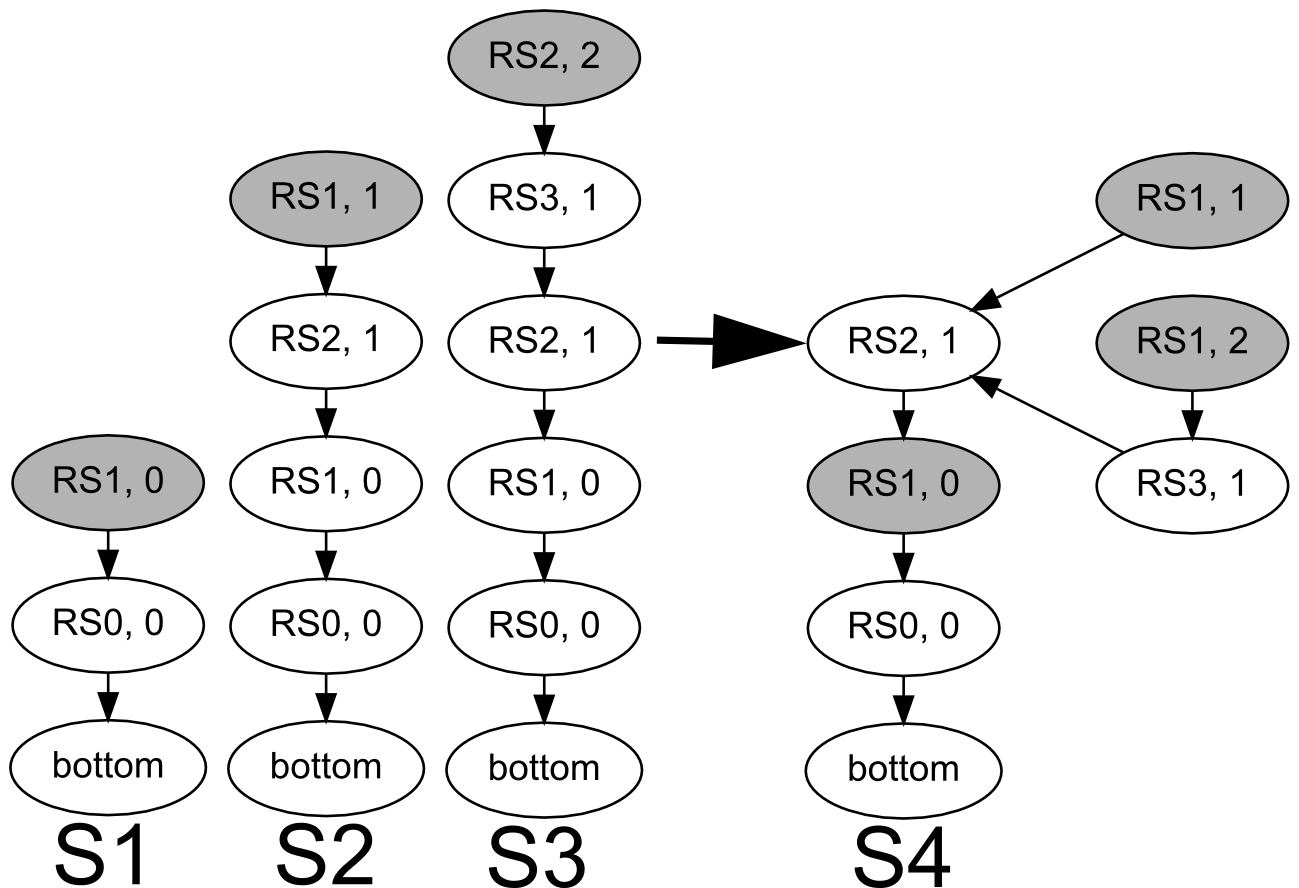
\includegraphics[width=.8\textwidth]{pics/ex_gss.png}
\caption{Пример GSS}
\label{fig:gss} 
\end{center}
\end{figure}

\subsection{Сжатое представление леса разбора}

Для переиспользования общих поддеревьев вывода Ян Рекерс (Jan Rekers, University of Amsterdam) предложил сжатое представление леса разбора (Shared Packed Parse Forest, SPPF)~\cite{SPPF}, которое позволяет компактно представлять множество деревьев вывода. Важным свойством SPPF является то, что из него можно извлечь только те и только те деревья, которые могли быть получены в результате построения вывода конкретного входа в заданной грамматике. Для обеспечения этого свойства в SPPF, кроме терминальных и нетерминальных узлов, добавляются дополнительные узлы различных типов. Конкретный набор типов дополнительные узлов может отличаться в зависимости от алгоритма анализа.

\fvset{frame=lines,framesep=5pt}
\begin{listing}
% * <Екатерина Вербицкая> 17:30:32 02 Jul 2015 UTC+0300:
% Ты вроде вводил правила как нечто со стрелкой, так и выдерживай стиль дальше в тексте.
    \begin{pyglist}[numbers=left,numbersep=5pt]

s ::= m 
s ::= p
p ::= A n
m ::= A l
l ::= n
n ::= B C

\end{pyglist}
\caption{Грамматика $G_1$}
\label{lst:g1}
\end{listing}


Пример SPPF для грамматики $G_1$ (листинг~\ref{lst:g1}) и входа \verb|ABC| приведён на рисунке~\ref{fig:ex_sppf}. Представлены два различных дерева вывода~(\ref{fig:ex_sppf1} и ~\ref{fig:ex_sppf2}) и результат их объединения в SPPF~\ref{fig:ex_sppf3}. Узлы с именами вида ``n <name>'' --- это нетерминальные узлы, ``е <name>'' --- терминальные, ``prod <num>'' --- дополнительные узлы, показывающие, согласно какой продукции из грамматики прозводился вывод нетерминала, являющегося предком данного узла.  

\begin{figure}[h!]
\centering
   \begin{subfigure}[b]{0.3\textwidth}
       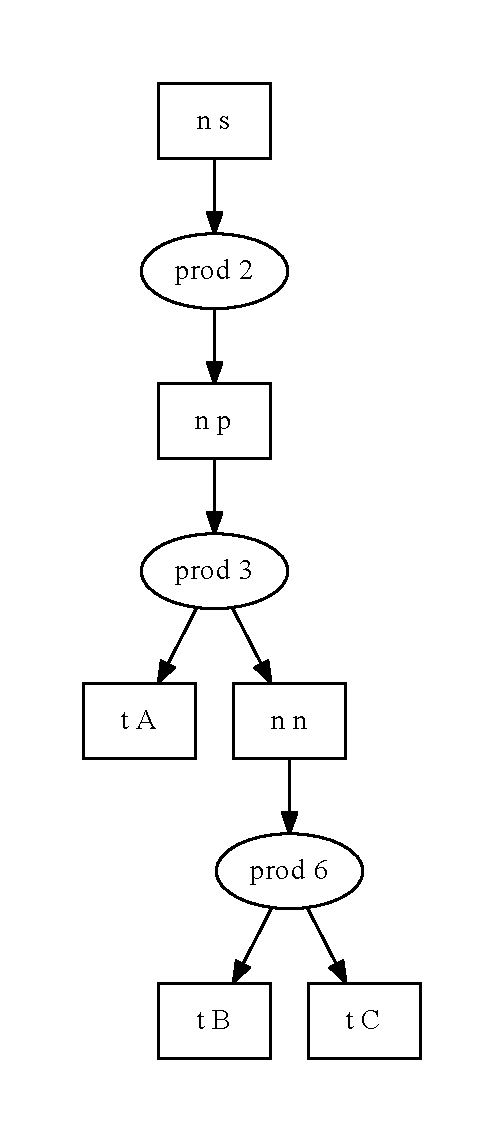
\includegraphics[width=\textwidth]{pics/ex_sppf1}
       \caption{Первое дерево вывода}
       \label{fig:ex_sppf1}
   \end{subfigure}
   ~ 
   \begin{subfigure}[b]{0.3\textwidth}
       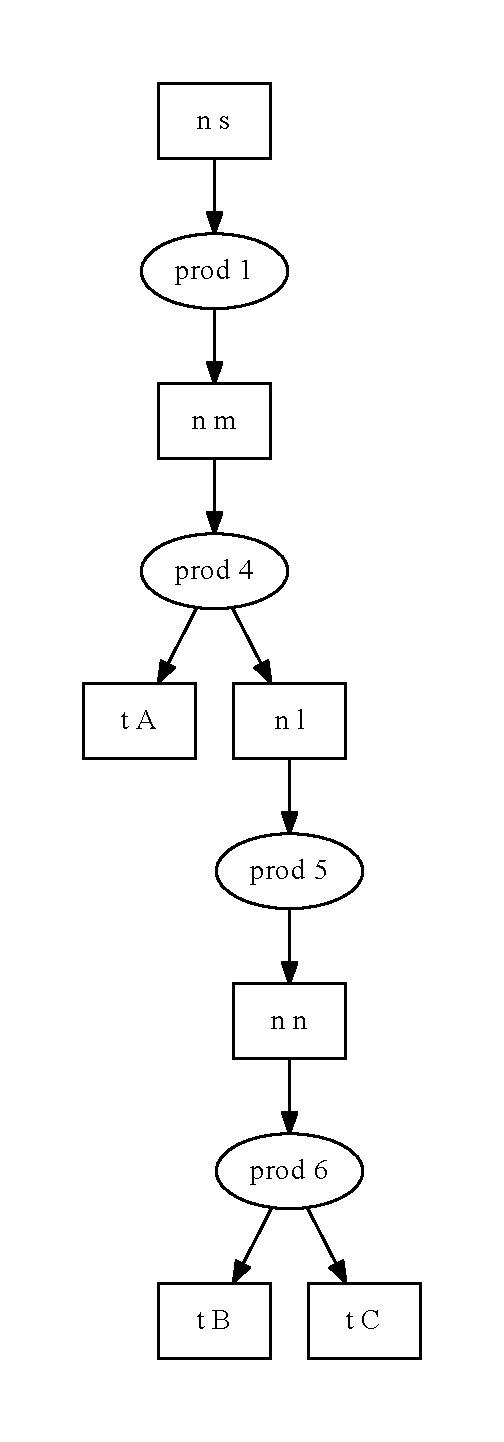
\includegraphics[width=\textwidth]{pics/ex_sppf2}
       \caption{Второе дерево вывода}
       \label{fig:ex_sppf2}
   \end{subfigure}
   ~
   \begin{subfigure}[b]{0.3\textwidth}
       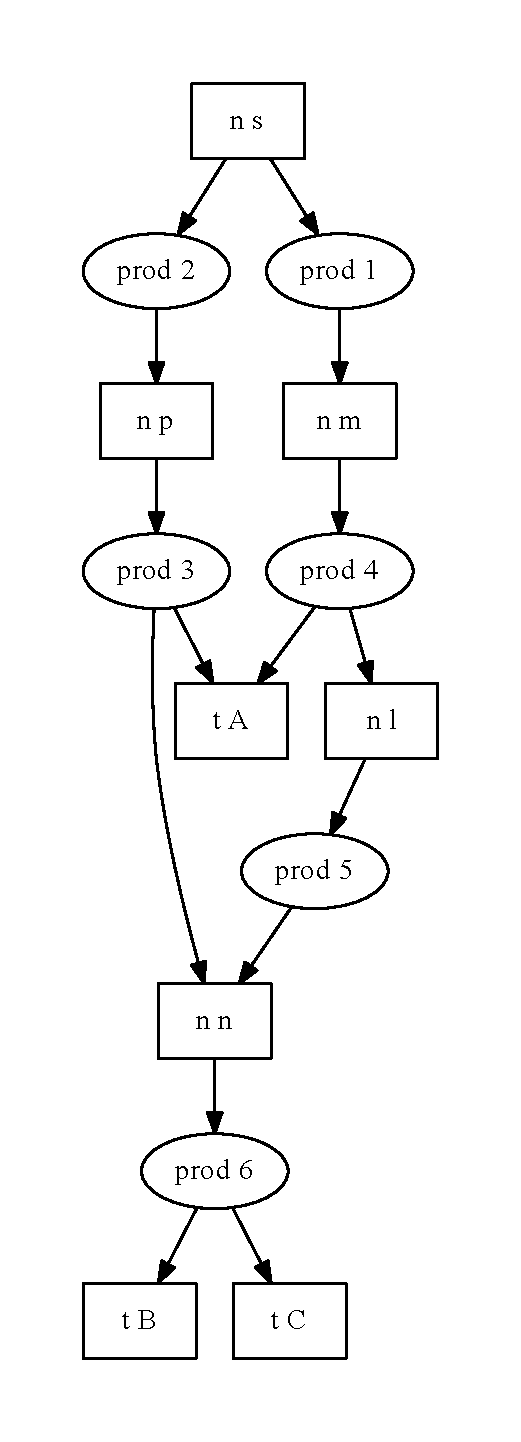
\includegraphics[width=\textwidth]{pics/ex_sppf3}
       \caption{Объединение деревьев вывода в SPPF}
       \label{fig:ex_sppf3}
   \end{subfigure}
   \caption{Пример SPPF для грамматики $G_1$ и входа \textbf{\texttt{ABC}}}
   \label{fig:ex_sppf} 
\end{figure}

\subsection{Алгоритм RNGLR}

RNGLR-алгоритм (Right-Nulled Generalized LR)~\cite{RNGLR} является модификацией предложенного Масару Томитой алгоритма, который не был способен обрабатывать все контекстно-свободные грамматики. Чтобы устранить данный недостаток, Элизабет Скотт (Elizabeth Scott) и Адриан Джонстон (Adrian Johnstone) из университета Royal Holloway (Великобритания) предложили RNGLR-алгоритм, который расширяет GLR-алгоритм специальным способом обработки обнуляемых справа правил (right-nullable rules, имеющих вид $\mathrm{A} \rightarrow \alpha \beta$, где $\beta$ выводит пустую строку $\epsilon$), позволяя обрабатывать произвольные контекстно-свободные грамматики. Алгоритм синтаксического анализа динамически формируемых выражений, представленный в данной работе, основан на RNGLR-алгоритме. Его подробное описание в виде псевдокода приведено ниже.

\begin{listing}[!ht]
\hrule
\begin{algorithmic}[1]
%\caption{RNGLR-алгоритм}
%\label{rnglr}
\Function{parse}{$grammar, input$}
  \State{$\mathcal{R} \gets \emptyset$} \Comment{Очередь троек: вершина GSS, нетерминал, длина свёртки}
  \State{$\mathcal{Q} \gets \emptyset$} \Comment{Коллекция пар: вершина GSS, состояние синтаксического анализатора}
  \If{$input = \epsilon$}
    \If{$grammar$ accepts empty input} {report success}
    \Else { report failure}
    \EndIf
  \Else
    \State{\Call{addVertex}{$0, 0, startState$}}
    \ForAll{$i$ in $0..input.Length-1$}
      \State{\Call{reduce}{$i$}}
      \State{\Call{push}{$i$}}
    \EndFor
    \If{$i=input.Length-1$ and there is a vertex in the last level of GSS which state is accepting}
      \State{report success}
    \Else { report failure}
    \EndIf
  \EndIf
\EndFunction
\Function{reduce}{$i$}
  \While{$\mathcal{R}$ is not empty}
    \State{$(v, N, l) \gets \mathcal{R}.Dequeue()$}
    \State{find the set $\mathcal{X}$ of vertices reachable from $v$ along the path of length $(l-1)$}
    \State{or length $0$ if $l=0$}
    \ForAll{$v_{h} = (level_{h}, state_{h})$ in $\mathcal{X}$}
      \State{$state_{t} \gets$ calculate new state by $state_{h}$ and nonterminal $N$}
      \State{\Call{addEdge}{$i, v_{h}, v.level, state_{tail}, (l=0)$}}
    \EndFor
  \EndWhile
\EndFunction
\Function{push}{$i$}
  \State{$\mathcal{Q^{'}} \gets$ copy $\mathcal{Q}$}
  \While{$\mathcal{Q^{'}}$ is not empty}
    \State{$(v, state) \gets \mathcal{Q}.Dequeue()$}
    \State{\Call{addEdge}{$i, v, v.level + 1, state, false$}}
  \EndWhile
\EndFunction
\end{algorithmic}
\hrule
  \caption{Критерии сравнения инструментов анализа динамически формируемых строковых выражений}\label{lst:metricsForComparison}
\end{listing}

\begin{listing}[!ht]
\hrule

\begin{algorithmic}[1]
\caption{Построение GSS}
\label{RNGLRMain}
\Function{addVertex}{$i, level, state$}
  \If{GSS does not contain vertex $v = (level, state)$}
    \State{add new vertex $v = (level, state)$ to GSS}
    \State{calculate the set of shifts by $v$ and the $input[i+1]$ and add them to $\mathcal{Q}$}
    \State{calculate the set of zero-reductions by $v$ and the $input[i+1]$ and}
    \State{add them to $\mathcal{R}$}
  \EndIf
  \State{\Return{$v$}}
\EndFunction
\Function{addEdge}{$i, v_{h}, level_{t}, state_{t}, isZeroReduction$}
  \State{$v_{t} \gets$ \Call{addVertex}{$i, level_{t}, state_{t}$}}
  \If{GSS does not contain edge from $v_{t}$ to $v_{h}$}
    \State{add new edge from $v_{t}$ to $v_{h}$ to GSS}
    \If{not $isZeroReduction$}
      \State{calculate the set of reductions by $v$ and the $input[i+1]$ and}
      \State{add them to $\mathcal{R}$}
    \EndIf
  \EndIf
\EndFunction
\end{algorithmic}

\hrule
\end{listing}

Для эффективного представления множества стеков во время синтаксического анализа в алгоритме RNGLR, как и в классическом GLR, используется структурированный в виде графа стек (GSS). Вершина GSS~--- это пара $(s,l)$, где $s$~--- состояние синтаксического анализатора, а $l$~--- уровень (позиция во входном потоке).

RNGLR-алгоритм последовательно считывает символы входного потока слева направо, по одному за раз, и строит GSS по ``слоям'': сначала осуществляются все возможные свёртки для данного символа, после чего сдвигается следующий символ со входа. Свёртка или сдвиг модифицируют GSS следующим образом. Предположим, что в GSS необходимо добавить ребро $(v_t,v_h)$. По построению, конечная вершина добавляемой дуги к такому моменту уже обязательно находится в GSS. Если начальная вершина также содержится в GSS, то в граф добавляется новое ребро (если оно ранее не было добавлено), иначе создаются и добавляются в граф и начальная вершина, и ребро. Каждый раз, когда создаётся новая вершина $v=(s,l)$, алгоритм вычисляет новое состояние синтаксического анализатора $s'$ по $s$ и следующему символу входного потока. Пара $(v,s')$, называемая push, добавляется в глобальную коллекцию $\mathcal{Q}$. Также при добавлении новой вершины в GSS вычисляется множество $\epsilon$-свёрток, после чего элементы этого множества добавляются в глобальную очередь $\mathcal{R}$. Свёртки длины $l>0$ вычисляются и добавляются в $\mathcal{R}$ каждый раз, когда создаётся новое (не-$\varepsilon$) ребро. Подробное описание работы со структурированным в виде графа стеком GSS пердставлено в листинге~\ref{RNGLRMain}.

В силу неоднозначности грамматики входная строка может иметь несколько деревьев вывода, как правило, содержащих множество идентичных поддеревьев. Для того, чтобы компактно хранить множество деревьев вывода, используется SPPF, являющееся ориентированным графом и в данном случае обладающее следующей структурой.
\begin{enumerate}
  \item \emph{Корень} соответствует стартовому нетерминалу грамматики.
  \item \emph{Терминальные} вершины, не имеющие исходящих дуг, соответствуют либо терминалам грамматики, либо деревьям вывода пустой строки $\varepsilon$.
  \item \emph{Нетерминальные} вершины являются корнем дерева вывода некоторого нетерминала грамматики; только вершины-продукции могут быть непосредственно достижимы из таких вершин.
  \item \emph{Вершины-продукции}, представляющие правую часть правила грамматики для соответствующего нетерминала. Вершины, непосредственно достижимые из них, упорядочены и могут являться либо терминальными, либо нетерминальными вершинами. Количество таких вершин лежит в промежутке $[l-k \dots l]$, где $l$~--- это длина правой части продукции, а $k$~--- количество финальных символов, выводящих $\varepsilon$. При этом такие символы игнорируются для уменьшения потребления памяти.
\end{enumerate}

SPPF создаётся параллельно с построением GSS. С каждым ребром GSS ассоциирован либо терминальный, либо нетерминальный узел. Когда добавление ребра в GSS происходит во время операции push, новая терминальная вершина создаётся и ассоциируется с ребром. Нетерминальные вершины ассоциируются с рёбрами, добавленными во время операции reduce. Если ребро уже есть в GSS, к ассоциированной с ним нетерминальной вершине добавляется новая вершина-продукция. Подграфы, ассоциированные с рёбрами пути, вдоль которого осуществлялась свёртка, добавляются как дети к вершине-продукции. После того, как входной поток прочитан до конца, производится поиск всех вершин, имеющих принимающее состояние анализатора, после чего подграфы, ассоциированные с исходящими из таких вершин рёбрами, объединяются в один граф. Из полученного графа удаляются все недостижимые из корня вершины, в результате чего остаются только корректные деревья разбора для входной строки. 

Листинг~\ref{rnglr} представляет более детальное описание алгоритма.

    
\section{Используемые инструменты}

В этом разделе описываются основные инструменты, использованные в работе: YaccConstructor~\cite{YCArticle, YCUrl}, выбранный в качастве основы для реализации алгоритма синтаксического анализа динамически формируемых выражений, и ReSharper SDK~\cite{ReSharperSDK}, использованный для разработки сшиений для microsoft Visual Studio IDE.  

\subsection{YaccConstructor}\label{YCDescr}

    Одной из задач данной работы является создание инструментария, упрощающего разработку целевых инструментов статического анализа строковых выражений, которые включают такие этапы, как лексический и синтаксический анализ. При создании лексических и синтаксических анализаторов широко распространённой практикой является использование генераторов, которые по описанию языка строят соответствующий анализатор. Данный подход должен быть реализован и для создания инструментов анализа встроенных языков.
    Работа с описаниями языков программирования --- грамматикой и лексический спецификацией --- в рамках решаемой задачи аналогична работе с ними в стандартных генераторах. По этой причине необходимо было выбрать готовую платформу для работы с грамматиками и создания синтаксических и лексических анализаторов.

        В качестве такой платформы был выбран исследовательский проект лаборатории языковых инструментов JetBrains YaccConstructor (YC)~\cite{YCArticle, YCUrl}, который является модульной платформой с открытым исходным кодом для исследований в области лексического и синтаксического анализа и разработки соответствующих инструментов. YC реализован на платформе Microsoft .NET\footnote{Microsoft .NET --- платформа для разработки программных продуктов компании Microsoft. Общие сведения о платформе: \url{https://msdn.microsoft.com/ru-ru/library/zw4w595w(v=vs.110).aspx} (Посещено 23.06.2015.)}, основной язык разработки --- F\#\footnote{F\# --- функциональный язык программирования для платформы .NET. Информация о языке: \url{http://fsharp.org} (Посещено 23.06.2015.)}~\cite{FSharp}.

\begin{figure}[h!]
\begin{center}
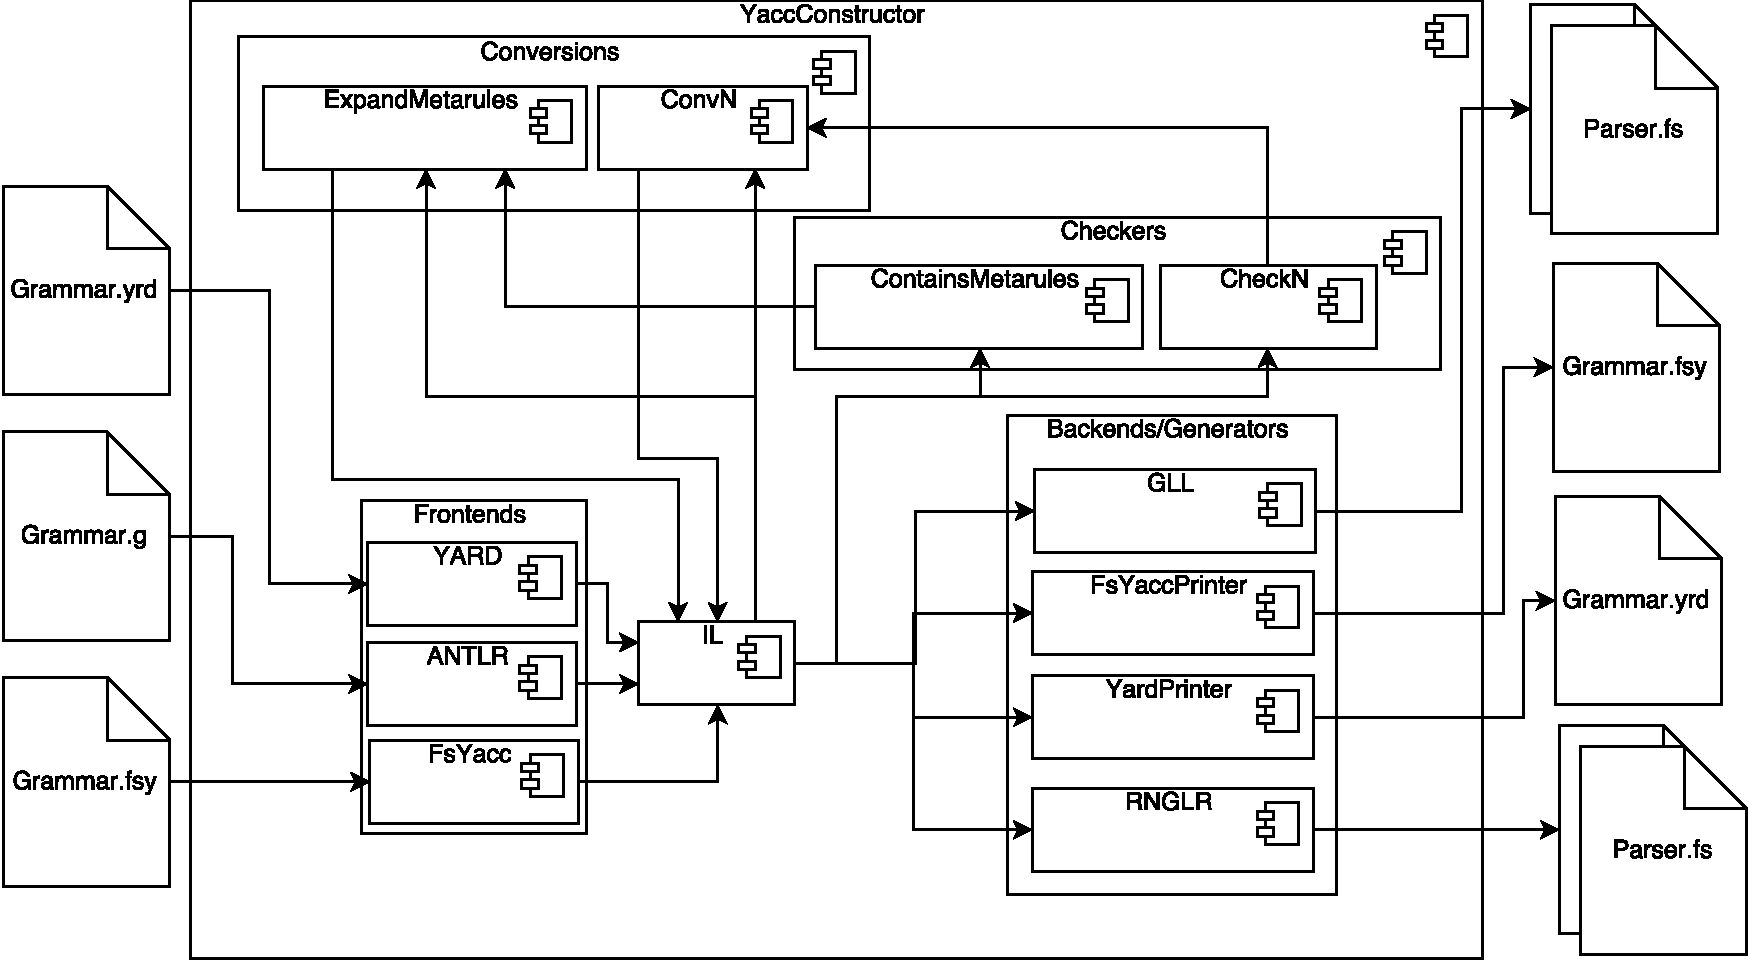
\includegraphics[width=\textwidth]{pics/YCArch.pdf}
\caption{Архитектура платформы YaccConstructor}
\label{fig:ycarch} 
\end{center}
\end{figure}

        
    Архитектура YC, представленная на рисунке~\ref{fig:ycarch}, позволяет собирать требуемый инструмент из существующих модулей: можно выбрать фронтенд, соответствующий используемому языку спецификации грамматики, задать необходимые преобразования грамматики, указать необходимый генератор. Генераторы (backend) представляют различные инструменты, которые по внутреннему представлению грамматики получают результ, полезный для конечного пользователя. Например, это могут быть генераторы синтаксических анализаторов, основанные на различных алгоритмах или принтеры, генерирующие текст грамматики в определённом формате или на заданном языке. YC является расширяемой платформой: модуль любого типа может быть реализован, в том числе с переиспользованием уже существующих, и подключён к платформе.  

    В рамках YC разработан выразительный язык спецификации грамматик YARD, поддерживающий атрибутные грамматики, грамматики в EBNF~\footnote{EBNF --- расфиренная форма Бэкуса-Наура. Грамматики в этой форме позволяют использовать регулярные выражения в правых частях правил~\cite{EBNFISO}.} и многое другое. В листинге~\ref{lst:calcExample} представлена грамматика языка арифметических выражений Calc на языке YARD.  

\fvset{frame=lines,framesep=5pt}
\begin{listing}
    \begin{pyglist}[numbers=left,numbersep=5pt]
    
    [<Start>]
    expr: factor [MULT expr]
    powExpr: NUM | LBR expr RBR
    factor: powExpr [POW factor]
    
\end{pyglist}
\caption{Пример грамматики языка арифметических выражений на языке YARD}
\label{lst:calcExample}
\end{listing}


    Выразительный синтаксис языка описания грамматики удобен для разработчика, однако генераторы, как правило, не поддерживают обработку грамматик в таком виде. Часто требуется, чтобы правая часть правила  грамматики не содержала регулярных выражений, а состояла бы из цепочки из терминалов и нетерминалов. Это необходимо для работы алгоритма построения таблиц. Для решения этой задачи в YC реализован ряд преобразований грамматик. В результате их применения к грамматике, представленной в листинге~\ref{lst:calcExample}, можно получить грамматику, представленную в листинге~\ref{lst:calcTransformExample}.


\fvset{frame=lines,framesep=5pt}
\begin{listing}
    \begin{pyglist}[numbers=left,numbersep=5pt]
    
    [<Start>]
    expr: factor 
    expr: factor MULT expr
    powExpr: NUM 
    powExpr: LBR expr RBR
    factor: powExpr
    factor: powExpr POW factor
    startRule: expr

\end{pyglist}
\caption{Пример преобразованной грамматики языка арифметических выражений}
\label{lst:calcTransformExample}
\end{listing}

    Также в рамках платформы YC в качестве одного из модулей ранее был реализован генератор синтаксических анализаторов на основе RNGLR-алгоритма. Это позволяет переиспользовать общие функции и структуры данных при разработке анализатора для встроенных языков. 
    Таким образом, алгоритм анализа встроенных языков и соответствующий генератор может быть реализован в рамках платформы YC в качестве одного из модулей. При этом можно использовать готовый язык описания грамматики и преобразования, а также переиспользовать необходимые элементы генератора анализаторов на основе RNGLR-алгоритма. Таким образом, YC был выбран в качестве основы для реализации благодаря удобной архитектуре и большому количеству готовых решений. 


\subsection{ReSharper SDK}\label{ReSharperSDKDescr}

    Для демонстрации разработанного в рамках данной работы инструмента представляется целесообразным создать на его основе целевое решение. Для этого необходимо окружение, способное обрабатывать внешний язык, поскольку такие операции над внешним языком, как построение дерева разбора, базовый анализ (например, построение графа потока управления или графа потока данных), лежат за пределами рассматриваемой в данной работе задачи, и их выполнение должно осуществляться сторонними инструментами. При этом такие инструменты должны предоставлять необходимую для решения основной задачи функциональность. Кроме того, необходимо иметь удобный способ взаимодействия с пользователем: необходимо получать код для анализа и отображать результаты в виде, удобном для пользователя. Один из самых распространённых способов работы с программным кодом --- это работа в интегрированной среде разработки.

    Так как реализация работы велась на платформе Microsoft .NET, то соответствующее окружение для обработки внешнего языка и организации взаимодействия с пользователем на данной платформе должно работать на данной платформе. Одной из самых известных сред разработки для платформы .NET, позволяющей создавать расширения на .NET языках, является Microsoft Visual Studio IDE\footnote{Сайт среды разработки Microsoft Visual Studio IDE: \url{https://www.visualstudio.com/} (Посещён 23.06.2015.)}. Она и была выбрана в качестве цели для интеграции инструмента статического анализа строковых выражений. Однако у данной среды разработки достаточно сложный механизм создания расширений, что вызвано его универсальностью. При решении нашей задачи универсальность не требовалась, поэтому можно было бы использовать менее универсальный и более простой механизм.

Такой механизм предоставляется ReSharper SDK~\cite{ReSharperSDK}.  ReSharper~\cite{ReSharper} --- расширение для Microsoft Visual Studio, предоставляющее пользователю широкий набор дополнительных анализов кода. Для разработчиков предоставляется свободно распространяемая SDK, реализующая анализ таких языков, как C\#, VB.NET и др. Большая часть функциональности ReSharper выделена в свободно распространяемую SDK, что даёт возможность сторонним разработчикам создавать собственные расширения к ReSharper, переиспользуя его функциональность. В контексте данной работы это позволяет упростить создание плагинов для поддержки различных встроенных языков. Кроме того, ReSharper SDK предоставляет более удобную ``обёртку'' над многими интерфейсами Microsoft Visual Studio, что упрощает взаимодействие с ней и полезно, например, при предоставлении результатов пользователю.

Следует также отметить, что ReSharper является многоязыковым инструментом, то есть поддерживает большой набор различных языков и спроектирован так, чтобы максимально упростить поддержку новых языков. Это позволяет создавать инструменты, обрабатывающие не только различные встроенные языки, но также и различные внешние.

 Выделим следующую функциональность ReSharper SDK, необходимую для реализации поддержки встроенных языков в Microsoft Visual Studio.  
\begin{itemize}
    \item Построение дерева разбора внешнего языка (C\#, JavaScript и другие, поддерживаемые ReSharper), узлы которого содержат координаты в исходном коде, что позволяет точно связывать текстовое и структурное представление кода.
    \item Анализ потока данных и анализ потока управления для поддерживаемых языков. На основе существующих анализов можно строить более сложные, необходимые, например, для построения регулярной аппроксимации.
    \item Вывод сообщений об ошибках и графическое выделение некорректных мест в текстовом редакторе.
    \item Взаимодействие с редактором кода, позволяющее настраивать подсветку синтаксиса, получать позицию курсора и управлять ею, что нужно для динамической подсветки парных элементов.
\end{itemize}

Таким образом ReSharper SDK и Microsoft Visual Studio IDE выбраны в качестве основы для разработки целевого инструмента на основе представленных в данной работе результатов.

\section{Выводы}

На основе проведённого обзора можно сделать следующие выводы, обосновывающие необходимость проведения исследований в области статического анализа динамически формируемых строковых выражений.

\begin{itemize}
    \item Проблема анализа строковых выражений актуальна в нескольких областях: поддержка встроенных языков в интегрированных средах разработки, оценка качества кода, содержащего динамически формируемые строковые выражения, реинжиниринг программного обеспечения.
    \item Большинство реализаций поддерживают конкретный внешний и конкретный встроенный язык и, как правило, решают одну достаточно узкую задачу. При этом, зачастую, плохо расширяемы, как в смысле поддержки других языков, так и в смысле решения новых задач. Полноценные средства разработки инструментов статического анализа динамически формируемых выражений, упрощающие создание решений для новых языков, отсутствуют.
    \item Для эффективного решения этих задач необходимо структурное представление кода, однако на текущий момент не представлено законченного решения, позволяющего строить деревья вывода для динамически формируемых выражений.
\end{itemize}

Кроме того, обзор позволяет выявить следующие подходы, технологии и средства.

\begin{itemize}
    \item В качестве приближения множества значений целесообразно использовать регулярную аппроксимацию~\cite{JSA, RegOverApprox}, так как при работе с ней ряд важных задач является разрешимым в общем случае, что не верно для контекстно-свободной. Более того, работа с регулярной аппроксимацией упрощает решение такой задачи, как лексический анализ встроенных языков.
    \item Лексический и синтаксический анализы должны быть разделены. Это оправдано как с теоретической, так и с практической точек зрения, так как лексический анализ не привносит потери точности и упрощается переиспользование спецификаций языков и самих анализаторов. 
    \item В качестве основы алгоритма синтаксического анализа днамически формируемых выражений можно выбрать алгоритм обобщённого синтаксического анализа~\cite{GeneralisedlrBIG}, так как в нём реализовано эффективное управление множеством стеков и деревьев разбора, что важно при работе с динамически формируемыми выражениями.
\end{itemize}
\clearpage

\chapter{Алгоритм синтаксического анализа регулярной аппроксимации} \label{relWorks}

В данной главе будет формально описана решаемая задача синтаксического анализа динамически формируемых выражений, изложен алгоритм её решения. Также будут сформулированы и доказаны утверждения о корректности изложенного алгоритма.

\section{Постановка задачи}
% * <Екатерина Вербицкая> 12:39:59 01 Jul 2015 UTC+0300:
% Уверен, что такое название подраздела приемлемо?

Анализируемая программа $\mathcal{P}$ является генератором выражений и таким образом задаёт некоторый язык $L_1$. Предположим, что $\mathcal{P}$ взаимодействует с базой данных с помощью динамически формируемых выражений. В этом случае мы говорим, что $\mathcal{P}$ использует динамический SQL, подразумевая, что программой генерируются выражения на языке SQL. Однако это не совсем корректно, так как программа может, например, содержать ошибку и некоторые из построенных ей выражений не будут корректными SQL-выражениями. Таким образом, в этом случае $L_1\neq$~SQL.

С другой стороны, может быть задан эталонный язык $L_2$ --- язык, которому должны принадлежать все выражения генерируемые программой $\mathcal{P}$. Как правило $L_2$ описывается с помощью контекстно-свободной грамматики. Например, это может быть грамматика конкретного диалекта SQL, взятая из документации.

В результате мы имеем описание двух языков и задача проверки корректности выражений, генерируемых $\mathcal{P}$, может быть сформулирована как проверка вложенности языка $L_1$ в язык $L_2$. Однако в рамках данной работы нас интересует не просто вложенность языков, а построение деревьев вывода. Как уже говорилось, язык $L_2$ может быть задан с помощью грамматики. Пусть задана грамматика $G$, такая, что $L_2 = L(G)$, тогда задача синтаксического анализа динамически формируемых выражений может быть поставлена следующим образом: для всех цепочек $\omega \in L_1$, выводимых в грамматике $G$, построить соответствующие деревья вывода.

Отметим, что решение изложенных выше вопросов в общем виде возможно не всегда. Трудности могут быть связаны прежде всего с классами рассматриваемых языков. Эталонный язык $L_2$, скорее всего, является некоторым языком программирования и принадлежит к классу контекстно-свободных языков (хотя могут быть и исключения). Генерируемый язык $L_1$, вообще говоря, не обязан быть даже контекстно-зависимым. Так как программа-генератор реализована на тьюринг-полном языке, то $L_1$ в общем случае может быть рекурсивно-перечислимым. Из практических соображений хочется думать, что $L_1$ всё же является подмножеством некоторого языка программирования и может быть достаточно хорошо приближен некоторым контекстно-свободным языком. Однако проверка включения двух контекстно-свободных языков не разрешима в общем случае~\ref{!!!!}. При этом точно разрешима в общем случае проверка включения регулярного языка в однозначный контекстно-свободный~\ref{!!!!}. В однозначные КС языки попадают такие практически значимые классы, как LR(k) и LL(k), что позволяет использовать в качестве $L_2$ практически значимые языки. Для $L_1$ же необходимо строить регулярное приближение $L_R$.

Чтобы обеспечить надёжность анализа строковых выражений, необходимо, чтобы приближение было сверху. Нам нужна аппроксимация сверху, то есть должно выполняться включение $L_1 \subseteq L_R$. Это необходимо для того, чтобы не потерять информацию об анализируемом языке. Например, при работе со встроенным SQL безопаснее считать таблицу используемой, чем удалить её как неиспользуемую, если она на самом деле использовалась. При этом необходимо следить за точностью такой аппроксимации, чтобы избегать слишком большого количества ошибок. В работе~\ref{!!!!} показано, как можно строить достаточно точную регулярную аппроксимацию сверху с учётом строковых операций и циклов.

Таким образом, далее мы будем предполагать, что язык $L_2$ является однозначным контекстно-свободным и задан некоторой грамматикой $G$, а для языка $L_1$ строится регулярный язык $L_R$ такой, что $L_1 \subseteq L_R$ и мы работает далее с $L_R$. При этом основной нашей задачей является построение деревьев разбора для всех цепочек из $L_R$, корректных относительно грамматики $G$. Однако $L_R$ может быть бесконечным языком и, следовательно, содержать бесконечное множество корректных цепочек. По этой причине явное построение всех деревьев разбора не представляется возможным. Решением, возможно, будет являться структура, которая при конечном объёме будет хранить бесконечное количество деревьев. При этом деревья должны однозначно извлекаться из этой структуры. То есть из построенной структуры можно получить только те и только те деревья, которые соответствуют разбору какой-либо корректной цепочки из $L_R$ языка в эталонной грамматике $G$.

Регулярный язык $L_R$ может быть представлен в виде конечного автомата. Заметим, что непосредственно построенная аппроксимация будет являться конечным автоматом $M_1=(Q_1,\Sigma_1,\delta_1,q_{0_{1}},q_{f_{1}})$ над алфавитом символов, что не очень удобно для проведения синтаксического анализа, так как грамматика $G = \langle T, N, P, S \rangle$ задана, скорее всего, над алфавитом токенов, не равным алфавиту символов. То есть $\Sigma_1 \neq T$. Чтобы устранить эту проблему можно воспользоваться конечным преобразователем (FST), который предназначен для трансформации языков. Таким образом, можно получить конечный автомат $M_2=(Q_2,\Sigma_2,\delta_2,q_{0_{2}},q_{f_{2}})$ такой, что $\Sigma_2 \subseteq T$. Такой переход является лексическим анализом регулярной аппроксимации или встроенного языка.

Заметим так же, что без потери общности можно считать, что $M_2$ является детерминированным конечным автоматом без $\varepsilon$-переходов, так как любой конечный автомат можно преобразовать к эквивалентному детерминированному без  $\varepsilon$-переходов.

Таким образом, решаемая в данной работе задача синтаксического анализа динамически формируемых выражений будет формулироваться следующим образом. \textit{ Для данной однозначной контекстно-свободной грамматики $G = \langle T, N, P, S \rangle$ и детерминированного конечного автомата без $\varepsilon$-переходов $M_2=(Q,\Sigma,\delta,q_0,q_f)$ такого, что $\Sigma \subseteq T$, необходимо построить конечную структуру данных $F$, содержащую деревья вывода в $G$ всех цепочек $\omega \in L(M)$, корректных относительно грамматики $G$, и не содержащую других деревьев. } Иными словами, надо построить алгоритм $\mathbb{P}$ такой, что
    $$(\forall \omega \in L(M)) (\omega \in L(G) \Rightarrow (\exists t \in \mathbb{P}(L(M),G))AST(t, \omega, G))$$
    $$\land (\forall t \in \mathbb{P}(L(M),G))(\exists \omega \in L(M))AST(t,\omega,G)$$, где 
    $AST(t,\omega,G)$ --- это предикат, который истинен, если $t$ является деревом вывода $\omega$ в грамматике $G$.

% * <Andrew Ivanov> 11:21:38 01 Jul 2015 UTC+0300:
% Формула ну совсем нечитаемо выглядит. Может, имеет смысл её оформить как выключную?
Так как $\mathbb{P}$ игнорирует ошибки, то будем называть его алгоритмом \textit{ослабленного} синтаксического анализа регулярной аппроксимации динамически формируемого выражения.


\section{Описание алгоритма}

Алгоритм принимает на вход эталонную однозначную контекстно-свободную грамматику $G=\langle T, N, P, S \rangle$ над алфавитом терминальных символов $T$ и детерминированный конечный автомат $(Q,\Sigma,\delta,q_0,q_f)$, имеющий одно стартовое состояние $q_0$, одно конечное состояние $q_f$, без $\epsilon$-переходов, где $\Sigma \subseteq T$~--- алфавит входных символов, $Q$~--- множество состояний, $\delta$~--- отношение перехода. По описанию  грамматики генерируются управляющие RNGLR-таблицы и некоторая вспомогательная информация (называемая $parserSource$ в псевдокоде). 

\begin{algorithm}[!ht]
\begin{algorithmic}[1]
\caption{Алгоритм ослабленного синтаксического анализа регулярной аппроксимации динамически формируемого выражения}
\label{parsing}
\Function{parse}{$grammar, automaton$}
  \State{$inputGraph \gets$ construct inner graph representation of $automaton$}
  \State{$parserSource \gets$ generate RNGLR parse tables for $grammar$}
  \If{$inputGraph$ contains no edges}
    \If{$parserSource$ accepts empty input} {report success}
    \Else { report failure}
    \EndIf
  \Else
    \State{\Call{addVertex}{$inputGraph.startVertex, startState$}}
    \State{$\mathcal{Q}.Enqueue(inputGraph.startVertex)$}
    \While{$Q$ is not empty}
      \State{$v \gets \mathcal{Q}.Dequeue()$}
      \State{\Call{makeReductions}{$v$}}
      \State{\Call{push}{$v$}}
      \State{\Call{applyPassingReductions}{$v$}}
    \EndWhile
    \If{$\exists v_f: v_f.level = q_f$ and $v_f.state$ is accepting} {report success}
    \Else { report failure}
    \EndIf
  \EndIf
\EndFunction
\end{algorithmic}
\end{algorithm}

Алгоритм производит обход графа входного автомата и последовательно строит GSS способом, аналогичным используемому в RNGLR-алгоритме. Однако так как мы имеем дело с графом вместо линейного потока, понятие следующего символа трансформируется во \emph{множество терминальных символов}, лежащих на всех исходящих рёбрах данной вершины, что несколько изменяет операции shift и reduce (смотри строку 5 в алгоритме~\ref{processVertex} и строки 9 и 21 в алгоритме~\ref{gss_construction}). Для того чтобы управлять порядком обработки вершин входного графа, мы используем глобальную очередь $\mathcal{Q}$. Каждый раз, когда добавляется новая вершина GSS, сначала необходимо произвести все свёртки длины 0, после чего выполнить сдвиг следующих токенов со входа. Таким образом необходимо добавить соответствующую вершину графа в очередь на обработку. Добавление нового ребра GSS может порождать новые свёртки, таким образом в очередь на обработку необходимо добавить вершину входного графа, которой соответствует начальная вершина добавленного ребра. Детальное описание процесса построения GSS приведено в алгоритме~\ref{parsing}. Свёртки производятся вдоль путей в GSS, и если было добавлено ребро, начальная вершина которого ранее присутствовала в GSS, необходимо заново вычислить проходящие через эту вершину свертки (смотри функцию applyPassingReductions в алгоритме~\ref{processVertex}).

\begin{algorithm}[H]
\begin{algorithmic}[1]
\caption{Обработка вершины внутреннего графа}
\label{processVertex}
\Function{push}{$innerGraphV$}
  \State{$\mathcal{U} \gets$ copy $innerGraphV.unprocessed$}
  \State{clear $innerGraphV.unprocessed$}
  \ForAll{$v_{h}$ in $\mathcal{U}$}  
    \ForAll{$e$ in outgoing edges of $innerGraphV$}
      \State{$push \gets$ calculate next state by $v_{h}.state$ and the token on $e$}
      \State{\Call{addEdge}{$v_{h}, e.Head, push, false$}}
      \State{add $v_{h}$ in $innerGraphV.processed$}
    \EndFor
  \EndFor
\EndFunction

\Function{makeReductions}{$innerGraphV$}
  \While{$innerGraphV.reductions$ is not empty}
    \State{$(startV, N, l) \gets innerGraphV.reductions.Dequeue()$}
    \State{find the set of vertices $\mathcal{X}$ reachable from $startV$}
    \State{    along the path of length ($l-1$), or $0$ if $l=0$;}
    \State{add $(startV, N, l-i)$ in $v.passingReductions$,}
    \State{    where $v$ is an $i$-th vertex of the path}
    \ForAll{$v_{h}$ in $\mathcal{X}$}
      \State{$state_{t} \gets$ calculate new state by $v_{h}.state$ and nonterminal $N$}
      \State{\Call{addEdge}{$v_{h}, startV, state_{t}, (l=0)$}}
    \EndFor
  \EndWhile
\EndFunction

\Function{applyPassingReductions}{$innerGraphV$}
  \ForAll{$(v, edge)$ in $innerGraphV.passingReductionsToHandle$}
    \ForAll{$(startV, N, l) \gets v.passingReductions.Dequeue()$}
      \State{find the set of vertices $\mathcal{X}$,}
      \State{    reachable from $edge$ along the path of length ($l-1$)}
      \ForAll{$v_{h}$ in $\mathcal{X}$}
        \State{$state_{t} \gets$ calculate new state by $v_{h}.state$ and nonterminal $N$}
        \State{\Call{addEdge}{$v_{h}, startV, state_{t}, false$}}
      \EndFor
    \EndFor
  \EndFor
\EndFunction
\end{algorithmic}
\end{algorithm}

Так же как и RNGLR, мы ассоциируем вершины GSS с позициями входного графа, однако в нашем случае уровень вершины~--- это состояние входного автомата. Мы строим внутреннюю структуру данных (в дальнейшем изложении называемую \emph{внутренним графом}) посредством копирования графа входного автомата и связывания с его вершинами следующих коллекций.
\begin{itemize}
  \item \emph{processed}: вершины GSS, для которых ранее были вычислены все операции push. Это множество агрегирует все вершины GSS, ассоциированные с вершиной внутреннего графа.
  \item \emph{unprocessed}: вершины GSS, операции push для которых ещё только предстоит выполнить. Это множество аналогично множеству $\mathcal{Q}$ алгоритма RNGLR.
  \item \emph{reductions}: очередь, аналогичная очереди $\mathcal{R}$ RNGLR-алгоритма: все операции reduce, которые ещё только предстоит выполнить.
  \item \emph{passingReductionsToHandle}: пары из вершины GSS и ребра GSS, вдоль которых необходимо осуществлять проходящие свёртки.
\end{itemize}

\begin{algorithm}[H]
\begin{algorithmic}[1]
\caption{Построение GSS}
\label{gss_construction}
\Function{addVertex}{$innerGraphV, state$}
  \State{$v \gets$ find a vertex with state $=state$ in}
  \State{    $innerGraphV.processed \cup innerGraphV.unprocessed$}
  \If{$v$ is not $null$ } \Comment{Вершина была найдена в GSS}
    \State{\Return{($v, false$)}} 
  \Else
    \State{$v \gets$ create new vertex for $innerGraphV$ with state $state$}
    \State{add $v$ in $innerGraphV.unprocessed$}
    \ForAll{$e$ in outgoing edges of $innerGraphV$}
      \State{calculate the set of zero-reductions by $v$}
      \State{    and the token on $e$ and add them in $innerGraphV.reductions$}
    \EndFor
    \State{\Return{$(v, true$)}}
  \EndIf
\EndFunction

\Function{addEdge}{$v_{h}, innerGraphV, state_{t}, isZeroReduction$}
  \State{$(v_{t}, isNew) \gets$ \Call{addVertex}{$innerGraphV, state_{t}$}}
  \If{GSS does not contain edge from $v_{t}$ to $v_{h}$}
    \State{$edge \gets$ create new edge from $v_{t}$ to $v_{h}$}
    \State{$\mathcal{Q}.Enqueue(innerGraphV)$}
    \If{not $isNew$ and $v_{t}.passingReductions.Count>0$}
      \State{add $(v_{t}, edge)$ in $innerGraphV.passingReductionsToHandle$}
    \EndIf
    \If{not $isZeroReduction$}
      \ForAll{$e$ in outgoing edges of $innerGraphV$}
        \State{calculate the set of reductions by $v$}
        \State{    and the token on $e$ and add them in $innerGraphV.reductions$}
      \EndFor
    \EndIf
  \EndIf
\EndFunction
\end{algorithmic}
\end{algorithm}

Помимо состояния анализатора $state$ и уровня $level$ (который совпадает с состоянием входного автомата), в вершине GSS хранится коллекция \emph{проходящих свёрток}. Проходящая свёртка~--- это тройка $(startV, N, l)$, соответствующая свёртке, чей путь содержит данную вершину GSS. Аналогичная тройка используется в RNGLR-алгоритме для описания свёртки, но в данном случае $l$ обозначает длину оставшейся части пути. Проходящие свёртки сохраняются в каждой вершине пути (кроме первой и последней) во время поиска путей в функции $makeReductions$ (см. алгоритм~\ref{processVertex}).

\section{Построение компактного представления леса разбора}
В качестве компактного представления леса разбора всех корректных выражений из множества значений динамически формируемого выражения используется граф SPPF. Построение компактного представления осуществляется одновременно с синтаксическим разбором во время построения графа стеков GSS, так же как и в алгоритме RNGLR.

С каждым ребром GSS ассоциируется список лесов разбора фрагмента выражения. В графе GSS нет кратных рёбер, поэтому если во время работы функции \emph{addEdge} в нем было найдено добавляемое ребро, то с ним ассоциируется новый лес разбора, при этом в очередь на обработку не добавляется никаких вершин входного графа.  

При добавлении в GSS ребра, соответствующего считанной со входа лексеме, создаётся (и ассоциируется с ним) граф из одной терминальной вершины. Так как входной автомат является детерминированным, с ребром GSS ассоциируется не более одного такого графа.

При обработке свёртки алгоритм осуществляет поиск всех путей в графе GSS заданной длины, после чего происходит добавление в GSS новых ребер, соответствующих данной свёртке. С каждым таким ребром ассоциируется лес, имеющий в качестве корня (вершины, у которой нет входных рёбер) вершину, соответствующую нетерминалу, к которому осуществлялась свёртка. Ребра каждого из найденных путей, перечисленные в обратном порядке, образуют правую часть некоторого правила грамматики, по которому осуществляется свёртка. Для каждого пути создаётся вершина, помеченная номером такого правила, и добавляется в лес как непосредственно достижимая из корня. Каждое ребро пути ассоциировано со списком лесов вывода символа из правой части правила. Непосредственно достижимыми вершинами вершины-правила становятся ссылки на такие списки, за счёт чего осуществляется переиспользование фрагментов леса.

В алгоритме RNGLR наличие нескольких путей, вдоль которых осуществляется свёртка к нетерминалу, означает существование более чем одного варианта вывода нетерминала. В нашем случае данная ситуация соответствует различным фрагментам нескольких выражений из входного регулярного множества, которые сворачиваются к одному нетерминалу. 

В конце работы алгоритма осуществляется поиск ребер GSS, для каждого из которых верно, что конечная вершина имеет уровень, равный финальному состоянию входного автомата, и принимающее состояние (accepting state). Результирующее представление леса разбора получается путём удаления недостижимых вершин из графа, созданного объединением лесов разбора, ассоциированных с найденными рёбрами GSS.

Рассмотрим фрагмент кода, представленный в листинге~\ref{lst:brExpr}, который динамически формирует выражение expr в строке 4.

\fvset{frame=lines,framesep=5pt}
\begin{listing}
\begin{pyglist}[language=csharp,numbers=left,numbersep=5pt]
 string expr = "" ;
 for(int i = 0; i < len; i++) 
 {
     expr = "()" + expr;
 }
\end{pyglist}
\caption{Пример кода на языке программирования C\#, динамически формирующего скобочную последовательность}
\label{lst:brExpr}
\end{listing}

Множество значений выражения \textbf{\texttt{expr}} аппроксимируется регулярным выражением $(\mbox{\texttt{LBR }} \mbox{\texttt{RBR}})*$, где $\mbox{\texttt{LBR }}$ соответствует открывающейся скобке, а $\mbox{\texttt{RBR}}$~--- закрывающейся. Граф конечного автомата, задающего такую аппроксимацию, изображён на рисунке~\ref{input}.

\begin{figure}[!h]
 \centering
 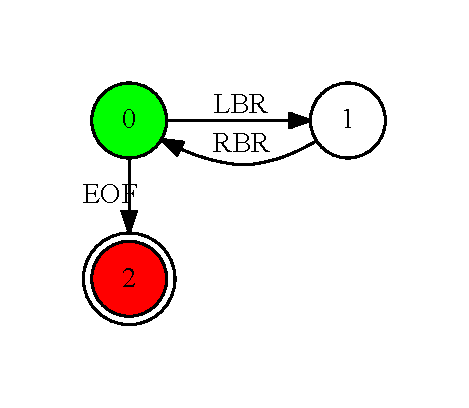
\includegraphics[]{pics/input.pdf}
 \caption{Конечный автомат, задающий регулярную аппроксимацию выражения \textbf{\texttt{expr}}}
 \label{input}
\end{figure}

В результате работы предложенного алгоритма будет получено конечное представление леса разбора SPPF, изображённое на рисунке~\ref{sppf}.

\begin{figure}[!h]
 \centering
 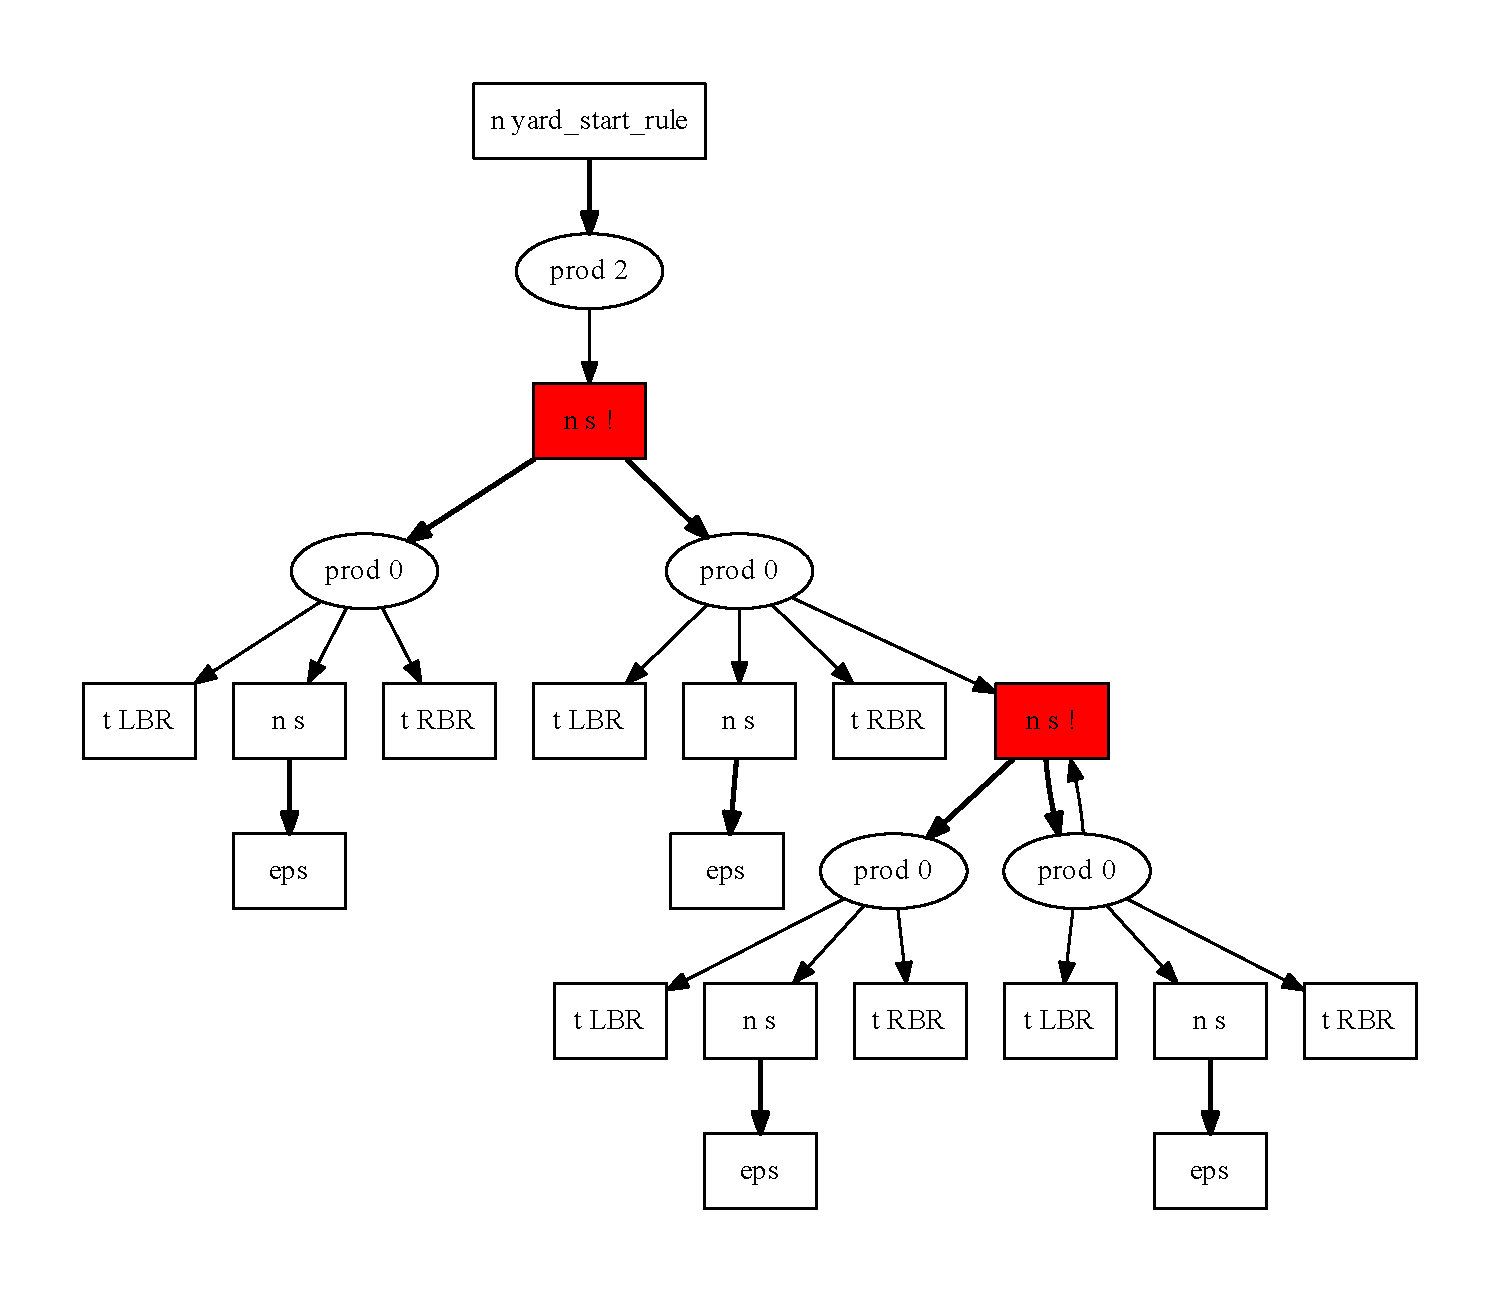
\includegraphics[width=.9\textwidth]{pics/sppf.pdf}
 \caption{Конечное представление леса разбора для выражения \textbf{\texttt{expr}}}
 \label{sppf}
\end{figure}

\begin{figure}[!h]
 \centering
 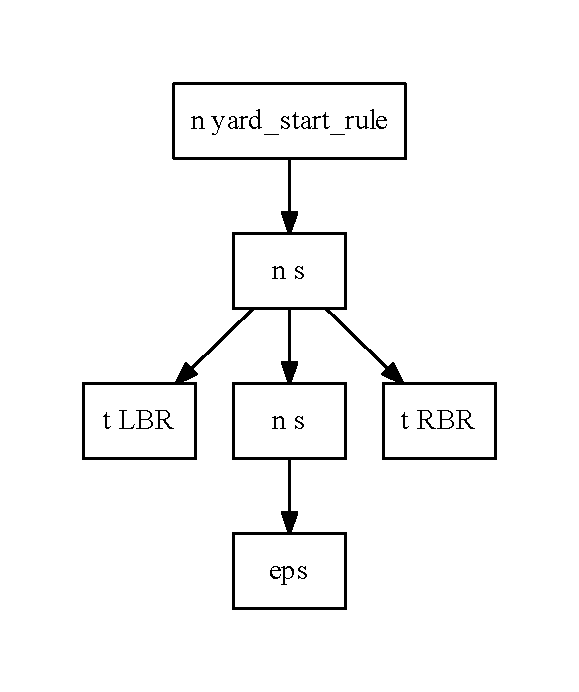
\includegraphics[width=.4\textwidth]{pics/sppf1.pdf}
 \caption{Дерево вывода для выражения $expr="()"$}
 \label{sppf1}
\end{figure}

\begin{figure}[!h]
 \centering
 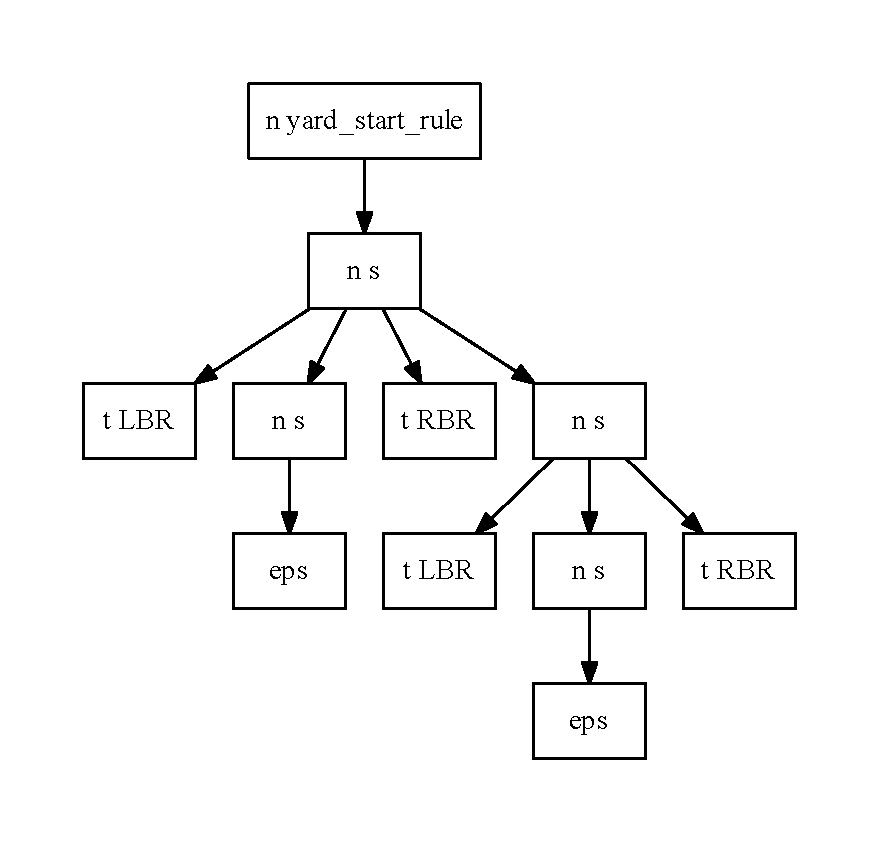
\includegraphics[width=.6\textwidth]{pics/sppf2.pdf}
 \caption{Дерево вывода для выражения $expr="()()"$}
 \label{sppf2}
\end{figure}

\begin{figure}[!h]
 \centering
 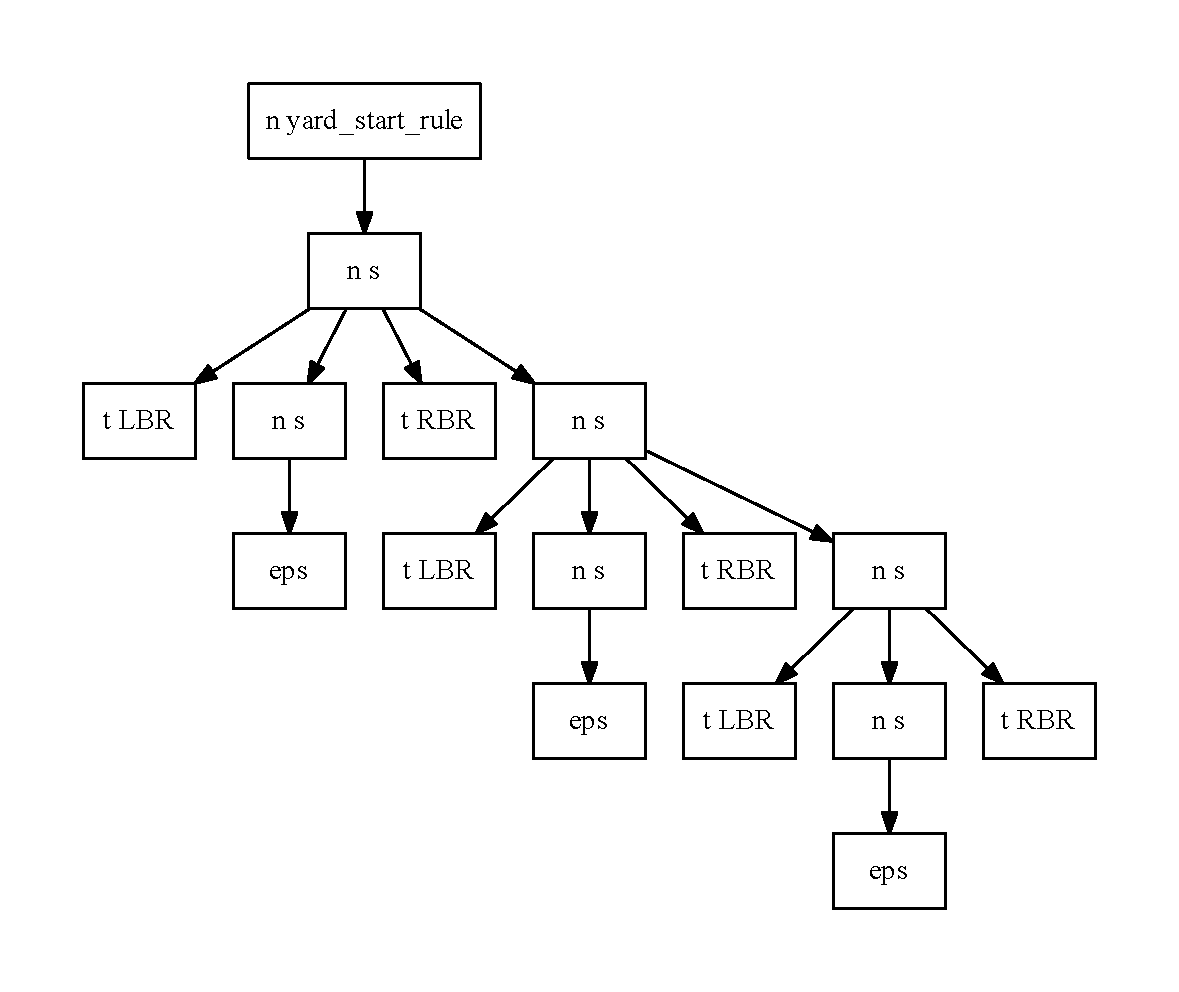
\includegraphics[width=.6\textwidth]{pics/sppf3.pdf}
 \caption{Дерево вывода для выражения $expr="()()()"$}
 \label{sppf3}
\end{figure}

Из построенного SPPF можно извлечь бесконечное количество деревьев, каждое из которых является деревом вывода некоторой цепочки из регулярной аппроксимации. На серии рисунков~\ref{sppf1,sppf2,sppf3} представлены извлечённые деревья разбора для различных значений выражения \textbf{\texttt{expr}}.  

\chapter{Доказательство корректности алгоритма}
\textsc{Теорема 1.} 
\textit{Алгоритм завершает работу для любых входных данных.}

\textsc{Доказательство.}
С каждой вершиной внутреннего представления графа входного конечного автомата ассоциировано не более $N$ вершин графа GSS, где $N$~--- количество состояний синтаксического анализатора. Таким образом, количество вершин в графе GSS ограничено сверху числом $N \times n$, где $n$~--- количество вершин графа входного автомата. Так как в GSS нет кратных ребер, количество его ребер~--- $O((N \times n)^{2})$. На каждой итерации основного цикла алгоритм извлекает из очереди $Q$ и обрабатывает одну вершину внутреннего графа. Вершины добавляются в очередь $Q$, только когда происходит добавление нового ребра в GSS. Так как количество ребер в GSS конечно, алгоритм завершает работу для любых входных данных. $\square$

Для того чтобы доказать корректность построения конечного представления леса разбора, нам потребуется следующее определение. 

\textsc{Определение 1.} 
\emph{Корректное дерево}~--- это упорядоченное дерево со следующими свойствами.
\begin{enumerate}
  \item Корень дерева соответствует стартовому нетерминалу грамматики $G$.
  \item Листья соответствуют терминалам грамматики $G$. Упорядоченная последовательность листьев соответствует некоторому пути во входном графе.
  \item Внутренние узлы соответствуют нетерминалам грамматики $G$. Дети внутреннего узла (для нетерминала $N$) соответствуют символам правой части некоторой продукции для $N$ в грамматике $G$.
\end{enumerate}

Неформально корректное дерево~--- это дерево вывода некоторой цепочки из регулярного множества в эталонной грамматике. Далее нам необходимо доказать, во-первых, что конечное представление леса разбора SPPF содержит только корректные деревья, и во-вторых, что для каждой корректной относительно эталонной грамматики цепочки существует корректное дерево вывода в SPPF. 

\textsc{Лемма.}
\textit{Для каждого ребра GSS $(v_{t}, v_{h})$ такого, что $v_{t} \in V_{t}.processed$, $v_{h} \in 
V_{h}.processed$, терминалы ассоциированного поддерева соответствуют некоторому пути во входном графе из вершины $V_{h}$ в $V_{t}$.}

\textsc{Доказательство.}
Будем строить доказательство при помощи индукции по высоте дерева вывода. База --- это минимальное дерево: либо $\epsilon$-дерево, либо дерево, состоящее из единственной вершины-терминала. 
\begin{itemize}
    \item $\epsilon$-дерево соответствует пути длины $0$; начальная и конечная вершины ребра, соответствующего такому дереву, совпадают, поэтому утверждение верно. 
    \item Дерево, состоящее из одной вершины, соответствует терминалу, считанному с некоторого ребра $(V_{h}, V_{t})$ внутреннего графа, поэтому утверждение верно.
\end{itemize}

Корнем дерева высоты $k$ является некий нетерминал $N$. По третьему пункту определения корректного дерева существует некоторое правило эталонной грамматики $N \rightarrow A_{0}, A_{1}, \dots, A_{n}$, где $A_{0}, A_{1}, \dots, A_{n}$ являются детьми корневого узла. Поддерево $A_{i}$ ассоциированно с ребром $(v_{t}^{i}, v_{h}^{i})$ графа GSS и, так как его высота равна $k-1$, то по индукционному предположению существует путь во внутреннем графе из вершины $V_{h}^{i}$ в вершину $V_{t}^{i}$. Вершина $V_{t}^{i} = V_{h}^{i+1}$, так как $v_{t}^{i} = v_{h}^{i+1}$, поэтому во внутреннем графе существует путь из вершины $V_{h}^{0}$ в вершину $V_{t}^{n}$, соответствующий рассматриваемому корректному дереву. $\square$

\textsc{Теорема 2.} 
\textit{Любое дерево, извлечённое из SPPF, является корректным.}

\textsc{Доказательство.}
Рассмотрим произвольное извлечённое из SPPF дерево и докажем, что оно удовлетворяет определению 1. Первый и третий пункт определения корректного дерева следует из определения SPPF. Второй пункт определения следует из \textsc{леммы}, если применить её к рёбрам GSS, начало которых лежит на последнем уровне стека и помечено принимающим состоянием, а конец~--- в вершинах на уровне 0. $\square$

\textsc{Теорема 3.} 
\textit{Для каждой корректной относительно эталонной грамматики строки, соответствующей пути $p$ во входном графе, из SPPF может быть порождено корректное дерево, соответствующее пути $p$.}

\textsc{Доказательство.}
Рассмотрим произвольное корректное дерево и докажем, что оно может быть извлечено из SPPF. Доказательство повторяет доказательство корректности для RNGLR-алгоритма, за исключением следующей ситуации. RNGLR-алгоритм строит граф GSS по слоям: гарантируется, что $\forall j \in [0..i-1], j-$ый уровень GSS будет зафиксирован на момент построения $i-$ого уровня. В нашем случае это свойство не верно, что может приводить к появлению новых путей для свёрток, которые уже были ранее обработаны. Единственный возможный способ образования такого нового пути~--- это добавление ребра $(v_{t}, v_{h})$, где вершина $v_{t}$ ранее присутствовала в GSS и имела входящие ребра. Так как алгоритм сохраняет информацию о том, какие свёртки проходили через вершины GSS, то достаточно продолжить свёртки, проходящие через вершину $v_{t}$. Для выполнения данной операции реализована функция 
\emph{applyPassingReductions}. $\square$

\textsc{Замечание.} Построение леса разбора осуществляется одновременно с построением GSS, при этом дерево вывода нетерминала связывается с ребром GSS каждый раз при обработке соответствующей свёртки, вне зависимости от того, было ли ребро в графе до этого или добавлено на данном шаге. Это обстоятельство позволяет утверждать, что если все возможные редукции были выполнены, то и лес разбора содержит все деревья для всех корректных цепочек из аппроксимации.

\chapter{Инструментальный пакет} \label{relWorks}

В данной главе описан инструментальный пакет (Software Development Kit, SDK) \textbf{YC.SEL.SDK}, предназначенный для разработки различных решений по статическому анализу динамически формируемых выражений. Представлена архитектура разработанного SDK, а также архитектура надстройки \textbf{YC.SEL.SDK.ReSharper}, позволяющей создавать расширения для ReSharper, предоставляющие поддержку встроенных языков. Изложенный выше алгоритм синтаксического анализа реализован в рамках одной из компонент SDK. YC.SEL.SDK и YC.SEL.SDK.ReSharper являются \textbf{платформами} для разработки инструментов статического анализа динамически формируемого кода.

\section{Архитектура}

Практически любой язык программирования может использоваться как встроенный. Даже если рассматривать только SQL, то окажется, что у него множество различных диалектов, каждый из которых имеет свои особенности. Внешним языком также может быть любой язык программирования. Трудность заключается в том, что  любое из сочетаний внешнего и встроенного языка может встретиться на практике, и задачи, которые необходимо решать в этой ситуации, могут быть различными (поиск ошибок, подсчёт метрик, автоматизация трансформаций и т.д.). Реализовать универсальный инструмент, решающий все задачи для всех языков, не представляется возможным. Более целесообразно создать набор инструментов, упрощающий создание конечных решений для конкретных языков и конкретных задач. В качестве примера можно рассмотреть инструменты для разработки компиляторов, которые включают в себя генераторы лексических, синтаксических анализаторов и набор библиотек с вспомогательными функциями, и тем самым упрощают создание конкретного компилятора для выбранного языка и целевой платформы.

Требуемый набор инструментов для работы со встроенными языками должен поддерживать весь процесс обработки кода, который может выглядеть так, как представлено на рисунке~\ref{fig:SeqSelProcessing}. Можно выделить следующие основные шаги.
\begin{itemize}
    \item Анализ основного кода, который выполняется сторонним инструментом. Результат этого шага --- это дерево разбора с информацией, достаточной для выполнения дальнейших шагов.
    \item Построение аппроксимации множества возможных значений динамически формируемых выражений.
    \item Лексический анализ построенной на предыдущем шаге аппроксимации.
    \item Синтаксический анализ, результатом которого является лес разбора, пригодный для дальнейшей обработки.
    \item Обработка леса разбора, вычисление семантики.
\end{itemize}

На каждом шаге может быть получена информация, полезная для пользователя, такая как список ошибок, и её необходимо отобразить для него соответствующим образом.

\begin{figure}[h!]
\begin{center}
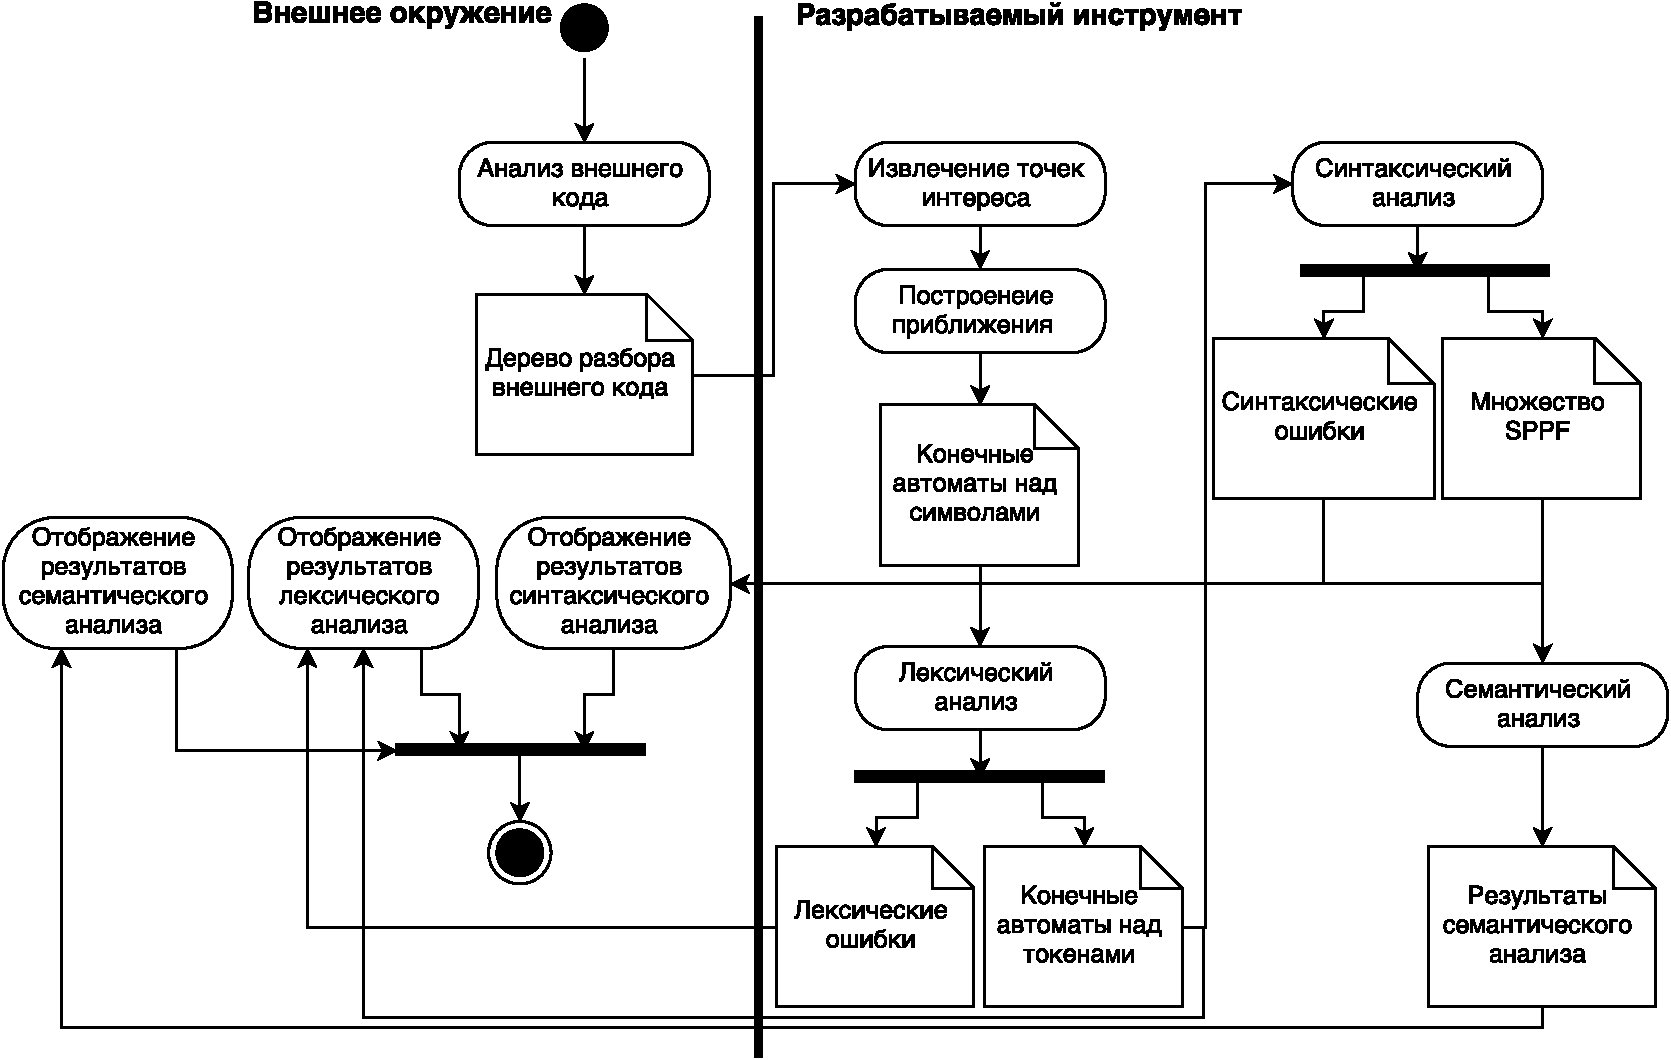
\includegraphics[width=0.9\textwidth]{pics/Activ_SEL_Processing}
\caption{Диаграмма последовательности обработки встроенных языков}
\label{fig:SeqSelProcessing} 
\end{center}
\end{figure}


Существующие инструменты для работы со встроенными языками обычно реализуют поддержку какого-то фиксированного набора языков. При этом поддержка нового языка, как правило, требует нетривиальнй доработки инструмента. Чтобы получить поддержку встроенного языка без изменений в исходном коде базового инструмента, необходимо предоставить соответствующий механизм. 

Для того чтобы упростить процесс создания конечных инструментов, создан SDK, одной из компонент которого является генератор синтаксических анализаторов на основе предложенного в данной работе алгоритма. Также в него входит генератор лексических анализаторов, библиотека построения регулярной аппроксимации, набор вспомогательных функций. Подробное описание компонент приведено далее.

Так как анализ внешнего языка является сложной самостоятельной задачей, то он не включён в разработанный SDK. На вход созданному на основе SDK инструменту должно подаваться дерево разбора внешнего языка с информацией, достаточной для решения поставленных в данной работе задач. 


\subsection{Архитектура YS.SEL.SDK}

Разработанный SDK включает компоненты, необходимые для реализации шагов, представленных на рисунке ~\ref{fig:SeqSelProcessing} и описанных ранее, за исключением анализа внешнего языка. Архитектура SDK изображена на рисунке~\ref{fig:SDKHLArch} и включает в себя генераторы анализаторов и различные библиотеки времени исполнения.

\begin{figure}[h!]
\begin{center}
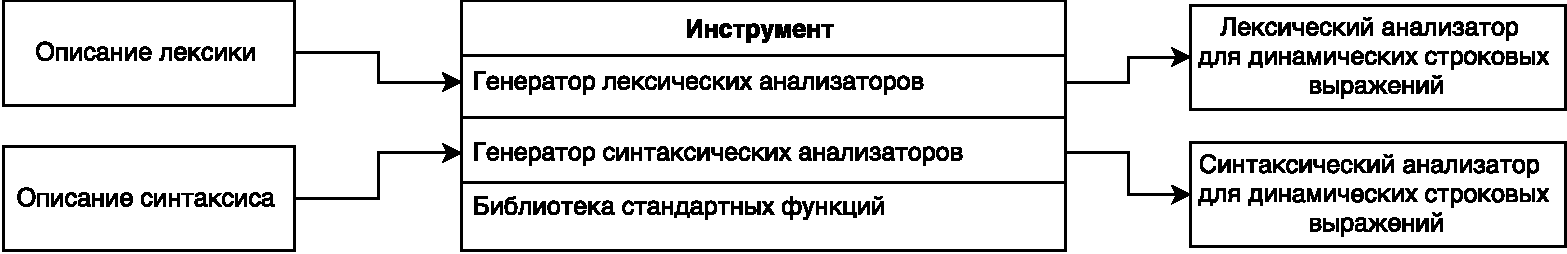
\includegraphics[width=0.9\textwidth]{pics/HighLevelArch}
\caption{Архитектура SDK целиком}
\label{fig:SDKHLArch} 
\end{center}
\end{figure}

Так как анализ внешнего языка не входит в задачи разработанного SDK, то первый шаг, выполнение которого необходимо обеспечить, --- это построение аппроксимации. В нашем случае строится регулярное приближение множества значений динамически формируемого выражения.

Построение регулярной аппроксимации основано на алгоритме, изложенном в работе~\cite{RegOverApprox}, который позволяет строить приближение сверху для множества значений выражений. То есть $L_R$, задаваемый регулярным приближением, не меньше, чем $L_1$, задаваемый программой (выполняется включение $L_R \in L_1$). Это позволяет говорить о надёжности дальнейших анализов в том смысле, что они не теряют информации о $L_1$. Например, это важно при поиске ошибок. Если в $L_R$ не обнаружено ошибок (то есть $L_R \in L_2$, где $L_2$ --- эталонный), значит и в $L_1$ ошибок нет. При этом могут быть найдены ошибки в $L_R$, которых нет в $L_1$, то есть будут ложные срабатывания. Однако наличие ложных срабатываний лучше, чем пропущенные ошибки, и их количество может быть уменьшено путём повышения точности аппроксимации. 

Для того чтобы сделать построение приближения независимым от внешнего языка, реализовано обобщённое представление графа потока управления (Control Flow Graph, CFG)~\cite{Dragon}, которое содержит всю необходимую для дальнейшей работы информацию. Таким образом, разработчику необходимо реализовать построение обобщённого представления CFG для конкретного внешнего языка. В результате компонента строит конечный автомат, являющийся приближением множества значений динамически формируемых выражений.

Архитектура компоненты, отвечающей за лексический анализ, представлена на рисунке~\ref{fig:LexArch}. Основой является  лексический анализатор, который состоит из двух частей: генератора лексических анализаторов, который по описанию лексики обрабатываемого языка, задаваемой в виде файла с расширением fsl (Lexer.fsl), строит соответствующий конечный преобразователь, и интерпретатора, который производит анализ входной структуры данных на основе построенного генератором преобразователя. Конечный преобразователь, построенный по входной спецификации, описывается с виде кода на языке F\# и сохраняется в файле (Lexer.fs). Далее данный файл может быть использован в пользовательском приложении, в рамках которого разрабатывается лексический анализатор, который устроен следующим образом. На вход принимается конечный автомат над символами, результатом работы является конечный автомат над алфавитом токенов анализируемого языка, полученный с помощью интерпретатора и преобразователя, построенного генератором. Входной конечный автомат может быть построен с помощью компоненты построения регулярной аппроксимации. Основные структуры данных --- конечный автомат и конечный преобразователь --- и функции работы с ними описаны в соответствующей библиотеке.

\begin{figure}[h!]
\begin{center}
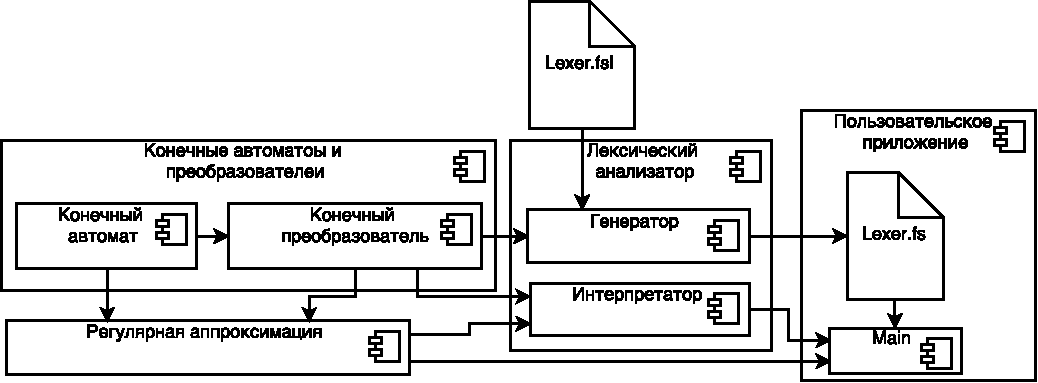
\includegraphics[width=0.95\textwidth]{pics/LexerDiagram}
\caption{Архитектура лексического анализатора}
\label{fig:LexArch} 
\end{center}
\end{figure}

Лексический анализатор реализован на основе инструмента FsLex, который является стандартным генератором лексических анализаторов для языка F\#. При реализации был переиспользован язык описания лексики и некоторые структуры данных.

Реализованный генератор лексических анализаторов обладает следующими особенностями.
\begin{itemize}
    \item Поддерживаются разрывные токены, то есть токены формируемые из нескольких строковых литералов.
    \item Сохраняется привязка лексических единиц к исходному коду: сохраняется информация о строковом литерале, из которого породился токен и координаты его внутри этой строки. Так как одна лексическая единица может формироваться из нескольких строковых литералов, то привязка сохраняется отдельно для каждой части.
    \item Поддерживается обработка входных конечных автоматов, содержащих циклы.
    \item Так как значение токена может формироваться с помощью цикла и, как следствие, быть бесконечным, то каждый токен содержит конечный автомат, порождающий все возможные значения для данного токена, а не единственное значение, как это реализовано в классическом лексическом анализе.
\end{itemize}

\textbf{Генератор синтаксических анализаторов}, названный ARNGLR, реализован на основе алгоритма, описанного в разделе~\ref{AlgoDescr}. Его архитектура представлена на рисунке~\ref{fig:ParsArch}.  

\begin{figure}[h!]
\begin{center}
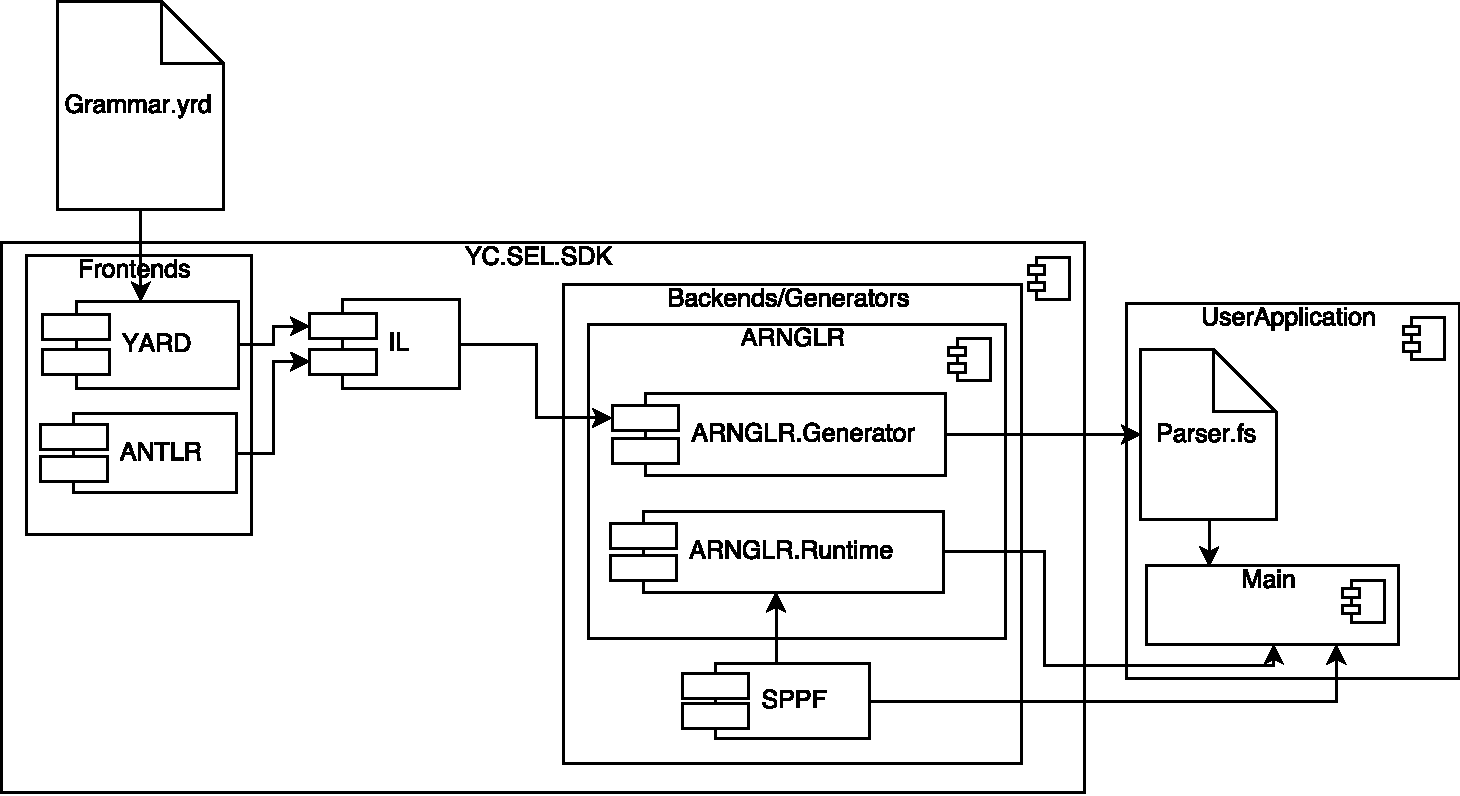
\includegraphics[width=0.95\textwidth]{pics/ARNGLRArch}
\caption{Архитектура синтаксического анализатора}
\label{fig:ParsArch} 
\end{center}
\end{figure}

Генератор реализован как один из модулей YC и может принимать на вход внутреннее представление грамматики (IL), которое может быть получено с помощью различных фронтендов (Frontends), однако в рамках YC.SEL.SDK 
основным фронтендом является YARD, так как он предоставляет наиболее развитые средства для описания грамматик. По грамматике обрабатываемого языка строятся управляющие таблицы анализатора, которые сохраняются в файле Parser.fs. 
Построенные таблицы должны быть включены в разрабатываемое приложение UserApplication. Интерпретатор, предназначенный для синтаксического разбора конечного автомата, полученный после лексического анализа, реализован 
в виде отдельной библиотеки ARNGLR.Runtime, которая также должна быть подключена к разрабатываемому приложению. В результате работы интерпретатора будет получен SPPF, который может быть использован для дальнейшей 
обработки (например, подсчёта метрик). Для упрощения работы с SPPF реализован ряд вспомогательных функций.

\subsection{Архитектура YC.SEL.SDK.ReSharper}

ReSharper --- это расширение к Microsoft Visual Studio IDE, предоставляющее широкий спектр  дополнительной функциональности по анализу и рефакторингу кода. ReSharper поддерживает несколько языков, например C\#, Visual Basic .NET, JavaScript, и этот список может быть расширен благодаря наличию свободно распространяемого ReSharper SDK, описание которого было представлено ранее в разделе~\ref{ReSharperSDKDescr}. ReSharper.SDK позволяет получить деревья разбора для поддерживаемых языков, предоставляет набор готовых анализов и упрощает взаимодействие с Microsoft Visual Studio IDE и её компонентами. Более того, предоставляется возможность разработки собственных расширений для ReSharper на основе ReSharper.SDK.

Microsoft Visual Studio является достаточно распространённой средой разработки, но не поддерживает встроенные языки, поэтому было решено разработать ряд расширений к ReSharper с использованием разработанного инструментария, которые будут устранять данный недостаток. Стоит отметить, что не ставилось задачи поддержать все встроенные языки, так как встроенным может быть любой язык программирования. Также не было необходимости поддержать все внешние языки программирования. Необходимо на базе разработанного YC.SEL.SDK создать инфраструктуру, позволяющую реализовывать поддержку новых встроенных языков в Microsoft Visual Studio через расширения к ReSharper и реализовать несколько расширений, демонстрирующих возможности созданной инфраструктуры. 

Так как необходимо поддерживать различные языки, то необходимо обеспечить расширяемость по новыми языками. Классический подход к решению такой задачи для интегрированных сред разработки заключается в том, что поддержка нового языка реализуется в виде независимой компоненты. Если пользователь хочет получить поддержку какого-либо языка в своей среде разработки, то он должен установить соответствующий пакет. При этом поддержка различных языков осуществляется независимо, однако часто выделяется общая функциональность, которая может быть оформлена в виде отдельного пакета.

Для предоставления описанных выше возможностей была реализована надстройка над YC.SEL.SDK, упрощающая создание расширений для ReSharper, названная  YC.SEL.SDK.ReSharper. В неё включены компоненты, реализующие функции, которые упрощающают взаимодействие YC.SEL.SDK и ReSharper.SDK. Назначени основных из них описаны ниже.

\begin{itemize}
  \item Общая точка расширения, необходимая для подключения функциональности для различных встроенных языков, которая может быть реализована в различных расширениях, к ReSharper через общий интерфейс. Также общая точка расширения позволяет использовать общую функциональность, необходимую для работы со встроенными языками.
  \item Отображение в IDE информации, полученной в ходе анализа. Например, подсветка синтаксиса и ошибок. Вывод диагностических сообщений с информацией об ошибках.
  \item Преобразование данных, из формата, используемого в ReSharper.SDK, в формат для YC.SEL.SDK. Например, преобразование графа потока управления внешнего языка, построенного ReSharper.SDK, в формат, пригодный для построения регулярной аппроксимации средствами YC.SEL.SDK.
  \item Управление работой анализаторов, необходимое, с одной стороны, для обеспечения своевременной реакции на изменения в коде, совершённые пользователем, а с другой, для прекращения вычислений, результаты которых уже не актуальны. Управление построено на основе общего для ReSharper механизма, обеспечивающего асинхронную работу анализов. При этом вычисления могут быть прерваны, если, например, пользователь внёс в код изменения, делающие анализ или его результаты некорректными. 
\end{itemize}

Как уже говорилось, встроенными могут быть различные языки и учесть заранее все их особенности не представляется возможным. Кроме того, даже при использовании одного встроенного языка могут использоваться различные способы выполнения сформированного запроса. Таким образом, необходимо предоставлять возможность настройки расширений конечным пользователем. Для этого в рамках YC.SEL.SDK.ReSharper была реализована возможность управления следующими основными параметрами расширений. 

\begin{itemize}
    \item Подсветка синтаксиса для каждого языка. Предоставлена возможность указать цвет для каждого типа токена.
    \item Указание парных элементов. Для каждого языка можно указать, какие лексические единицы считать парными: для каждой пары указывается ``левый'' (открывающая скобка) и ``правый'' (закрывающая скобка) элементы. При расположении курсора в тексте рядом с одним из элементов пары будут подсвечены соответствующие элементы. Пример подсветки парных элементов приведён на рисунке~\ref{fig:braces}.
    \item Точки интереса или хотспоты (hotspot) --- это места, в которых должно быть сформировано финальное выражение. Необходимо знать, какой хотспот какому языку соответствует. При этом нужно учитывать, что одному языку может соответствовать несколько хотспотов. Например, динамически сформированный SQL-запрос в программе на языке программирования C\# может быть выполнен с помощью метода \verb|ExecuteQuery| класса \verb|DataContext|~\cite{ExecuteQuery}
     или же текст запроса может быть передан как аргумент конструктора класса \verb|SqlCommand|~\cite{SqlCommand} с последующим выполнением с помощью метода \verb|ExecuteReader|.

\end{itemize}

Настройка указанных выше параметров хранится в соответствующих конфигурационных файлах в формате XML, которые на данный момент редактируются вручную. Настройка подсветки синтаксиса и парных элементов совмещена в одном файле и для каждого языка создаётся отдельный такой файл. Конфигурационный файл с точками интереса является общим для всех языков и, соответственно, для всех установленных расширений для поддержки встроенных языков.

В листинге~\ref{lst:codeHighlighting} приведён пример конфигурации подсветки синтаксиса и парных скобок для языка Calc. Для указания цвета используются имена, принятые в ReSharper (например, \verb|"CONSTANT_IDENTIFIER_ATTRIBUTE"|), что должно сделать настройку цветов более единообразной. В xml-тэге \verb|Matched| содержится описание парных элементов. Каждая пара описывается в xml-тэге \verb|Pair| и для одного языка может быть указано более одной такой пары.

\fvset{frame=lines,framesep=5pt}
\begin{listing}[H]
    \begin{pyglist}[language=xml,numbers=left,numbersep=5pt]
<?xml version="1.0" encoding="utf-8"?>
<SyntaxDefinition name="CalcHighlighting">
    <Colors>
        <Tokens color="CONSTANT_IDENTIFIER_ATTRIBUTE">
            <Token> DIV </Token>
            <Token> LBRACE </Token>
            <Token> MINUS </Token>
            <Token> MULT </Token>
            <Token> NUMBER </Token>
            <Token> PLUS </Token>
            <Token> POW </Token>
            <Token> RBRACE </Token>
        </Tokens>
    </Colors>
<!-- Dynamic highlighting: -->
    <Matched>
        <Pair>
            <Left> LBRACE </Left>
            <Right> RBRACE </Right>
        </Pair>
<!-- You can specify more then one pair:        
        <Pair>
            <Left> LEFT_SQUARE_BRACKET </Left>
            <Right> RIGHT_SQUARE_BRACKET </Right>
        </Pair>
        <Pair>
            <Left> LEFT_FIGURE_BRACKET </Left>
            <Right> LEFT_FIGURE_BRACKET </Right>
        </Pair>
-->        
    </Matched>
</SyntaxDefinition>
    \end{pyglist}
\caption{Пример конфигурационного файла для настройки подсветки синтаксиса}
\label{lst:codeHighlighting}
\end{listing}

Листинг~\ref{lst:hotspots} содержит пример описания точек интереса. Для каждой точки интереса должна быть указана следующая информация.
\begin{itemize}
    \item Какому встроенному языку соответствует точка. Информация хранится в Xml-тэге \verb|Language|.
    \item Полное имя метода, являющегося точкой интереса. Информация хранится в Xml-тэге \verb|Method|.
    \item Порядковый номер аргумента данного метода, являющегося выражением на встроенном языке. Нумерация начинается с нуля. Информация хранится в Xml-тэге \verb|ArgumentPosition|. 
    \item Возвращаемый тип метода.  Информация хранится в Xml-тэге \verb|ReturnType|. 
\end{itemize}

\fvset{frame=lines,framesep=5pt}
\begin{listing}[H]
    \begin{pyglist}[language=xml,numbers=left,numbersep=5pt]
<?xml version="1.0" encoding="utf-8"?>
<!-- comment about body -->
<Body>
    <!-- comment about hotspot -->
  <Hotspot>
      <!-- comment about tsql -->
      <Language> TSQL </Language>
      <!-- comment about fullName -->
      <Method>Program.ExecuteImmediate</Method>
      <!-- zero-based -->
      <ArgumentPosition> 0 </ArgumentPosition>
      <!-- comment about return type -->
      <ReturnType> void </ReturnType>
  </Hotspot>
  <Hotspot>
      <Language> Calc </Language>
      <Method>Program.Eval</Method>
      <ArgumentPosition> 0 </ArgumentPosition>
      <ReturnType> int </ReturnType>
  </Hotspot>
</Body>
    \end{pyglist}
\caption{Пример конфигурационного файла для настройки точек интереса}
\label{lst:hotspots}
\end{listing}


\section{Области и способы применения YC.SEL.SDK}

Разработанный SDK предназначен для создания инструментов статического анализа динамически формируемых строковых выражений. Решения, созданные с его помощью, могут применяться для работы с проектами, активно использующими динамически формируемые строковые выражения. Необходимость работать с такими проектами может возникнуть, например, в следующих областях.

\begin{itemize}
    \item Реинжиниринг программного обеспечения.
    \item Поддержка встроенных языков в средах разработки.
    \item Оценка качества и сложности кода.
\end{itemize}

Общим для всех этих областей является то, что для решения многих задач необходимо структурное представление динамически формируемого кода. При этом анализируемые языки могут быть различными и процесс их анализа часто тесно связан с анализом внешнего языка.

Отметим, что встроенные языки используются всё менее активно в молодых проектах и системах. На смену им приходят более надёжные способы композиции языков и метапрограммирования. Например LINQ или ORM-технологии. Однако это не всегда так. Использование строковых выражений для взаимодействия с базами данных и генерации WEB-страниц в приложениях на PHP всё ещё широко распространено~\cite{DSQLInActiveUse}. Это необходимо учитывать при поддержке встроенных языков в средах разработки. Для каких-то языков на первый план выходят возможности по изучению и модификации уже созданного кода, а для каких-то --- возможность быстро и удобно создавать новый код. Во втором случае могут возникнуть дополнительные требования к скорости работы инструмента, так как подразумевается выполнение некоторых операций ``на лету'', что может послужить ограничением на использование SDK, так как многие механизмы, реализованные в нём, не предусматривают возможности уменьшения точности в пользу увеличения быстродействия. Оценка качества и сложности  кода часто может выполняться в рамках комплекса задач по реинжинирингу системы, однако может быть и самостоятельной задачей, например, при оценке сложности работ по поддержке и сопровождению информационной системы.

Детали применения SDK могут варьироваться в зависимости от решаемых задач и контекста использования. Например, механизм построения регулярной аппроксимации может быть реализован независимо в рамках внешнего инструмента. Однако основной сценарий использования аналогичен использованию инструментариев для разработки компиляторов. Последовательность шагов, представленная ниже, может быть изменена в зависимости от особенностей задачи.

\textbf{Шаг 1.} Создание грамматики обрабатываемого языка. Грамматика может быть создана на основе документации соответствующего языка или переиспользована готовая, что оправданно, например, при создании анализатора для динамического SQL, когда внешний и встроенный языки совпадают.

\textbf{Шаг 2.} Генерация синтаксического анализатора по созданной грамматике. Для этого используется генератор синтаксических анализаторов, присутствующий в SDK. Результатом работы генератора является файл с исходным кодом на языке программирования F\#, который должен быть включён в разрабатываемый код. Файл содержит описание типов для лексических единиц, управляющие таблицы анализатора и функцию, которая по конечному автомату над алфавитом токенов анализируемого языка построит SPPF, содержащий деревья вывода всех корректных цепочек.

\textbf{Шаг 3.} Создание лексической спецификации обрабатываемого языка. Спецификация может быть извлечена из документации или заимствована из других проектов. При обработке динамически формируемого SQL возможно переиспользовать спецификацию, созданную для основного языка, которым также является SQL. При этом необходимо обратить внимание на то, что типы лексических единиц определяются на основе созданного на предыдущих шагах синтаксического анализатора.

\textbf{Шаг 4.} Генерация лексера по созданной спецификации. Для этого применяется генератор лексических анализаторов, входящий в состав SDK. В результате его применения получается файл с исходным кодом на языке F\#, который должен быть подключён к разрабатываемому решению. 

\textbf{Шаг 5.} Реализация механизма построения регулярной аппроксимации, результатом которого является функция, строящая конечный автомат над алфавитом символов. Данный механизм может быть реализован либо на основе предоставляемого в рамках SDK, либо независимо. В первом случае от разработчика требуется построить обобщённый CFG для внешнего языка. Во втором случае необходимо только гарантировать правильность возвращаемого конечного автомата. Второй подход может быть использован, например, при наличии реализованного механизма протягивания констант для внешнего языка. Это позволит создать возможно менее точное, но, скорее всего, более быстрое построение аппроксимации. Такой подход применим при автоматизированном реинжиниринге, когда ручная доработка кода является обязательным шагом и абсолютная точность автоматической обработки не требуется. Ещё одна возможная область применения второго подхода --- это поддержка встроенных языков в средах разработки. Здесь также часто не требуется высокая точность для подсказок пользователю, однако производительность крайне важна. Поэтому иногда приходится жертвовать точностью анализа для достижения нужной скорости работы.

\textbf{Шаг 6.} Реализация работы с SPPF. Синтаксический анализатор возвращает SPPF --- конечное представление леса разбора всех корректных цепочек из аппроксимации. Дальнейшая работа с ним может строиться по двум основным сценариям.

Превый сценарий --- непосредственная обработка SPPF. В этом случае все вычисления происходят над SPPF без извлечения отдельных деревьев. Это позволит ускорить обработку результатов разбора, так как количество деревьев может быть бесконечным, а SPPF является конечной структурой данных. Однако существует несколько проблем, связанных с таким подходом. Во-первых, требуется создание новых процедур обработки, так как классические, как правило, ориентированы на работу с деревьями. Во-вторых, могут возникнуть трудности при выполнении некоторых анализов, вызванные тем, что в SPPF хранятся ``бесконечные'' деревья. Например, необходимо вычислить максимальную глубину вложенности конструкции \verb|if|, являющуюся одной из стандартных метрик сложности кода. SPPF может содержать 
циклы и может оказаться так, что конструкция \verb|if| встречается в цикле таким образом, что потенциальная глубина вложенности может быть бесконечной. Такая ситуация не является стандартной при 
обработке деревьев разбора и её надо отслеживать отдельно.

Второй сценарий --- извлечение отдельных деревьев из SPPF и их обработка. Данный подход может оказаться удобным, если уже существуют процедуры обработки синтаксических деревьев для языка, который оказался встроенным. Это помогает избежать затрат на создание новой функциональности. Такое может произойти при работе с динамическим SQL. В этом случае для работы с деревом разбора внешнего языка и деревьями, извлечёнными из SPPF, можно использовать одни и те же процедуры, так как языки идентичны.

Недостатком второго подхода является то, что конечность числа деревьев не гарантирована. Это значит, что не удастся обработать все деревья. Стоит отметить, что даже в случае конечности числа деревьев, перебор и обработка всех деревьев разбора может потребовать значительных ресурсов.


\textbf{Шаг 7.} Реализация механизмов сбора, обработки и отображения информации, такой как сообщения об ошибках или любой другой, полученной в процессе анализа. Необходимо для предоставления пользователю информации, ожидаемой в рамках решаемой задачи.

На рисунке~\ref{fig:activMethod} изображён один из возможных сценариев использования SDK. Особенностью является цикличность процесса, характерная, например для реинжиниринга программного обеспечения.

\begin{figure}[h!]
\begin{center}
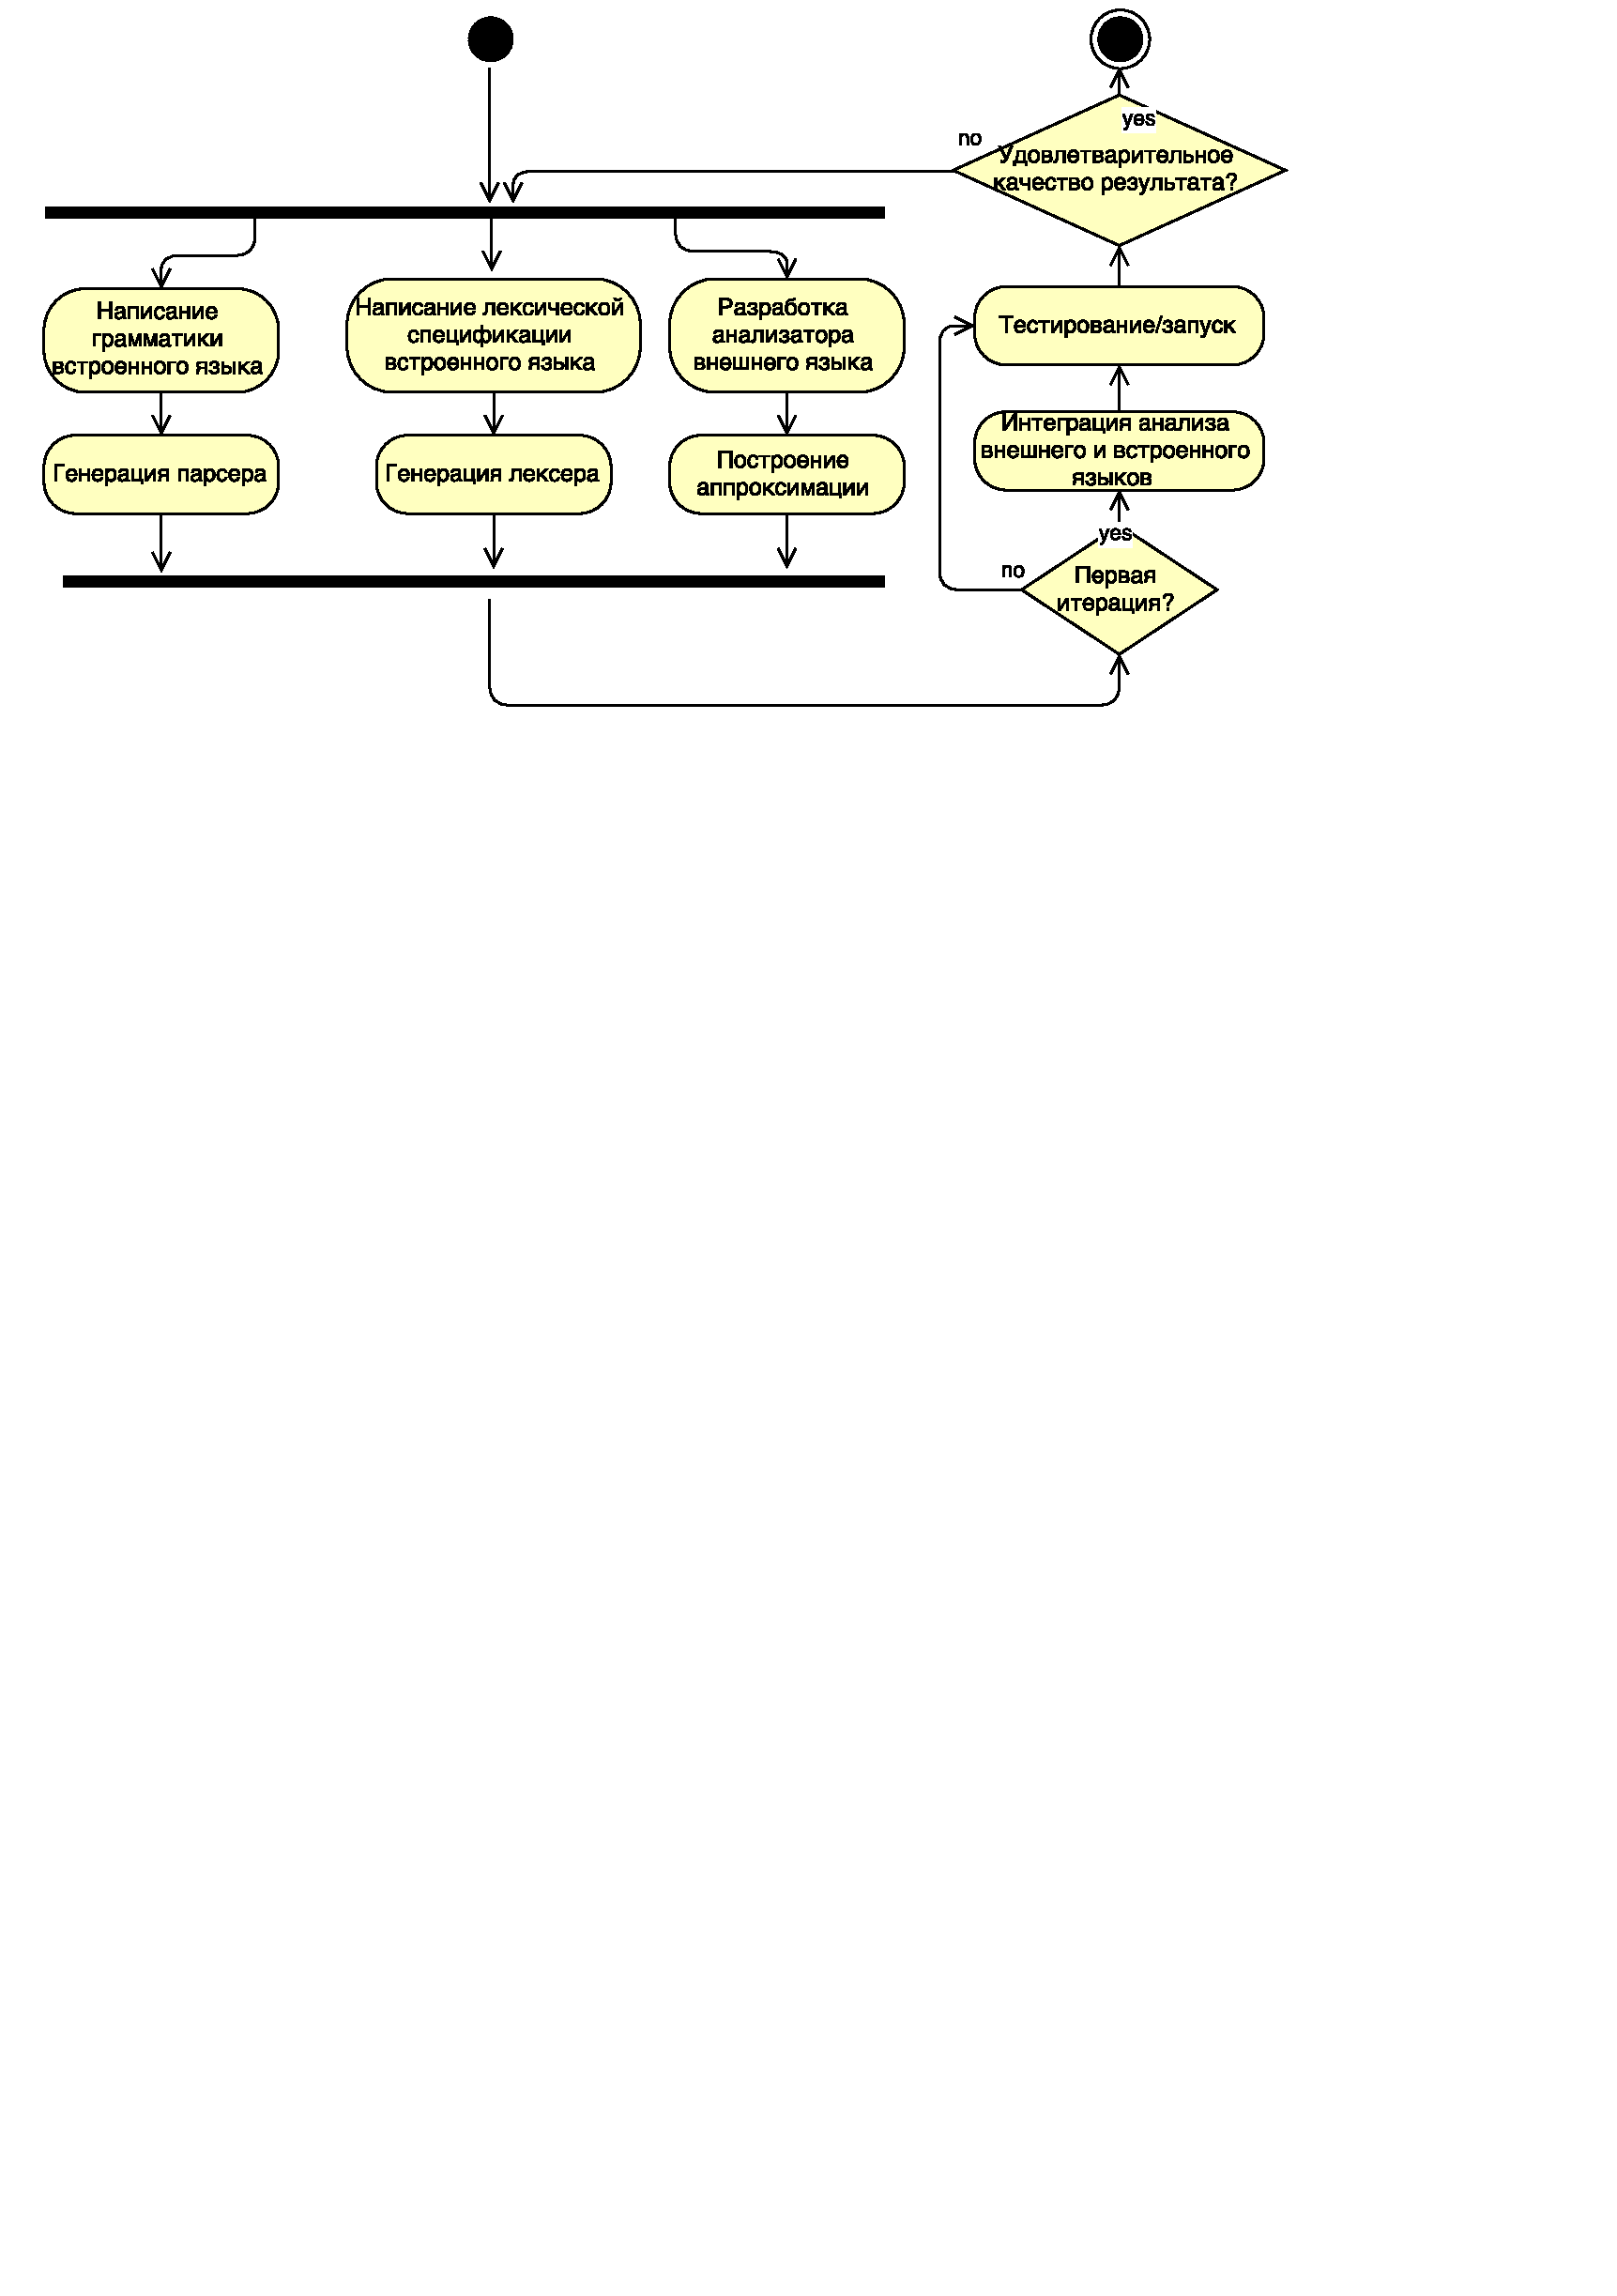
\includegraphics[width=0.9\textwidth]{pics/ActivMethodology}
\caption{Один из возможных вариантов использования SDK в проектах по реинжинирингу}
\label{fig:activMethod} 
\end{center}
\end{figure}

Встраивание анализа строковых выражений в последовательность обработки кода всей системы зависит от решаемых задач. Первыми шагами идут действия, необходимые для того, чтобы получить входные данные для анализа. Для этого необходимо провести лексический и синтаксический анализ внешнего языка, построить граф потока управления. После этого возможно построение аппроксимации и дальнейший анализ встроенных языков. Параллельно с этим может проводиться дальнейшая обработка внешнего языка. Степень параллельности зависит от независимости решаемых задач. Например, некоторые метрики сложности для основного кода и для динамически формируемого можно считать независимо и выводить отдельно. С другой стороны, может возникнуть необходимость вычислить некую комплексную метрику, учитывающую параметры и внешнего и динамически формируемого кода, что приведёт к необходимости синхронизации.

\section{Особенности реализации}

Разработка инструментального пакета с описанной выше архитектурой и плагинов для ReSharper велась в рамках исследовательского проекта YaccConstructor (YC), описанного в разделе~\ref{YCDescr}. 
Разработка велась на платформе .NET и основной язык реализации --- F\#~\cite{FSharp}. Весь исходный код опубликован на GitHub~\cite{YCUrl}. 
Большинство компонент опубликовано под ``открытой'' лицензией Apache License Version~2.0~\cite{ApacheV2}. 

За основу алгоритма синтаксического анализа динамически формируемых выражений был взят реализованный в YC алгоритм синтаксического анализа RNGLR. Генератор управляющих таблиц был использован практически без 
модификаций, а интерпретатор был реализован отдельный. Кроме этого, общими являются некоторые структуры данных и вспомогательные функции, такие как представление леса разбора и его печать в формате 
DOT~\footnote{DOT --- текстовый язык описания графов~\cite{DOT}.}, представление GSS. 

Лексичекий анализ реализован на основе инструмента FsLex, который потребовал значительных доработок для того, чтобы обеспечить обработку конечного автомата, а не линейного входа. Все остальные компоненты, 
необходимые для статического анализа динамически формируемых выражений, такие как построение аппроксимации, вспомогательные функции для упрощения построения целевых инструментов были реализованы ``с нуля'' 
в рамках проекта YC.

Бинарные пакеты, содержащие основную функциональность, опубликованы в сети интернет на NuGet~\footnote{NuGet --- менеджер пакетов для платформы .NET и одноимённый ресурс для их публикации. Позволяет публиковать 
и устанавливать пакеты, автоматически отслеживать зависимости между ними~\cite{NuGet}.}.

\chapter{Метод реинжиниринга информационных систем, использующих дмнамически формируемые выражения}

В данной главе изложен метод проведения реинжинирига информационных систем, использующих строковые встроенные языки (string-embedded languages~\cite{Alvor1}). Рассмотрены основные типы задач, решаемых при реинжиниринге, указаны особенности обработки встроенных языков при их решении. Основной акцент сделан на обработку динамически формируемого SQL-кода, однако изложенный метод может быть адаптирован к обработке систем, использующих другие встроенные языки.

\section{Особенности}

Реинжиниринг информационных систем как правило является комплексным мероприятием, которое может в ключать в себя различные шаги, такие как анализ кода и его изучение, его рефактоинг, трансформацию, перенос на другие программно-аппаратные платформы~\cite{reengANT}. При этом часто проводится комплексный анализ многокомпонентной системы целиком, что приводит к необходимости уитывать различные особенности системы и работать с разнородными артефактами: документацией, исходным кодом, конфигурационными скриптами, скриптами баз данных и т.д. Всвязи с высокой сложностью такого анализа, ренжиниринг, как правило, является автоматизированным, а не полностью автоматическим процесс, что означает возможность (и необходимость) активного участия человека. Это позволяет использовать инструменты, которые не приводят сразу к получению конечнго результата, однако минимизируют ресурсы, необходимые для решения задачи. Например, может оказаться, что в системе присутствуют файлы особого формата и для их автоматической обработки потребуется создание уникального инструмента, что потребует значительных ресурсов. Однако объём этих файлов мал и их ручной анализ прост. В ситуации, когда затраты на создание инструмента значительно выше затрат на ручной анализ с тем же качеством результата, часто оказывается выгоднее отказаться от создания инструмента.

С одной стороны, динамически формируемый код может содержать важную информацию о системе. Например, в динамически формируемых SQL-запросах могут содержаться сведения о схеме данных и особенностями работы с базой данных, не извлекаемые из внешнего кода. С другой стороны, при активном использовании динамически формируемый код является сущьностью, требующей отдельного внимания при обработке системы и, следовательно, должен быть учтён, например, при оценки сложности системы, часто проводимой на начальных этапах при определении сроков и стоимости работ.

Системы используют строковые встроенные языки с разной интенсивностью и разными способами. В зависимости от характера использования встроенных языков меняются требования к автоматизации их обработки: необходима ли инструментальная поддержка или ручная обработка потребует меньше ресурсов, чем создание или освоение инструмента, какими именно инструментами пользоваться в тех или иных случаях.

Метода не обнаружено. Надо предложить свой.


\section{Метод}

Как было сказано ранее, встроенным языком может оказаться любой язык, однако на практике достаточно широко распространено использование днамически формируемого SQL-кода и генерация HTML-страниц. Использование динамически формируемого кода на других языках встречается реже. По этим причинам далее описан метод реинжиниринга систем, использующих встроенный SQL, однако он может быть адаптирован и к обработке систем, использующих другие встроенные языки. Схема метода представлена на рисунке~\ref{fig:method}, а детальное описание шагов приведено далее.

\begin{figure}[h!]
\begin{center}
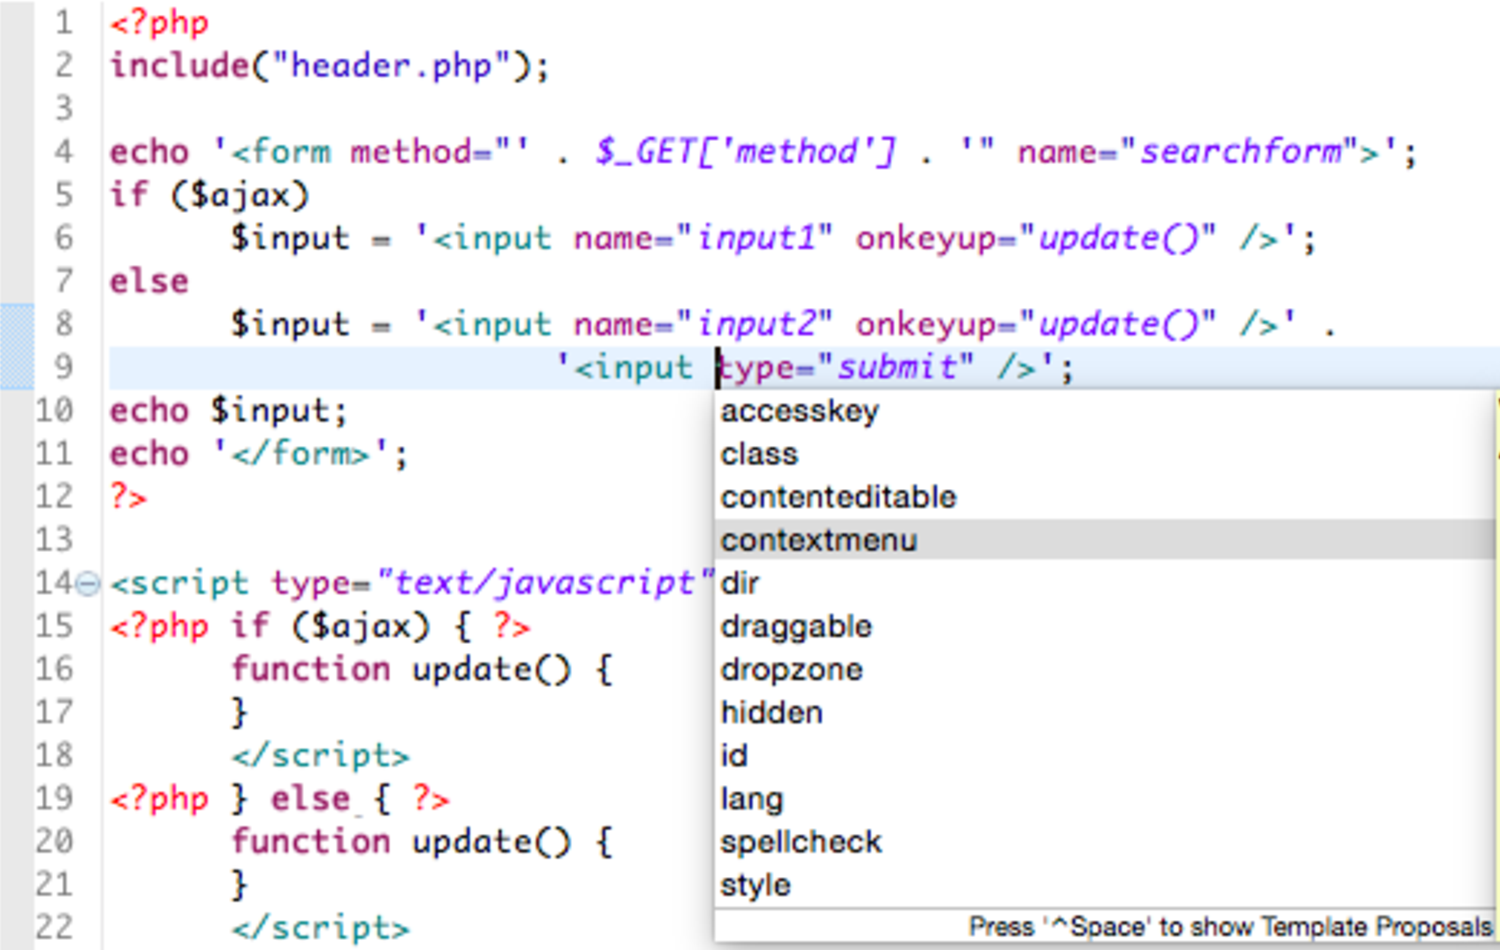
\includegraphics[width=.9\textwidth]{pics/Varis.pdf}
\caption{Пример функциональности Varis: автодополнение и подсветка синтаксиса во встроенном HTML в среде разработки Eclipse}
\label{fig:method} 
\end{center}
\end{figure}


%\begin{longtable} [htbp]
{\small
  \centering
  
  \begin{longtable}{| r | p{2cm} | p{4cm} | p{2cm} | p{7cm} |}
  
  \hline                               
  \hline
  \textnumero & Что & Зачем & Вход & Ответ \\
  \hline 
  \multirow{2}{*}1 
  &
  \multirow{2}{*}{\begin{minipage}{2cm}Анализ целей и задач\end{minipage}}
  &
  Что нужно сделать
  & 
  Задачи
  &
  Список задач, при решении которых необходимо обрабатывать динамически формируемый код
  \\  
  & 
  &
  Зачем
  &
  Цели
  &
  Планиоуется ли модицикафия и сопровождение
  \\
  \hline
  \multicolumn{5}{|p{16cm}|}{Дальнейшие шаги выполняются, если список задач, требующих обработку встроенного кода не пуст.}\\
  \hline
  \multirow{2}{*}2 
  &
  \multirow{2}{*}{\begin{minipage}{2cm}Первичный анализ системы\end{minipage}}
  &
  Сколько в системе встроенного кода
  & 
  Код
  &
  Количество точек выполнения 
  \\  
  & 
  &
  На сколько сложно формируется код
  &
  Код
  &
  Для каждой точки выполнения количество операторов, участвующих в формировании соответствующего запроса.
  \\
  \hline
 
  \multirow{3}{*}3 
  &
  \multirow{3}{*}{\begin{minipage}{2cm}Доступ к сиситеме\end{minipage}}
  &
  Важность наличия доступа
  & 
  Список задач
  &
  Есть ли задачи, отражаюиеся на рантайме
  \\  
  & 
  &
  Доступ на чтение
  &
  Заказчик
  &
  Для каждой точки выполнения количество операторов, участвующих в формировании соответствующего запроса.
  \\
  & 
  &
  Возможность изменять
  &
  Заказчик
  &
  Для каждой точки выполнения количество операторов, участвующих в формировании соответствующего запроса.
  \\
  \hline
 
  \multirow{3}{*}4 
  &
  \multirow{3}{*}{\begin{minipage}{2cm}Роль дфк\end{minipage}}
  &
  А надо ли
  & 
  Список задач
  &
  Есть ли задачи, отражаюиеся на рантайме
  \\  
  & 
  &
  для чего
  &
  Код, документация, заказчик
  &
  Для каждой точки выполнения количество операторов, участвующих в формировании соответствующего запроса.
  \\
  & 
  &
  На сколько активно
  &
  Код, документация, заказчик
  &
  Для каждой точки выполнения количество операторов, участвующих в формировании соответствующего запроса.
  \\
  \hline
 
  \multirow{4}{*}5 
  &
  \multirow{4}{*}{\begin{minipage}{2cm}Анализ ресурсов\end{minipage}}
  &
  А надо ли
  & 
  Список задач
  &
  Есть ли задачи, отражаюиеся на рантайме
  \\  
  & 
  &
  На сколько критичен дфк
  &
  роль дфк
  &
  Для каждой точки выполнения количество операторов, участвующих в формировании соответствующего запроса.
  \\
  & 
  &
  Как можем оценить
  &
  доступ к системе
  &
  Для каждой точки выполнения количество операторов, участвующих в формировании соответствующего запроса.
  \\
  & 
  &
  Есть ли запас
  &
  Заказчик
  &
  Для каждой точки выполнения количество операторов, участвующих в формировании соответствующего запроса.
  \\
  \hline
 
  \multirow{3}{*}6 
  &
  \multirow{3}{*}{\begin{minipage}{2cm}Особенности\end{minipage}}
  &
  Зачем
  & 
  список задач
  &
  Надо знать, на какие особенности обращать внимание.
  \\  
  & 
  &
  Существуют ли впринципе
  &
  Список задач, знания языков
  &
  Список особенностей
  \\
  & 
  &
  Есть ли в системе
  &
  код
  &
  Список особенностей
  \\
  \hline
 
  \multirow{6}{*}7 
  &
  \multirow{6}{*}{\begin{minipage}{2cm}Подход\end{minipage}}
  &
  Сопровождение результатов
  & 
  цели
  &
  Есть ли задачи, отражаюиеся на рантайме
  \\  
  & 
  &
  Доступ к системе
  &
  доступ к системе
  &
  Для каждой точки выполнения количество операторов, участвующих в формировании соответствующего запроса.
  \\
  & 
  &
  Доступность ресурсов
  &
  анализ ресурсов
  &
  Для каждой точки выполнения количество операторов, участвующих в формировании соответствующего запроса.
  \\
  & 
  &
  Точность
  &
  Задачи
  &
  Для каждой точки выполнения количество операторов, участвующих в формировании соответствующего запроса.
  \\
  & 
  &
  Особености
  &
  Особенности
  &
  Есть ли особенности, влияющие на выбор подхода.
  \\
  & 
  &
  Задачи
  &
  Срисок задач
  &
  Для каждой точки выполнения количество операторов, участвующих в формировании соответствующего запроса.
  \\
  \hline
 
  \multirow{4}{*}8 
  &
  \multirow{4}{*}{\begin{minipage}{2cm}Выбор решения\end{minipage}}
  &
  Требуется ли внутреннее представление
  & 
  Задачи
  &
  Есть ли задачи, отражаюиеся на рантайме
  \\  
  & 
  &
  Сложные случаи
  &
  Особенности
  &
  Для каждой точки выполнения количество операторов, участвующих в формировании соответствующего запроса.
  \\
  & 
  &
  Динамика, статика
  &
  подход
  &
  Для каждой точки выполнения количество операторов, участвующих в формировании соответствующего запроса.
  \\
  & 
  &
  Точность
  &
  Заказчик
  &
  Для каждой точки выполнения количество операторов, участвующих в формировании соответствующего запроса.
  \\

  
  \hline
  \hline
  \caption{Распределение динамически формируемых SQL-запросов по времени обработки}\label{tbl:method}
  \end{longtable}
%\end{longtable}
}


\begin{enumerate}
  \item \textbf{Анализ целей и задач.}
  
  Проанализировать цели и задачи. От того, какие задачи необходимо решать, напрямую зависит выбор средств и инструментов. Основные классы задач затрагивающих динамически формируемый код, которые можно выделить на данном этапе, приведены ниже.
  
  \begin{itemize}
    \item Оценка качества кода и его сложности, что часто сводится к подсчёту некоторых формальных метрик кода~\cite{SoftwareMetrics, DSQLQualityMesureBIG}. Необходимо определить, требуется ли построение структурного представления кода для вычисления требуемых метрик с необходимой точностью.
    \item Анализ надёжности системы, поиск различного рода уязвимостей и ошибок. Требуется изучение типов ошибок, которые предполагается обнаруживать: обнаружене некоторых типов ошибок требуют построения структурного представления кода (семантические ошибки), вто время, как для других это не требуется (лексические, синтаксические ошибки).
    \item Извлечение или восстановлени утраченных знаний о системе и её изучение.
    \item Трансформация исходной системы: рефакторинг, перенос на новые программно-аппаратные системы.
  \end{itemize}
  
  При этом необходимо проанализировать конечные цели реинжиниринга. Особенно важен данный шаг при необходимости решать задачи трансформации динамически формируемого кода. Например, если целью является как можно более быстрое получение работающей системы, дальнейшее развитие которой не планируется, то можно пожертвовать качаством кода результирующей системы, что может существенно упростить её обработку. Однако, если после выполнения трансформаций планируется активная разработка или поддержка полученной системы, то необходимо получить результирующий код как можно более привычный для разработчиков системы. Это упростит дальнейшую работу с ним, позволит уменьшить затраты на обучение крманды, поиск новых специалистов.
  
  Например, при трансляции хранимого SQL-кода, активно использующего динамический SQL, с одного языка на другой, важно сохранить однородность. Особенно если планируется дальнейшее развитие системы. Это обусловлено тем, что различные диалекты SQL содержат большое количество особенностей и разработчики на SQL часто оказываются специалистами достаточно узкого профиля. Таким образом, наличие двух различных диалектов в место одного, может усложнить набор команды. Более того, в процессе разработки необходимость переключаться между несколькими диалектами так же может вызвать трудности.
  
  Таким образом, необходимо ответить на следующий вопрос: планируется ли активное изменение системы после её реинжиниринга, если он включает трансформации.
  
  \item \textbf{Первичный анализ проекта.} На данном этапе необходимо проанализировать исходный код системы и выяснить характеристики встроенного текстового кода. Для этого, как правило, можно использовать стандартные средства анализа программного кода. Однако, скорее всего они будут требовь модификации, по этому необходимо иметь доступ к исходному коду. Необходимо оценить следующие характеристики.
  \begin{itemize}
    \item Клоичество точек выполнения встроенного кода. Как правило, за выполнение выражений на встроенном языке отвечают характрные языковые конструкции, например \verb|EXECUTE|\footnote{Конструкция язука T-SQL, позволяющая выполнить динамически формируемый звпрос. Документация: \url{https://msdn.microsoft.com/en-us/library/ms188332.aspx}. Посешён 29.07.2015.} в языке T-SQL. следовательно, необходимо оценить количество таких конструкций. Для грубой оценки можно использовать простой текстовый поиск (если такой поиск говорит о полном отсутствии конструкций, то дальнейший анализ можно не проводить). Для более точной оценки необходимо использовать структурное представление кода, чтобы, например, не учитывать код, находящийся в комментариях. Получить структурное представление и доступ к нему можно с помощью библиотек синтаксического анализа соответствующего языка.
    
    \item Сложность формирования строковых выражений. Прежде всего необходимо определить наличие динамически формируемого кода и оценить сложность его формирования, так как в случае использования только константных строковых литеалов не потребуется специальных инструментов для анализа встроенного кода.
    
    Для данной оценки можно использовать протягивания констант. Его необходимо модифицировать таким образом, чтобы он отдельно обрабатывал выражения, отвечающие за формирование кода, и собирал о них следующую информацию о процессе формрования кода как для каждой точки выполнения, так и для всей системы вцелом.
    \begin{itemize}
      \item Количество конкатенаций.
      \item Количество операторов ветвления: \verb|if-then-else|, \verb|switсh-case| и т.д.
      \item Количество строковых функций: \verb|replace|, \verb|substring| и т.д.
      \item Количество циклов, как ``явных'' (\verb|while|, \verb|for|), так и организованных с помощью рекурсии.
      \item Количество переменных, значение для которых нельзя полностью вычислить статически (например, они получают значение из пользовательского входа).
      \item Факт формирования кода в телах более чем одного метода/процедуры. Необходимость межпроцедурного анализа.
    \end{itemize}
  \end{itemize}
  
  \item \textbf{Роль динамически формируемого кода в системе.} На данном шаге необходимо определить, какую роль в функционировании системы играют динамически формируемые запросы. Возможны следующие существенно различные ситуации.
  \begin{itemize}
    \item Использование динамически формируемого кода является один из основных элементов дизайна системы. Данная ситуация, как правило, выделяется большим количеством точек исполнения и наличием сложно формируемого кода. Важно определить, каие именно компонениты системы построены таким образом, так как использование встроенных языков может быть весьма неоднородным. Средние значения по всей системе могут быть не велики, при этом ряд ключевых компонент построены с активным использованием динамически формируемого кода, а в остальных он отсутствует. При этом может оказаться, что ключевые компоненты являются ещё и самыми критическими по производительности учестками системы.
    
    \item Динамически формируемый код используется как вспомогательное средство. Чаще всего явным признаком такой ситуации является его малое количество или полное отсутствие. Однако, это не всегда так. Возможна ситуация, когда динамически формируемых код достаточно активно используется для реализации служебной и вспомогательной функциональности. Тот факт, что данная функциональность не является основной для системы, может позволить обращать меньше внимания, например, на производительность результатов трансформации соответствующего кода.
  \end{itemize}
  
  \item \textbf{Возможности доступа к исходной системе в реальных условиях.} Возможность изучения системы в реальных условиях может дать большое количество полезной информации, которую трудно или дажен невозможно получить другими способами, так как даже тесты часто не воспроизводят реальное функционирование системы. Однако он часто оказывается невозможным или крайне затруднённым, что вызывается, с одной стороны вопросами безопасности, с другой стороны надёжностью, так как гарантировать, что внесённые изменения не отразатся на работоспособности системы часто затруднительно.  
  \begin{itemize}
    \item Есть ли доступ к системе, работающей в реальных условиях? Чтение определённых журнальных файлов, перехват сообщений на каком-либо уровне, доступ к реальной базе данных.
    \item Возможен ли запуск модифицированной системы в реальных условиях? Если мы можем запустить модифицированную систему, то важно убедиться, что будет возможность получить обратно собранную информацию.
    \item Модификации какого рода разрешены? Что можно собирать, а что нельзя.
  \end{itemize}
  
  \item \textbf{Анализ требований к производительности и потреблению ресурсов.} Необходимо определить, можем ли мы позволить себе дополнительные накладные расходы. Ответ на данный вопрос особенно важен при выборе между статическим и динамическим подходом к трансляции динамически формируемого кода. Выполнение динамически формируемых SQL-запросов само по себе требует дополнительных ресурсов. Если на предыдущих шагах было выяснено, что динамически формируемый код активно используется в критическом по произволительности месте, а вычислительные ресурсы ограничены, то применение динамичекого подхода, требующего дополнительных вычислений во время выполнения, может существенно ухудшить быстродействие системы.
  
  \item \textbf{Анализ особенностей конкретного вншнего и встроенного языков.} Многие задачи требуют комплексной обработки внешнего и встроенного кода. Например, при статическом поиске ошибок, включающем ошибки использования типов переменных, необходимо проводить анализ, проверяющий, что тип переменной во внешнем коде соответствует типу, возвращаемому запросом. Пример несовпадения типов приведён в листинге~\ref{lst:typeChecking}: : переменная \texttt{result} имеет тип \texttt{List<string>}, однако запрос возвращает коллекцию двухэлементных кортежей.
  
\fvset{frame=lines,framesep=5pt}
\begin{listing}
    \begin{pyglist}[language=csharp,numbers=left,numbersep=5pt]

public List<string> NewReport
  (int prodId = 0, int status = 0, int nType = 0)
{
    int nProdIdL = prodId;

    string sMagicKey = "[" + prodId.ToString() + "]";

    string tbl = status == 0 ? "InOrders " : "OutOrders ";

    while (nProdIdL > 0)
    {
        sMagicKey = "[" + sMagicKey + "]";
        nProdIdL = nProdIdL - 1;
    }

    string sExec =
        "SELECT sOrderDescription, " + sMagicKey
        + " FROM ts." + tbl;

    List<string> result = db.Execute(sExec);
    return result;
}
\end{pyglist}
\caption{Пример кода метода на языке программирования C\#, в котором ожидаемый и реальный тип результата запроса не совпадают: переменная \texttt{result} имеет тип \texttt{List<string>}, однако запрос возвращает коллекцию двухэлементных кортежей}
\label{lst:typeChecking}
\end{listing}

  Наличие некоторых связей внешнего и встроенного кода делает невозможным полностью динамический подход, так как без статического анализа не будет получена информация, необходимая для корректного преобразования внешнего кода. Примером такой ситуации может служить трансформация кода хранимой процедуры с динамическими запросами, формирующими запрос \verb|SELECT| из T-SQL в PL-SQL. При этом результат данного запроса должен быть результатом процедуры. В T-SQL вне зависимости от типа сформированного запроса его выполнение производится с помощью команды \verb|EXECUTE| и результат выполнения автоматически возвращается в качестве результата процедуры, а в PL-SQL для того, чтобы получить результат выполнения запроса и вернуть его наружу из процедуры необходимо использовать конструкцию \verb|EXECUTE IMMEDIATE ... INTO out_var|~\footnote{Языковая конструкция, которая позволяетвыполнить запрос и сохранить результат его выполнения в переменной. Описание в документации по языку PL-SQL: \url{http://docs.oracle.com/cd/B12037_01/appdev.101/b10807/13_elems017.htm}. Посешён 29.07.2015.}, при этом \verb|out_var| должна быть объявлена аргументом процедуры с модификатором \verb|OUT|~\footnote{Модификатор \texttt{OUT} для аргумента подпрограммы означает его передачу по ссылке, что позволяет возвращать его значение в вызывающую подпрограмму. Описание в документация по языку PL-SQL: \url{http://docs.oracle.com/cd/A97630_01/appdev.920/a96624/08_subs.htm\#752}. Посешён 29.07.2015.}. То есть в данном случае без статического анализа динамически формируемого кода невозможно корректно преобразовать внешний код.

  Отдельно нужно проверить наличие конструкций, которые заведомо усложняют автоматическую обработку системы. Примером такой конструкции может служить \verb|MERGE|\footnote{Операция позволяющая обновременно добовлять новые записи и обновлять существующие. Описание в документации по языку PL-SQL: \url{http://docs.oracle.com/cd/B10500_01/appdev.920/a96624/13_elems30.htm}. Посешён 29.07.2015.} в PL-SQL, проекция которого в другие языки может потребовать существенных усилий.
  
  \item \textbf{Выбор подхода.} Основной вопрос, который необходимо решить на данном шаге --- это граница статического и динамического подхода. На предыдущих шагах могли быть выявлены особенности, накладывающие ограничения на выбор. Может оказаться, что необходим не чистый статический~\cite{Syrcose} или динамический~\cite{DynamicDSQLTranslation} подходы, а их смесь. Такая ситуация возникает когда решение задачи статически крайне затруднено или невозможно, но динамический подход требует неприемлимых накладных расходов. Может быть и смешанный подход. Примером может послужить обработка конструкции \verb|MERGE|, статическая прокекция которой сложна, в случае активного использования соответствующего кода. В данном случае на этапе статического анализа вычисляется вся информация, необходимая для трансформаций во время выполнения, которая может быть вычислена, и сохраняется, например, в специальных переменных. Далее, во время выполнения происходит окончательная трансформация кода в нужный вид и наличие заранее вычисленной информации сокращает накладные расходы.
  
  \item \textbf{Принятие решения.} Результатом проделаного анализа должно стать решение о том, какими именно средствами проводить анализ встроенного кода. С одной стороны, необходимо выбрать инструмен. Обзор некоторых из них приведён в разделе~\ref{SELToolsDescr} данной работы. Приведём примеры ситуаций, в которых можно использовать некоторые из них.
  \begin{itemize}
    \item Статический поиск синтаксических ошибок может быть автоматически проведён с помощью таких инструментов как JSA~\cite{JSAUrl} или PHPSA~\cite{PHPSAUrl} для сложно формируемых выражений. Для детальной диагностики может потребоваться применение инструментов типа Alvor~\cite{AlvorUrl}.
    \item Статическая трансформация встроенного кода, каждое выражение которого полностью содержится в константном литерале, может быть автоматически осуществлена SQL Ways~\cite{SQLWays}.
    \item Статическая трансформация встроенного кода со сложной логикой формирования может быть автоматизирована с помощью инструментов, разработанных на основе платформы, аналогичной представленной в данной работе.
  \end{itemize}
  
  С другой стороны необходимо провести границы автоматизации прооцесса. Провести чёткое разделение крайне сложно, так как возможны различные ситуации в диопазоне от наличия готового инструмента, решающего необходимые задачи и специалистов, умеющих с ним работать, до отсутствия инструмента и специалистов, способных его создать. В такой ситуации характеристики системы, оцененные на предыдущих шагах, не являются решающим фактором в принятии решения о ручной обработке или автомитизации и её границах, однако являются необходимым условием для принятия правильного решения. 
  
\end{enumerate}

Изложенный метод позволяет что-то там сделать и может быть адаптирован как к системам, использующим к другие встроенные языки, так и к системам с несколькими встроенными языками, так как их обработка может проводиться независимо. 



\clearpage

\section{Evaluation}

We evaluate the implemented algorithm on both regular and context-free path queries in order to demonstrate applicability of the proposed solution.
Namely, goals of the evaluation are following.
\begin{enumerate}
	\item Investigate the practical applicability of RPQ evaluation by the proposed algorithm.
	\item Compare Azimov's algorithm for reachability CFPQ and the proposed algorithm.
	\item Investigate the practical applicability of paths extraction algorithm for both regular and context-free queries.
\end{enumerate}

For evaluation, we use a PC with Ubuntu 18.04 installed.
It has Intel core i7-6700 CPU, 3.4GHz, and DDR4 64Gb RAM.
As far as we evaluate only algorithm execution time, we store each graph fully in RAM as its adjacency matrix in sparse format.
Note, that graph loading time is not included in the result time of evaluation.	

\subsection{RPQ Evaluation}

In oder to investigate applicability of the proposed algorithm for RPQ over real-world graphs we collect a set of real-world and synthetic graphs and evaluate queries generated by using the most popular templates for RPQs.

\subsubsection{Dataset}

Brief description of collected graphs are presented in Table~\ref{tbl:graphs_for_rpq}.
Namely, the dataset consists of several parts.
The first one is a set of LUBM graphs\footnote{Lehigh University Benchmark (LUBM) web page: \url{http://swat.cse.lehigh.edu/projects/lubm/}. Access date: 07.07.2020.}~\cite{10.1016/j.websem.2005.06.005} with a different number of vertices.
The second one is a graphs from Uniprot database\footnote{Universal Protein Resource (UniProt) web page: \url{https://www.uniprot.org/}. All files used for evaluation can be downloaded here: \url{ftp://ftp.uniprot.org/pub/databases/uniprot/current_release/rdf/}. Access date: 07.07.2020.}: \textit{proteomes}, \textit{taxonomy} and \textit{uniprotkb}.
The last part is a RDF files \textit{mappingbased\_properties} from DBpedia\footnote{DBpedia project web site: \url{https://wiki.dbpedia.org/}. Access date: 07.07.2020.} and \textit{geospecies}\footnote{The Geospecies RDF: \url{https://old.datahub.io/dataset/geospecies}. Access date: 07.07.2020.}.
These graphs represent data from different areas and they are frequently used for graph querying algorithms evaluation.

\begin{table}
{
\rowcolors{2}{black!2}{black!10}
\begin{tabular}{|l|c|c|}
\hline
Graph & \#V & \#E \\
\hline
\hline 
LUBM1k  & 120 926 & 484 646 \\
LUBM3.5k  & 358 434 & 144 9711 \\
LUBM5.9k  & 596 760 & 2 416 513 \\
LUBM1M   & 1 188 340 & 4 820 728 \\
LUBM1.7M & 1 780 956 & 7 228 358 \\
LUBM2.3M & 2 308 385 & 9 369 511 \\
\hline
Uniprotkb & 6 442 630 & 24 465 430 \\
Proteomes & 4 834 262 & 12 366 973 \\
Taxonomy & 5 728 398 & 14 922 125 \\
\hline
Geospecies & 450 609 & 2 201 532 \\
Mappingbased\_properties & 8 332 233 & 25 346 359 \\
\hline
\end{tabular}
}
\caption{Graphs for RPQ evaluation}
\label{tbl:graphs_for_rpq}
\end{table}


Queries for evaluation was generated by using templates of the most popular RPQs which are collected from~
\cite{Pacaci2020RegularPQ} (Table 2) and~\cite{Wang2019} (some of complex queries from Table 5), and are presented in table~\ref{tbl:queries_templates}.
We generate 10 queries for each template and each graph using the most frequent relations from the given graph randomly\footnote{Used generator is available as part of CFPQ\_data project: \url{https://github.com/JetBrains-Research/CFPQ_Data/blob/master/tools/gen_RPQ/gen.py}. Access data: 07.07.2020.}. 
For all LUBM graphs common set of queries was generated in order to investigate scalability of the proposed algorithm.

\begin{table}
{\small
\renewcommand{\arraystretch}{1.25}
\rowcolors{2}{black!2}{black!10}
\begin{tabular}{|c|c||c|c|}
\hline

Name & Query & Name & Query \\
\hline
\hline 
$Q_1$   & $a^*$                               & $Q_9^5$    & $(a \mid b \mid c \mid d \mid e)^+$                     \\
$Q_2$   & $a\cdot b^*$                        & $Q_{10}^2$ & $(a \mid b) \cdot c^*$                                  \\
$Q_3$   & $a \cdot b^* \cdot c^*$             & $Q_{10}^3$ & $(a \mid b \mid c)  \cdot d^*$                          \\
$Q_4^2$ & $(a \mid b)^*$                      & $Q_{10}^4$ & $(a \mid b \mid c \mid d)  \cdot e^*$                   \\
$Q_4^3$ & $(a \mid b \mid c)^*$               & $Q_{10}^5$ & $(a \mid b \mid c \mid d \mid e)  \cdot f^*$            \\
$Q_4^4$ & $(a \mid b \mid c \mid d)^*$        & $Q_{10}^2$ & $a \cdot b$                                             \\
$Q_4^5$ & $(a \mid b \mid c \mid d \mid e)^*$ & $Q_{11}^3$ & $a \cdot b \cdot c$                                     \\
$Q_5$   & $a \cdot b^* \cdot c$               & $Q_{11}^4$ & $a \cdot b \cdot c \cdot d$                             \\
$Q_6$   & $a^* \cdot b^*$                     & $Q_{11}^5$ & $a \cdot b \cdot c \cdot d \cdot f$                     \\
$Q_7$   & $a \cdot b \cdot c^*$               & $Q_{12}$   & $(a \cdot b)^+ \mid  (c \cdot d)^+$                     \\
$Q_8$   & $a? \cdot b^*$                      & $Q_{13}$   & $(a \cdot(b \cdot c)^*)^+ \mid  (d \cdot f)^+$          \\
$Q_9^2$ & $(a \mid b)^+$                      & $Q_{14}$   & $(a \cdot b \cdot (c \cdot d)^*)^+  \cdot (e \mid f)^*$ \\
$Q_9^3$ & $(a \mid b \mid c)^+$               & $Q_{15}$   & $(a \mid b)^+ \cdot (c \mid d)^+$                       \\
$Q_9^4$ & $(a \mid b \mid c \mid d)^+$        & $Q_{16}$   & $a \cdot b \cdot (c \mid d \mid e)$                     \\
\hline
\end{tabular}
}
\caption{Queries' templates for RPQ evaluation}
\label{tbl:queries_templates}
\end{table}


\subsubsection{Results}

For reachability index creation average time of 5 runs is presented.

Reachability index creation time for each query for LUBM graphs set is presented in figure~\ref{fig:lubm_all_qs}.
We can observe linear !!!! dependency of evaluation time on graph size.
Also we can see, that query evaluation time depends on query: there are queries which evaluate less then 1 second even for biggest graph ($Q_2$, $Q_5$, $Q_{11}^2$, $Q_{11}^3$), while worst time is 6.26 seconds ($Q_{14}$).
Anyway, we can argue that in this case our algorithm demonstrates reasonable time to be applied for real-world data analysis, because it is comparable with recent results on the same problem for LUBM querying by using distributed system over 10 nodes~\cite{Wang2019}, while we use only one node. 
Note, that accurate comparison of different approaches is a huge interesting work for the future.

\begin{figure}
   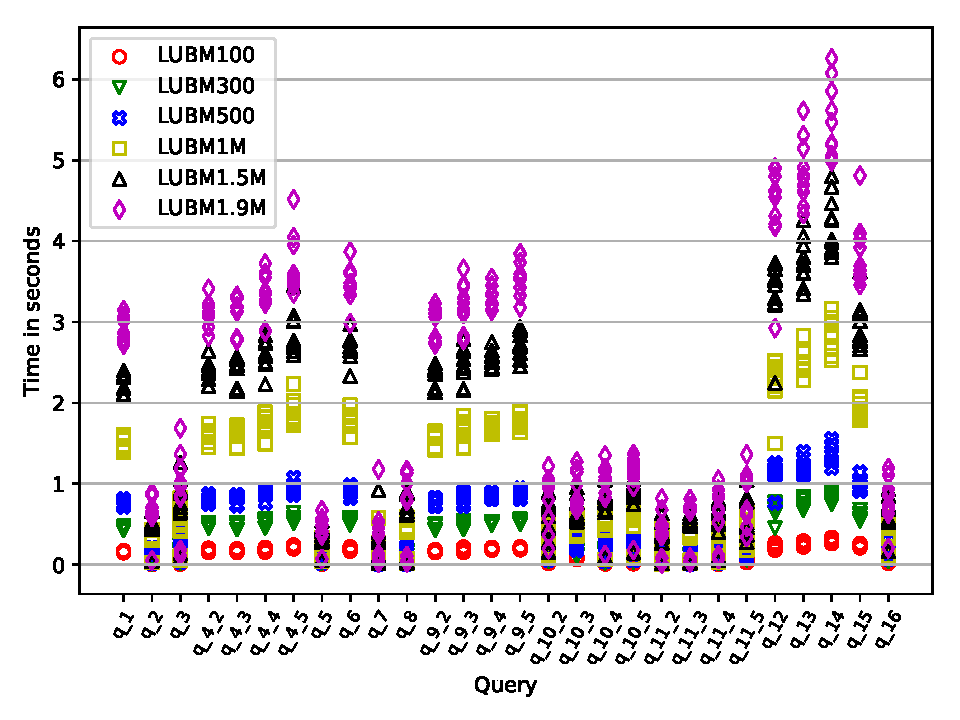
\includegraphics[width=0.48\textwidth]{data/LUBM_all.pdf}
   \caption{Reachability index creation time for LUBM graphs}
   \label{fig:lubm_all_qs}
\end{figure}

Reachability index creation time for each query for for real-world graphs is presented in figure~\ref{fig:other_all_qs}.
We can see that query evaluation time depends on graph inner structure. 
First of all, in some cases handling of small graph requires more time, then handling bigger graph.
For example, $Q_{10}^4$: querying the \textit{geospecies} graph (450k vertices) in some cases requires more time than querying of \textit{mappingbased\_properties} (8.3M vertices) and \textit{taxonomy} (5.7M vertices).
On the other hand, \textit{taxonomy} querying in relatively big number of cases requires significantly more time, than querying of other graphs, while \textit{taxonomy} is not a biggest graph. 
Finally, we can see, that in big number of cases query execution time requires less then 10 seconds, even for big graph, and no queries which require more then 52.17 seconds. 

\begin{figure}
   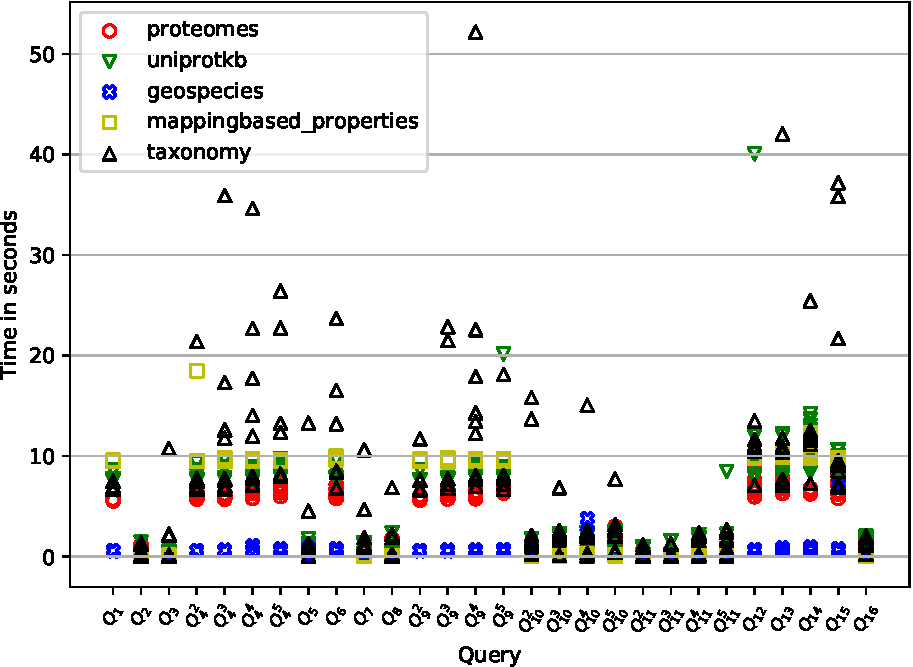
\includegraphics[width=0.48\textwidth]{data/other_all.pdf}
   \caption{Reachability index creation time for real-world RDFs}
   \label{fig:other_all_qs}
\end{figure}

Paths extraction was evaluated on cases with possible long paths.
These cases were selected during reachability index creation by using number of iterations in transitive closure evaluation.
For each selected graph and query we measure paths extraction time for each reachable pair, reachability index creation time is not included because exactly the same index, as calculated at the previous step, is used for paths extraction. 

We evaluate two scenarios.
The first one is a single path extraction.
In this case results are represented as a dependency of extraction time on extracted path length.
We can see linear !!!!

The second scenario is many paths extraction.
Here we limit a number of path to extract by !!! 
In this case results are represented as a dependency of extraction time on number of extracted paths.


\begin{figure}
     \begin{subfigure}[b]{0.24\textwidth}
         \centering
         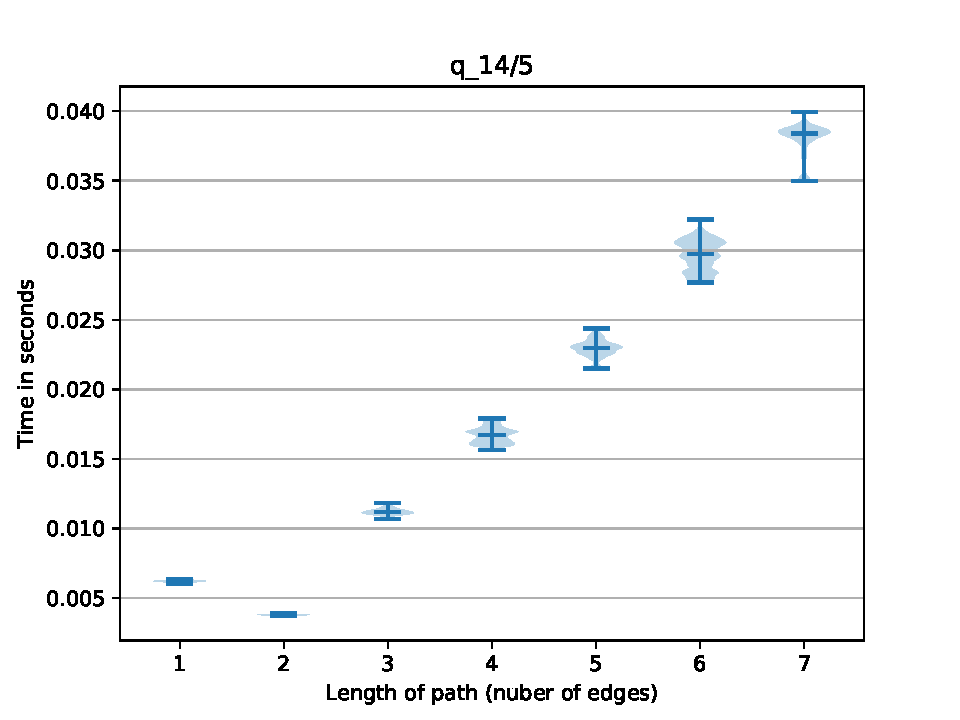
\includegraphics[width=\textwidth]{data/res_graphics/q_14_5.pdf}
         \caption{$y=x$}
         \label{fig:y equals x}
     \end{subfigure}
     ~\begin{subfigure}[b]{0.24\textwidth}
         \centering
         %\includegraphics[width=\textwidth]{data/res_graphics/q9_2_8.pdf}
         \caption{$y=x$}
         \label{fig:y equals x}
     \end{subfigure}\\
     \begin{subfigure}[b]{0.24\textwidth}
         \centering
         %\includegraphics[width=\textwidth]{data/res_graphics/q_14_8.pdf}
         \caption{$y=x$}
         \label{fig:y equals x}
     \end{subfigure}
     ~\begin{subfigure}[b]{0.24\textwidth}
         \centering
         %\includegraphics[width=\textwidth]{data/res_graphics/q4_2_8.pdf}
         \caption{$y=x$}
         \label{fig:y equals x}
     \end{subfigure}
   %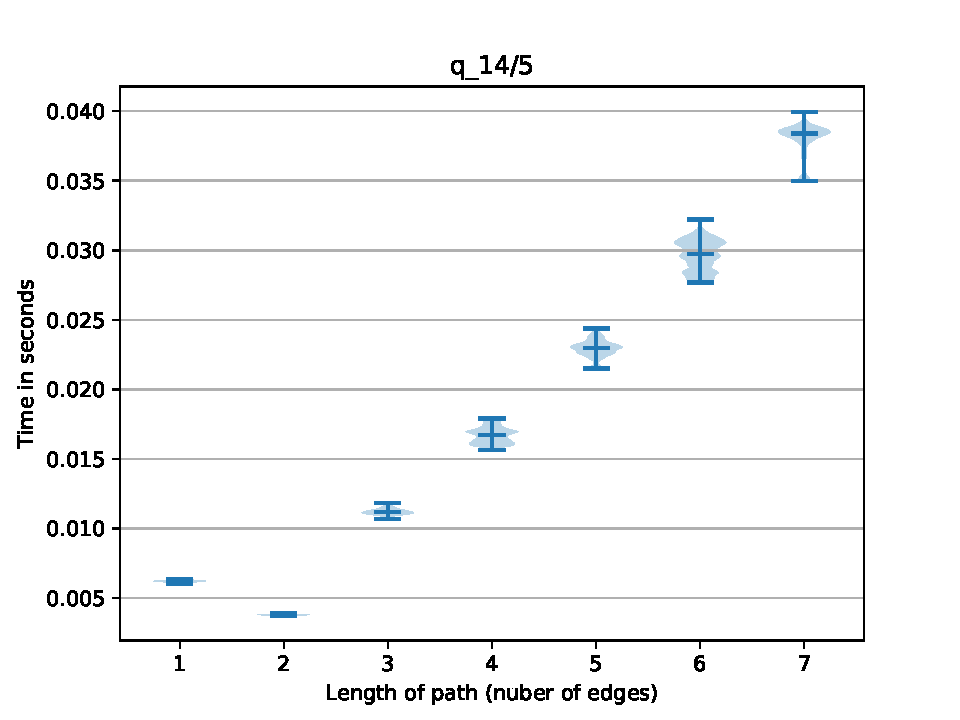
\includegraphics[width=0.48\textwidth]{data/res_graphics/q_14_5.pdf}
   \caption{Single path extraction}
\end{figure}

\subsubsection{Conclusion}

We can conclude that proposed algorithm is applicable for real-world data processing: the algorithm allows one both to solve reachability problem and to extract paths of interest in reasonable time even using na{\"i}ve implementation.  

\subsection{CFPQ Evaluation}

Comparison with matrix-based algorithm.

\subsubsection{Dataset}

Dataset for evaluation. 
It should be CFPQ\_Data\footnote{CFPQ\_Data is a dataset for CFPQ evaluation which contains both synthetic and real-world data and queries \url{https://github.com/JetBrains-Research/CFPQ\_Data}. Access date: 07.07.2020.}

\begin{table}
{
\rowcolors{2}{black!2}{black!10}
\begin{tabular}{|l|c|c|}
\hline
Graph & \#V & \#E \\
\hline
\hline 
eclass\_514en  & 120 926 & 484 646 \\
enzyme  & 358 434 & 144 9711 \\
geospecies  & 596 760 & 2 416 513 \\
go   & 1 188 340 & 4 820 728 \\
go-hierarchy & 1 780 956 & 7 228 358 \\
taxonomy & 2 308 385 & 9 369 511 \\
\hline
Aliases 1 & 6 442 630 & 24 465 430 \\
Aliases 2 & 4 834 262 & 12 366 973 \\
.... & 5 728 398 & 14 922 125 \\
\hline
\end{tabular}
}
\caption{Graphs for CFPQ evaluation}
\label{tbl:graphs_for_cfpq}
\end{table}



Same-generation queries, memory aliases.

\subsubsection{Results}

Results of evaluation.

Index creation.

{\setlength{\tabcolsep}{0.4em}
	\begin{table}
		\caption{RDFs query $G_1$ and $G_2$ (time is measured in seconds and memory is measured in megabytes)}
		\label{tbl:tableRDFQ1_appendix}
		\rowcolors{4}{black!2}{black!10}
		\small
		\begin{tabular}{| l | c | c | c | c |}
			\hline
			
			\multirow{2}{*}{Name}  & \multicolumn{2}{c|}{$G_1$} & \multicolumn{2}{c|}{$G_2$} \\
			\cline{2-5}
			                       & Tensors & RG\_CPU\textsubscript{path} & Tensors & RG\_CPU\textsubscript{path}	 \\
			\hline
			\hline
			eclass\_514en   & 0.254   & 0.195   & 0.227 & ...\\
			enzyme          & 0.035   & 0.029   & 0.036 & ...\\
			geospecies      & 0.091   & ...     & 0.001 & ...\\
			go-hierarchy    & 0.186   & 0.976   & 0.293 & ...\\
			go              & 1.676   & 1.286   & 1.368 & ...\\
			pathways        & 0.015   & 0.021   & 0.009 & ...\\
			taxonomy        & 5.366   & .....   & 3.282 & ...\\
			\hline
		\end{tabular}
	\end{table}
}


Paths extraction.

\subsubsection{Conclusion}

\section{CFPQ algortihms comparison}

Comparison of properties and abilities of CFPQ algorithms.
\begin{itemize}
\item Query format: grammar in specific form, combinators, etc
\item Supported query semantics
\item Supported query types (single source, all pairs, etc)
\item Parallelization
\item ...
\end{itemize}

\section{Conclusion and future work}
In this paper, we shown how the context-free path query evaluation w.r.t. the relational and the single-path query semantics can be reduced to the calculation of matrix transitive closure. Also, we provided a formal proof of the correctness of the proposed reduction. In addition, we introduced an algorithm for computing this transitive closure, which allows us to efficiently apply GPGPU computing techniques. Finally, we shown the practical applicability of the proposed algorithm by running different implementations of our algorithm on real-world data.

We can identify several open problems for further research. In this paper we have considered only two semantics of context-free path querying but there are other important semantics, such as all-path query semantics~\cite{hellingsPathQuerying} which requires to present all paths for all triples $(A,m,n)$. Context-free path querying implemented with algorithm~\cite{GLL} can answer the queries in all-path query semantics by constructing a parse forest. It is possible to construct a parse forest for a linear input by matrix multiplication~\cite{okhotin_cyk}. Whether it is possible to generalize this approach for a graph input is an open question.

In our algorithm, we calculate the matrix transitive closure naively, but there are algorithms for the transitive closure calculation, which are asymptotically more efficient. Therefore, the question is whether it is possible to apply these algorithms for the matrix transitive closure calculation to the problem of context-free path querying.

Also, there are Boolean grammars~\cite{okhotinBoolean}, which have more expressive power than context-free grammars. Boolean path querying is an undecidable problem~\cite{hellingsRelational} but our algorithm can be trivially generalized to work on boolean grammars because parsing with boolean grammars can be expressed by matrix multiplication~\cite{okhotin_cyk}. It is not clear what a result of our algorithm applied to Boolean grammars would look like. Our hypothesis is that it would produce the upper approximation of a solution.

From a practical point of view, matrix multiplication in the main loop of the proposed algorithm may be performed on different GPGPU independently. It can help to utilize the power of multi-GPU systems and increase the performance of context-free path querying.

There is an algorithm~\cite{apspGPU} for transitive closure calculation on directed graphs which generalized to handle graph sizes inherently larger then the DRAM memory available on the GPU. Therefore, the question is whether it is possible to apply this approach to the matrix transitive closure calculation in the problem of context-free path querying.      % Заключение
\clearpage
\phantomsection
\addcontentsline{toc}{chapter}{\bibname}	% Добавляем список литературы в оглавление
\bibliography{biblio}						% Подключаем BibTeX-базы      % Список литературы
\clearpage
\phantomsection
\addcontentsline{toc}{chapter}{\listfigurename}
\listoffigures									% Список изображений
\newpage

%%% Список таблиц %%%
% (ГОСТ Р 7.0.11-2011, 5.3.10)
\clearpage
\phantomsection
\addcontentsline{toc}{chapter}{\listtablename}
\listoftables									% Список таблиц
\newpage           % Списки таблиц и изображений (иллюстративный материал)
%\section{Dataset description}\label{section:dataset}

In our evaluation we use dataset which contains the following parts.
{\setlength{\tabcolsep}{0.4em}
	\begin{table}[h]
		\caption{RDFs properties}
		\label{tbl:propRDF}
		\rowcolors{2}{}{lightgray}
		\begin{tabular}{| l | c | c | c | c |}
			\hline
			Name                  & \#V    & \#E     & \#type &\#subClassOf \\
			\hline
			\hline
			atom-primitive				& 291		& 685		& 138	& 122	\\
			univ-bench					& 179		& 413		& 84		& 36		\\
			travel						& 131		& 397		& 90		& 30		\\
			skos							& 144		& 323		& 70		& 1		\\
			people\_pets					& 337		& 834		& 161	& 33		\\
			generations					& 129		& 351		& 78		& 0		\\
			foaf							& 256		& 815		& 174	& 10		\\
			biomed-mesure-prim   	    & 341		& 711		& 130	& 122	\\
			funding						& 778		& 1480		& 304	& 90               \\
			pizza						& 671		& 2604		& 365	& 259              \\
			wine							& 733		& 2450		& 485	& 126              \\
			core							& 1323		& 8684		& 1412	& 178              \\
			pathways						& 6238		& 37196		& 3118 	& 3117             \\
			go-hierarchy					& 45007		& 1960436	& 0		& 490109           \\
			enzyme						& 48815		& 219390		& 14989	& 8163             \\
			eclass\_514en				& 239111		& 1047454	& 72517	& 90962            \\
			go							& 272770		& 1068622	& 58483	& 90512            \\
			\hline
		\end{tabular}
	\end{table}
}

{\setlength{\tabcolsep}{0.4em}
\begin{table*}[h]
\caption{RDFs query $G_2$ (time is measured in seconds and memory is measured in megabytes)}
\label{tbl:tableRDFQ2}
\rowcolors{3}{}{lightgray}
\begin{tabular}{| l | r  r | r  r | r  r | r  r | r  r |}
    \hline

    \multirow{3}{*}{Name}   &   \multicolumn{6}{|c|}{Relational semantics index}	&	\multicolumn{4}{|c|}{Single path semantics index} \\
    \cline{2-11}
    &	\multicolumn{2}{|c|}{RG\_CPU\textsubscript{rel}}	&	\multicolumn{2}{|c|}{RG\_CUSP\textsubscript{rel}}	&	\multicolumn{2}{|c|}{RG\_SPARSE\textsubscript{rel}} &	\multicolumn{2}{|c|}{RG\_CPU\textsubscript{path}}	&	\multicolumn{2}{|c|}{RG\_SPARSE\textsubscript{path}}	 \\
    \cline{2-11}
    &   Time & Mem &  Time     & Mem & Time     & Mem  &  Time     & Mem & Time     & Mem \\
    \hline
    \hline
    atom-primitive          & 0.001 & 0.3  & 0.001 & 0.1 & 0.002 & 0.1   & 0.001 & 0.3  & 0.002 & 0.1   \\
biomedical-mesure-primitive & 0.002 & 0.1  & 0.014 & 2.0   & 0.009 & 0.1   & 0.006 & 0.1  & 0.012 & 0.1   \\
core                        & 0.001 & 0.3  & 0.006 & 0.1 & 0.004 & 0.1   & 0.003 & 0.3  & 0.005 & 0.1   \\
eclass\_514en               & 0.035 & 6.5  & 0.020 & 16.0  & 0.100   & 12.0    & 0.123 & 17.7 & 0.127 & 18.0    \\
enzyme                      & 0.006 & 3.9  & 0.006 & 0.6 & 0.010  & 0.1   & 0.012 & 5.3  & 0.008 & 0.4   \\
foaf                        & 0.001 & 0.1  & 0.004 & 0.1 & 0.002 & 0.1   & 0.001 & 0.1  & 0.003 & 0.1   \\
funding                     & 0.002 & 0.1  & 0.015 & 0.4 & 0.007 & 0.1   & 0.009 & 0.1  & 0.008 & 0.1   \\
generations                 & 0.001 & 0.1  & 0.001 & 0.1 & 0.001 & 0.1   & 0.001 & 0.1  & 0.001 & 0.1   \\
go-hierarchy                & 0.095 & 17.8 & 0.253 & 528.0 & 0.175 & 130.4 & 0.884 & 88.8 & 0.306 & 138.8 \\
go                          & 0.306 & 25.8 & 0.240 & 84.0  & 0.181 & 25.4  & 0.918 & 78.1 & 0.219 & 34.2  \\
pathways                    & 0.005 & 0.2  & 0.005 & 0.4 & 0.004 & 0.1   & 0.017 & 0.5  & 0.003 & 0.1   \\
people\_pets                & 0.001 & 0.1  & 0.007 & 0.1 & 0.004 & 0.1   & 0.001 & 0.1  & 0.005 & 0.1   \\
pizza                       & 0.002 & 0.3  & 0.012 & 0.2 & 0.008 & 0.1   & 0.010  & 0.3  & 0.009 & 0.1   \\
skos                        & 0.001 & 0.1  & 0.001 & 0.1 & 0.001 & 0.1   & 0.001 & 0.1  & 0.002 & 0.1   \\
travel                      & 0.001 & 0.1  & 0.007 & 0.1 & 0.005 & 0.1   & 0.001 & 0.1  & 0.005 & 0.1   \\
univ-bench                  & 0.001 & 0.1  & 0.007 & 0.1 & 0.005 & 0.1   & 0.001 & 0.1  & 0.005 & 0.1   \\
wine                        & 0.001 & 0.3  & 0.006 & 0.1 & 0.004 & 0.1   & 0.002 & 0.3  & 0.004 & 0.1  \\
    \hline
  \end{tabular}
\end{table*}
}

\begin{itemize}
\item The real-world data RDFs provided in CFPQ\_Data dataset\footnote{CFPQ\_Data dataset GitHub repository: \url{https://github.com/JetBrains-Research/CFPQ_Data}. Access date: 12.11.2019.} from~\cite{Mishin:2019:ECP:3327964.3328503}.
\item Geospecies (RDF which contains information about biological hierrarchy\footnote{The Geospecies RDF: \url{https://old.datahub.io/dataset/geospecies}. Access date: 12.11.2019.} and same-generation query over \textit{broaderTransitive} relation) is provided in~\cite{Kuijpers:2019:ESC:3335783.3335791} and integrated in our evaluation with CFPQ\_Data.
\item It was shown in~\cite{Mishin:2019:ECP:3327964.3328503} that matrix-based algorithm is performant enough to handle bigger RDFs than those used in the initial datasets, such as~\cite{RDF}.
So, we add several big RDFs to CFPQ\_Data and use them in our evaluation.
New RDFs: \textit{go-hierarchy, go, enzime, core, pathways} are from UniProt database\footnote{Protein sequences data base: \url{https://www.uniprot.org/}. RDFs with data are avalable here: \url{ftp://ftp.uniprot.org/pub/databases/uniprot/current_release/rdf}. Access date: 12.11.2019}, and \textit{eclass-514en} is from eClassOWL project\footnote{eClassOWL project: \url{http://www.heppnetz.de/projects/eclassowl/}. eclass-514en file is available here: \url{http://www.ebusiness-unibw.org/ontologies/eclass/5.1.4/eclass_514en.owl}. Access date: 12.11.2019.}.
\end{itemize}

The properties of the RDFs from the dataset are given in table \ref{tbl:propRDF}. 
Geospecies RDF contains 450609 vertices, 2311461 edges, and 20867 edges labeled by \textit{broaderTransitive}.
Note that while the number of edges labeled by \textit{broaderTransitive} is equal to provided in~\cite{Kuijpers:2019:ESC:3335783.3335791}, the total number of vertices and edges is bigger. It is because we naively convert each triple from RDF to edge in the graph, while J. Kuijpers et al. use special \textit{neosemantics}\footnote{Neosemantix is an RDF processing plugin for Neo4j. Web page: \url{https://neo4j.com/labs/nsmtx-rdf/}. Access date: 30.03.2020.} plugin which can, for example, handling multivalued properties accurately.  

The variants of the \textit{same-generation query}~\cite{FndDB} are used in almost all cases because it is an important example of real-world queries that are context-free but not regular.
So, variations of the same generation query are used in our evaluation.
All queries are added to the CFPQ\_Data dataset.

We use two queries over \textit{subClassOf} and \textit{type} relations.
The first query is the grammar $G_1$:
\[
 \begin{array}{lcl}
   s  \rightarrow \textit{subClassOf}^{\ -1} \ s \ \textit{subClassOf}   & \quad & s  \rightarrow \textit{type}^{\ -1} \ s \ \textit{type}     \\
   s  \rightarrow \textit{subClassOf}^{\ -1} \ \textit{subClassOf}       & \quad & s  \rightarrow  \textit{type}^{\ -1}  \ \textit{type}

 \end{array}
 \]
The second one is the grammar $G_2$: \[s \rightarrow \textit{subClassOf}^{\ -1} \ s \ \textit{subClassOf} \mid \textit{subClassOf}\]

For geospecies we use same-generation query \textit{geo} from the original paper~\cite{Kuijpers:2019:ESC:3335783.3335791}: \[s \rightarrow \textit{broaderTransitive} \ s \ \textit{broaderTransitive}^{\ -1} \]
\[s \rightarrow \textit{broaderTransitive}  \ \textit{broaderTransitive}^{\ -1} \]


\section{Evaluation Details}

Results for RDFs querying with $G_2$ grammar are presented in table~\ref{tbl:tableRDFQ2}.
We can see, that for small graphs time for both relational and single-path querying are similar for CPU and GPGPU versions, but for bigger graphs (\textit{go} and \textit{go-hierarchy}, for example) GPUPU version is more performant than CPU one.

\balance

        % Приложения

\end{document}
